%------------------------------------------------------------------------------
%                      Template Naskah Skripsi
%               	Berdasarkan format JTETI FT UGM
% 						         (c) @gunturdputra 2014
%-------------------------------------------------------------------------------

%Template pembuatan naskah skripsi.
\documentclass{jtetiskripsi}

%Untuk prefiks pada daftar gambar dan tabel
\usepackage[titles]{tocloft}
\renewcommand\cftfigpresnum{Gambar\  }
\renewcommand\cfttabpresnum{Tabel\   }

%Untuk hyperlink dan table of content
\usepackage[hidelinks]{hyperref}
\newlength{\mylenf}
\settowidth{\mylenf}{\cftfigpresnum}
\setlength{\cftfignumwidth}{\dimexpr\mylenf+2em}
\setlength{\cfttabnumwidth}{\dimexpr\mylenf+2em}

%Untuk Bold Face pada Keterangan Gambar
\usepackage[labelfont=bf]{caption}

%Untuk caption dan subcaption
\usepackage{caption}
\usepackage{subcaption}

%pdf
\usepackage{pdfpages}

%table
\usepackage{graphics}

\usepackage{wrapfig}

%bibliography
\usepackage{natbib}

%equation
\usepackage{amsmath}

% long table
\usepackage{longtable}

%algoritma
\usepackage{algorithm}
\usepackage{algpseudocode}

%listing
\usepackage{listings}

\definecolor{codegreen}{rgb}{0,0.6,0}
\definecolor{codegray}{rgb}{0.5,0.5,0.5}
\definecolor{codepurple}{rgb}{0.58,0,0.82}
\definecolor{backcolour}{rgb}{0.95,0.95,0.92}

\lstdefinestyle{unjstyle} {
  frame=top, frame=bottom,
  breakatwhitespace=false,         
  breaklines=true,                 
  captionpos=t,
  % backgroundcolor=\color{backcolour},   
  commentstyle=\color{codegreen},
  keywordstyle=\color{magenta},
  numberstyle=\tiny\color{codegray},
  stringstyle=\color{codepurple}
}
\lstset{style=unjstyle}

%-----------------------------------------------------------------
%Disini awal masukan untuk data proposal skripsi
%-----------------------------------------------------------------
\titleind{Perancangan Improvisasi Arsitektur \emph{Web Crawler} Berbasis \emph{Multi-Threading} dan \emph{Multi-Processing} Dengan Menggunakan Bahasa Pemrograman \emph{Rust}}

\fullname{Muhammad Daffa Haryadi Putra}

\idnum{1313619034}

%\approvaldate{12 Februari 2019}
\approvaldate{12 Februari 2019}

\degree{Sarjana Ilmu Komputer}

\yearsubmit{2024}

\program{Ilmu Komputer}

\dept{Ilmu Komputer}

\firstsupervisor{Muhammad Eka Suryana, M. Kom.}
\firstnip{198512232012121002}

\secondsupervisor{Med Irzal, M. Kom.}
\secondnip{197706152003121001}

%-----------------------------------------------------------------
%Disini akhir masukan untuk data proposal skripsi
%-----------------------------------------------------------------

\tolerance=1
\emergencystretch=\maxdimen
\hyphenpenalty=10000
\hbadness=10000

\begin{document}

\cover

% 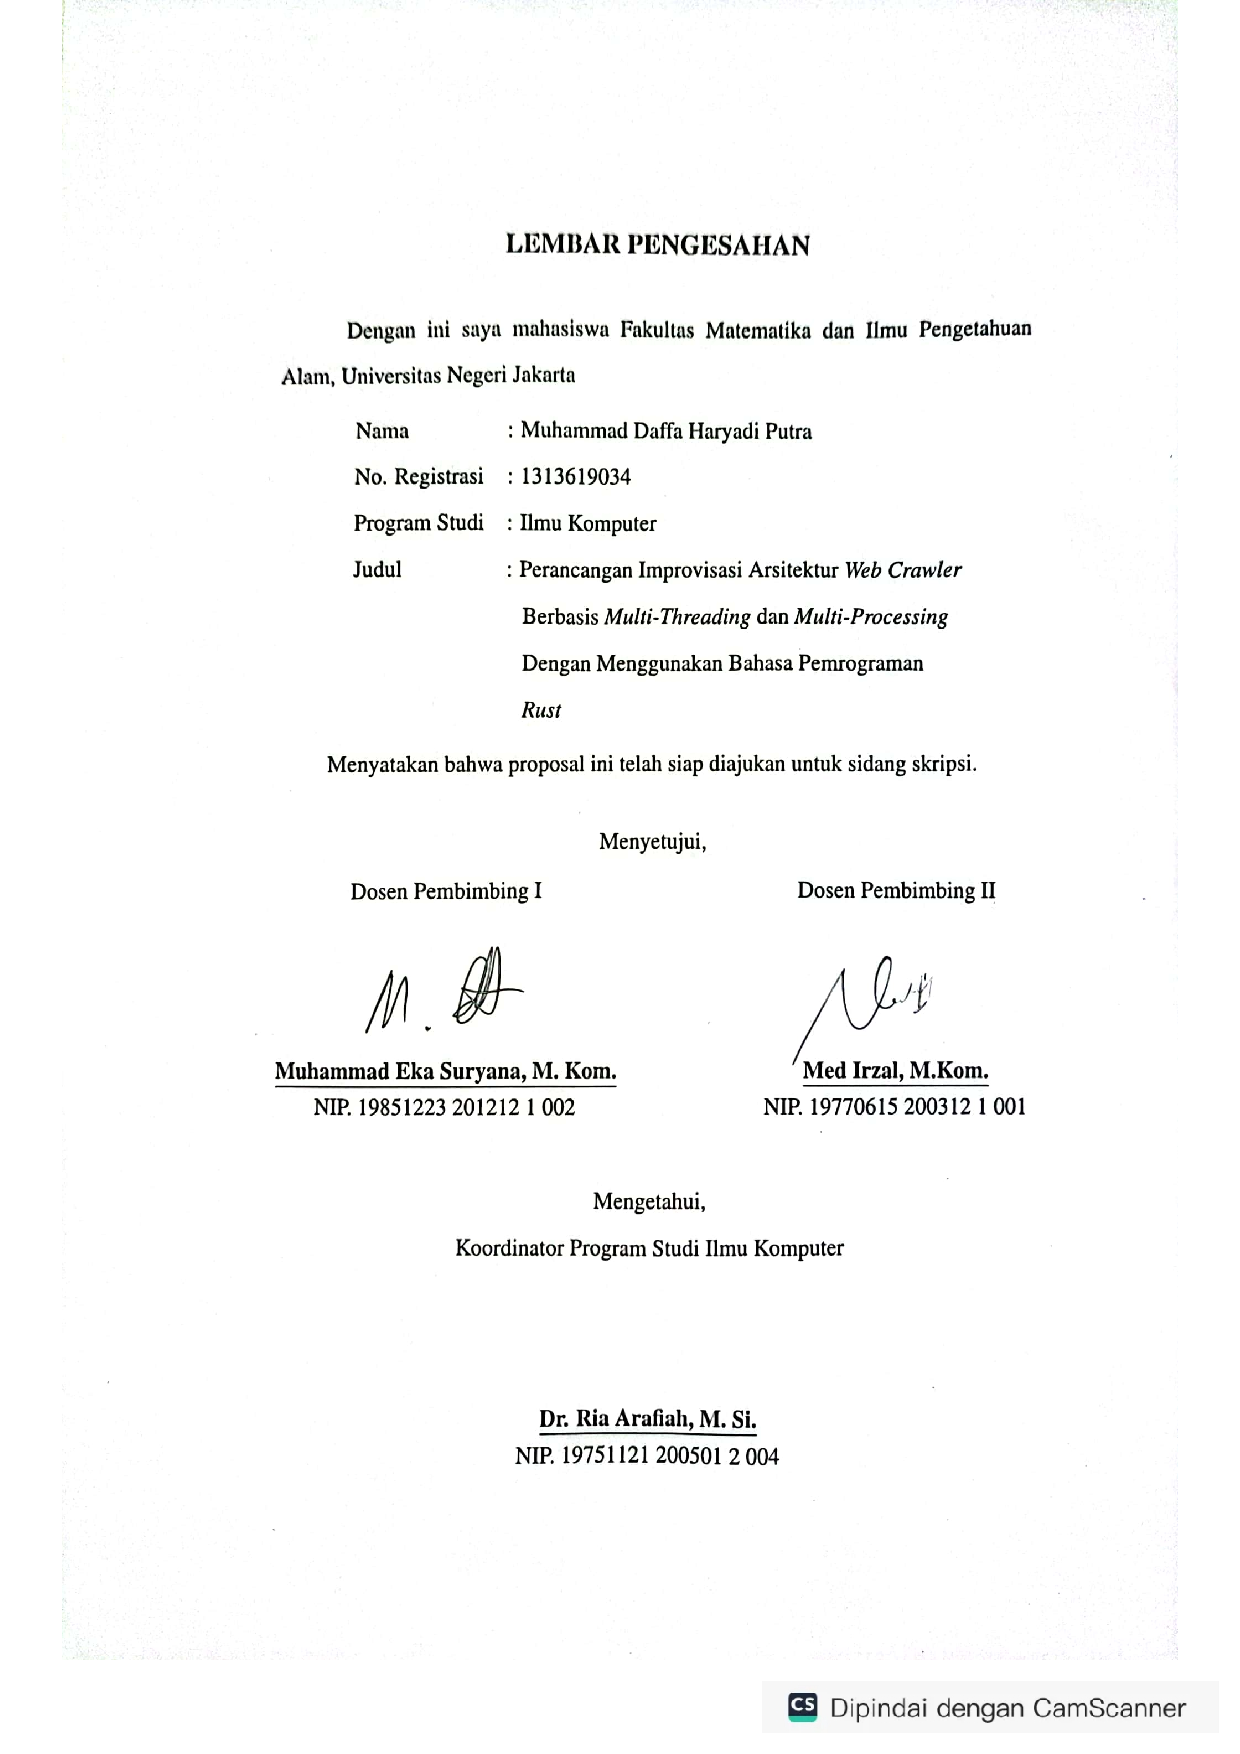
\includepdf[pages=-]{pdf/lembar-pengesahan.pdf}
% \chapter*{\centering{\large{\thesisapprovalname}}}
\thispagestyle{empty} {\bf }
\vspace{-0.5cm}
\begin{center}
	\textbf{Desain Perancangan \emph{Crawler} Sebagai Pendukung pada \emph{Search Engine}}
\end{center}

\vspace{1mm}
\vskip 1.5mm \noindent
\begin{tabular}{ll}
	\hskip-2mm Nama & : Muhammad Fathan Qoriiba \\
	\hskip-2mm No. Registrasi & : 3145161299 \\
\end{tabular}


\vskip2mm

\noindent \begin{flushleft}
	\begin{tabular}{llcc}
		
		& \hskip15mm \textbf{Nama} & \textbf{Tanda Tangan} & \textbf{Tanggal} \\
		
		\hskip-1cm \textbf{Penanggung Jawab} &  &  &  \\
		\hskip-1cm Dekan & : Prof. Dr. Muktiningsih N, M.Si. & ............... & ............. \\
		& \hskip3mm NIP. 19640511 198903 2 001 &  &  \\
		\hskip-1cm \textbf{Wakil Penanggung Jawab} &  &  &  \\
		\hskip-1cm Wakil Dekan Bidang Akademik & : Dr. Esmar Budi, S.Si., MT. & ............... & ............. \\
		& \hskip3mm NIP. 19720728 199903 1 002 &  &  \\
		\hskip-1cm Ketua & : Drs. Mulyono, M.Kom. & ............... & ............. \\
		& \hskip3mm NIP. 19660517 199403 1 003 &  &  \\
		\hskip-1cm Sekretaris & : Ari Hendarno, S.Pd, M.Kom & ............... & ............. \\
		& \hskip3mm NIDK. 8857650017 &   &  \\	
		\hskip-1cm Penguji Ahli & : Ria Arafiyah, M.Si. & ............... & ............. \\
		& \hskip3mm NIP. 19751121 200501 2 004 &  &  \\
		\hskip-1cm Pembimbing I & : Med Irzal, M.Kom. & ............... & ............. \\
		& \hskip3mm NIP. 19770615 200312 1 001 &  &  \\		
		\hskip-1cm Pembimbing II & : Muhammad Eka Suryana, M.Kom. & ............... & ............. \\
		& \hskip3mm NIP. 19851223 201212 1 002 &  &  \\
	\end{tabular}
\end{flushleft}

\vskip1mm

\noindent \textbf{Dinyatakan lulus ujian skripsi tanggal: 04 Agustus 2021}


% \chapter*{\centering{\large{LEMBAR PERNYATAAN}}}

Saya menyatakan dengan sesungguhnya bahwa skripsi dengan judul 	\textbf{Desain Perancangan \emph{Crawler} Sebagai Pendukung pada \emph{Search Engine}} yang disusun sebagai syarat untuk memperoleh gelar Sarjana komputer dari Program Studi Ilmu Komputer Universitas Negeri Jakarta adalah karya ilmiah saya dengan arahan dari dosen pembimbing.

Sumber informasi yang diperoleh dari penulis lain yang
telah dipublikasikan yang disebutkan dalam teks skripsi ini, telah dicantumkan dalam Daftar Pustaka sesuai dengan norma, kaidah dan etika penulisan ilmiah.

Jika dikemudian hari ditemukan sebagian besar skripsi ini bukan hasil karya saya sendiri dalam bagian-bagian tertentu, saya bersedia menerima sanksi pencabutan gelar akademik yang saya sanding dan sanksi-sanksi lainnya sesuai dengan peraturan perundang-undangan yang berlaku.

\vspace{.5cm}

\begin{tabular}{p{7.5cm}c}
	&Jakarta, 26 Julii 2021\\
	&\\
	&\\
	&\\
	&Muhammad Fathan Qoriiba
\end{tabular}

\chapter*{\centering{\large{LEMBAR PERNYATAAN}}}
\onehalfspacing{}

Saya menyatkan dengan sesungguhnya bahwa skripsi dengan judul
\textbf{"Perancangan Improvisasi Arsitektur Web Crawler Berbasis Multi-Threading dan Multi-Processing Dengan Menggunakan Bahasa Pemrograman Rust"} yang disusun sebagai syarat untuk memperoleh gelar Sarjana Komputer
dari Program Studi Ilmu Komputer Universitas Negeri Jakarta adalah karya ilmiah
saya dengan arahan dari dosen pembimbing.

Sumber informasi yang diperoleh dari peneliti lain yang telah dipublikasikan 
yang disebutkan dalam teks Skripsi ini, telah dicantumkan dalam Daftar Pustaka 
sesuai dengan norma, kaidan dan etika penulisan ilmiah.

Jika dikemudian hari ditemukan sebagian besar skripsi ini bukan hasil karya saya 
sendiri dalam bagian-bagian tertentu, saya bersedia menerima sanksi pencabutan 
gelar akademik yang saya sanding dan sanksi-sanksi lainnya sesuai dengan 
peraturan perundang-undangan yang berlaku.

\vspace{4cm}

\begin{tabular}{p{7.5cm}c}
	&Jakarta, 26 Juli 2024\\
	&\\
	&\\
	&\\
	&Muhammad Daffa Haryadi Putra
\end{tabular}


%-----------------------------------------------------------------
%Disini awal masukan Acknowledment
%-----------------------------------------------------------------
\acknowledgment
\begin{flushright}
	\emph{Untuk Mamah dan Ayah.}
\end{flushright}

\chapter*{\centering{\large{KATA PENGANTAR}}}
\onehalfspacing{}
Puji syukur penulis panjatkan ke hadirat Allah SWT, karena dengan rahmat dan
karunia-Nya, penulis dapat menyelesaikan proposal skripsi yang berjudul
\textit{Perancangan Improvisasi Arsitektur Web Crawler Berbasis Multi-Threading dan Multi-Processing Dengan Menggunakan Bahasa Pemrograman Rust}.

Keberhasilan dalam penyusunan proposal skripsi ini tidak lepas dari bantuan
berbagai pihak yang mana dengan tulus dan ikhlas memberikan masukan guna
sempurnanya proposal skripsi ini. Oleh karena itu dalam kesempatan ini, dengan
kerendahan hati penulis mengucapkan banyak terima kasih kepada:

\begin{enumerate}

	\item{Yth. Para petinggi di lingkungan FMIPA Universitas Negeri Jakarta.}
	\item{Yth. Ibu Dr. Ria Arafiyah, M.Si selaku Koordinator Program Studi Ilmu
		Komputer.}
	\item{Yth. Bapak Muhammad Eka Suryana, M.Kom selaku Dosen Pembimbing I yang
		telah membimbing, mengarahkan, serta memberikan saran dan koreksi terhadap
		proposal skripsi ini.}
	\item{Yth. Bapak Med Irzal, M.Kom selaku Dosen Pembimbing II yang telah
		membimbing, mengarahkan, serta memberikan saran dan koreksi terhadap
		proposal skripsi ini.}
	\item{Kedua orang tua dan adik penulis yang telah mendukung dan memberikan 
		semangat serta doa untuk penulis.}
  \item{Teman-Teman dari Warung Tegang dengan segala keunikan dan keanehannya yang 
    selalu memberikan semangat dan motivasi bagi penulis untuk menyelesaikan 
    skripsi ini}
  \item{Teman-Teman dari Rabbit Hole Club dengan segala keunikannya yang selalu
    memberikan motivasi bagi penulis dalam menyelesaikan skripsi ini}
  \item{Teman-Teman dari grup telegram Teknologi Umum terkhusus Mustafa yang telah 
    memberikan konsultasi dalam pengerjaan skripsi ini}
	\item{Nakiri Ayame, Vestia Zeta, dan Ayunda Risu dari Hololive yang telah 
    menemani malam-malam penulis dalam mengerjakan skripsi}
	\item{Teman-teman Program Studi Ilmu Komputer 2019 yang telah memberikan 
		dukungan dan memiliki andil dalam penulisan proposal skripsi ini.}
	\item{Juned, Saipul, dan kucing-kucing penulis yang telah memberikan motivasi
    mental kepada penulis selama pengerjaan skripsi}
	
\end{enumerate}

Penulis menyadari bahwa penyusunan proposal skripsi ini masih jauh dari sempurna
karena keterbatasan ilmu dan pengalaman yang dimiliki. Oleh karenanya, kritik
dan saran yang bersifat membangun akan penulis terima dengan senang hati. Akhir
kata, penulis berharap tugas akhir ini bisa bermanfaat bagi semua pihak
khususnya penulis sendiri. Semoga Allah SWT senantiasa membalas kebaikan semua
pihak yang telah membantu penulis dalam menyelesaikan proposal skripsi ini.

\vspace{4cm}

\begin{tabular}{p{7.5cm}c}
	&Jakarta, 26 Juli 2024\\
	&\\
	&\\
	&\\
	&Muhammad Daffa Haryadi Putra
\end{tabular}

\addcontentsline{toc}{chapter}{KATA PENGANTAR}

%-----------------------------------------------------------------
%Disini awal masukan Intisari
%-----------------------------------------------------------------
\begin{abstractind}
\textbf{MUHAMMAD DAFFA HARYADI PUTRA}. Perancangan Improvisasi Arsitektur \emph{Web Crawler} Berbasis \emph{Multi-Threading} dan \emph{Multi-Processing} Dengan Menggunakan Bahasa Pemrograman \emph{Rust}. Skripsi. Fakultas Matematika dan Ilmu Pengetahuan Alam, Universitas Negeri Jakarta. 2024. Di bawah bimbingan Muhammad Eka Suryana, M. Kom dan Med Irzal, M. Kom.
\vskip1cm
	
  Mesin pencari atau \emph{search engine} merupkan \emph{software} yang digunakan untuk melakukan pencarian terhadap informasi tertentu. Untuk menjalankan proses pencarian diperlukan jumlah data yang banyak yang terkumpul dan dapat diakses dengan mudah, proses pengumpulan data ini lah yang disebut \emph{crawling}. Penelitian ini mencoba untuk memperbaiki kekurangan-kekurangan dari \emph{crawler} versi lazuardy dengan penekanan dalam efisiensi peforma dan penggunaan \emph{computing resource}. Penelitian ini menggunakan metode \emph{multi-threading} dan \emph{multi-processing} untuk membagi beban tugas kerja dari \emph{crawler} menjadi dua modul yaitu, \emph{scouter} dan \emph{parser}, selain itu algoritma \emph{breadth-first search} yang digunakan dalam \emph{crawler} dimodifikasi untuk membatasi halaman web apa yang dapat di jelajahi oleh \emph{crawler}. Hasil akhir dari penelitian ini menunjukkan bahwa terdapat improvisasi dengan metode baru ini sebesar 17x dibandingkan dengan \emph{crawler} orisinil, dengan catatan penyeratan halaman terunduh antar \emph{domain} belum berhasil.
	
	\bigskip
	\noindent
  \textbf{Kata kunci :} \textit{Crawler}, \textit{search engine}, \textit{Rust Programming Language}, \textit{multi-threading}, \textit{multi-processing}
\end{abstractind}
%
\begin{abstracteng}

  \textbf {MUHAMMAD DAFFA HARYADI PUTRA}. \emph{Design Improvement on Crawler Architecture Based on Multi-threading and Multi-processing using Rust Programming Language. Mini Thesis. Faculty of Mathematics and Natural Sciences, State University of Jakarta. 2024. Under the guidence of} Muhammad Eka Suryana, M. Kom \emph{and} Med Irzal, M. Kom.
\vskip1cm

  Search engine are a software used to do a query for certain information. To run the query process, needed large size of data gathered on one place and could be accessed easily, this process of gathering those data called crawling. This research aims to fix and improve deficiency founded on previous research on crawler and search engine in general by lazuardy khatulistiwa with the emphasis on eficiency and performance of the crawler itself. This research will implemented multi-threading and multi-processing to share the workload of the crawler as two modules, scouter and parser. Besides that, this research also employed a modified breadth-first search algogithm to increase efficiency and limit what kind of page can be crawled. Final result shown that this research successfully improved the performance of the crawler by 17x with some notes that the distribution of each domain downloaded by this crawler hasn't equally distributed yet.

\bigskip
\noindent
\textbf {Keywords:} Crawler, search engine, Rust Programming Language, multi-threading, multi-processing
\end{abstracteng}
%-----------------------------------------------------------------
%Disini akhir masukan Intisari
%-----------------------------------------------------------------
%-----------------------------------------------------------------

%-----------------------------------------------------------------
%Disini akhir masukan untuk muka skripsi
%-----------------------------------------------------------------

\tableofcontents 
\addcontentsline{toc}{chapter}{DAFTAR ISI}
\listoffigures
\addcontentsline{toc}{chapter}{DAFTAR GAMBAR}
\listoftables
\addcontentsline{toc}{chapter}{DAFTAR TABEL}

\begin{counterpage}
\end{counterpage}
%Disini awal masukan untuk Bab
%-----------------------------------------------------------------

%!TEX root = ./template-skripsi.tex
%-------------------------------------------------------------------------------
% 								BAB I
% 							LATAR BELAKANG
%-------------------------------------------------------------------------------

\chapter{PENDAHULUAN}

\section{Latar Belakang Masalah}

% Intro to Search engine architecture and web crawler
\emph{Search engine} merupakan sebuah program yang digunakan untuk menjelajahi dan mencari informasi dari web \citep{seymour2011history}. Terdapat beberapa komponen yang membangun arsitektur \emph{Search engine} seperti \emph{Web crawler}, \emph{Page rank}, dan \emph{indexer} \citep{brin1998anatomy}. Dalam proses pencarian web yang dilakukan \emph{Search engine} tahap pertama yang di lakukan adalah \emph{Web crawler} menjelajahi dan mengekstraksi data-data dari list \emph{url} lalu menyimpan data tersebut dan data lain yang terkait ke dalam database \citep{brin1998anatomy}. Data yang disimpan akan di-index, diberikan skor dan di urutkan melalui algoritma \emph{pagerank} \citep{brin1998anatomy}.

% Analysis for past web crawler, algorithm, architecture, and tech stack
\emph{Web Crawler} merupakan komponen penting dalam pembuatan arsitektur \emph{Search engine} secara keseluruhan. Penelitian sebelumnya yang telah dilakukan oleh \emph{Lazuardy Khatulisitwa} telah berhasil mengimplementasikan \emph{Web crawler} kedalam arsitektur \emph{Search engine} yang berjalan \citep{lazuardithesis}. \emph{Web crawler} tersebut mengimplentasikan algoritma \emph{Breadth First Search} dengan modifikasi algoritma \emph{similiarity based} untuk meningkatkan akurasi dari proses \emph{crawling} dan pengambilan data dari  suatu halaman \citep{lazuardithesis}. Algoritma \emph{Modified Similarity-Based} yang digunakan oleh \emph{Fathan} untuk memperbaiki akurasi dari \emph{Breadth First Search} memanfaatkan konsep penyimpanan \emph{queue} dalam melakukan proses \emph{crawling} \citep{fathanthesis} . Dalam proses tersebut \emph{crawler} akan menyimpan 2 jenis \emph{queue} yaitu, \emph{hot queue} untuk menyimpan \emph{url} yang mengandung kata \emph{anchor} sedangkan \emph{url queue} digunakan untuk menyimpan \emph{url} lain \citep{cho1998efficient}. Proses ini dapat membantu \emph{crawler} untuk mengunjungi dan melakukan \emph{crawling} ke dalam \emph{page} yang terdapat di \emph{hot queue} terlebih dahulu, bila \emph{page} yang berkaitan dengan kata \emph{anchor} di kunjungi terlebih dahulu maka \emph{child page}-nya kemungkinan besar akan memiliki konten yang berkaitan dengan kata \emph{anchor} tersebut \citep{cho1998efficient}. 

Arsitektur dari \emph{crawler} yang di kembangkan oleh Lazuardi, menggunakan \emph{python} sebagai bahasa pemograman dan \emph{library} pendukung yang digunakan adalah \emph{beautifulsoup4} untuk melakukan \emph{parsing} dari halaman \emph{website}, \emph{request} untuk mengirimkan request kepada halaman \emph{website} yang ingin di ambil data-nya, dan \emph{regex} untuk melakukan pencocokan kata - kata yang telah di dapat dengan \emph{keyword} yang sudah di tentukan \citep{lazuardithesis}. Dari hasil penelitian \emph{lazuardi} terdapat beberapa saran peningkatan yang tercatat, dimana salah satunya terkait dengan meningkatkan kinerja dan peforma dari \emph{web crawler} agar memiliki penggunaan \emph{RAM} yang lebih kecil dan mencapai kinerja yang maksimal \citep{lazuardithesis}.

Kinerja atau performa dari \emph{web crawler} dapat dinilai dari waktu yang diperlukan oleh \emph{web crawler} dalam menjalankan fungsi-fungsi nya. Semakin cepat waktu eksekusi dari fungsi dalam \emph{web crawler}, semakin cepat satu halaman di proses dan semakin banyak informasi yang disimpan. Informasi terkait waktu yang dilewati oleh \emph{crawler} per bagian dan bagian apa yang menghambat performa program, dapat dilakukan dengan \emph{profiling}. \emph{Profiling} adalah mekanisme dalam menghitung waktu per-pemanggilan fungsi atau bagian dari kode sehingga dapat ditentukan bagian mana dalam kode yang paling menghambat performa program. \emph{Profiling} yang dilakukan di \emph{crawler} milik lazuardy, menggunakan \emph{line profiler} sebagai alat pembantu. Target dari \emph{profiling} merupakan modul \emph{crawler} dalam file \emph{crawl.py}, fungsi, dan metode-metode lain yang dipanggil oleh modul tersebut. Profiling ini dilakukan selama 6 jam dan menggunakan 4 \emph{threads} dengan taret \emph{url} sejumlah 3.

\begin{table}[H]
  \caption{Hasil \emph{profiling} crawler lazuardy}
  \begin{center}
    \begin{tabular}{ |p{1cm}|p{5cm}|p{4cm}|p{3cm}| } \hline
      \multicolumn{4}{|c|}{Hasil Profiling} \\ \hline
      No.& Nama Operasi& \emph{Library}& Waktu Operasi Rata-Rata (ms) \\ \hline
      1& Pengunduhan halaman \emph{website}& \emph{request}& 1,000 ms \\ \hline
      2& Penyusunan \emph{language tree}& \emph{beautifulsoup4}& 280.5 ms \\ \hline
      3& Pengambilan data dari \emph{queue}& \emph{queue}& 160.1 ms \\ \hline
    \end{tabular}
  \end{center}
\end{table}

Dari hasil \emph{profiling} dapat dilihat bahwa \emph{bottleneck} terbesar adalah proses pemanggilan \emph{request method} terhadap \emph{page}, proses ini memakan waktu rata-rata 1,000 ms atau 1 sekon yaitu sekitar 27 persen dari keseluruhan waktu pemrosesan satu halaman \emph{website}, diikuti oleh proses pembuatan \emph{language tree} yang memakan waktu rata-rata 280.5 ms per pemanggilan, dan pengambilan data \emph{url} dari \emph{queue}. Walaupun arsitektur \emph{search engine} milik lazuardy sudah menerapkan \emph{multi-threading} dalam proses \emph{scraping} per halamannya, antara proses penguduhan halaman dan penyusunan \emph{language tree} masih berada di dalam satu \emph{threads of execution} yang berarti kedua proses itu berjalan secara berurutan, ini mengakibatkan perlambatan yang signifikan dalam proses penjelajahan \emph{crawler} pada satu website dengan domain yang sama. Perbaikan yang dapat dilakukan berdasarkan fakta tersebut adalah dengan menggunakan protokol dan metode pengunduhan halaman \emph{website} yang lebih baik, pemisahan proses pengunduhan dan pembangunan \emph{language tree} sehingga dapat berjalan secara bersamaan, dan menggunakan bahasa pemograman yang memiliki efisiensi peforma yang lebih baik dari arsitekur saat ini.

Salah satu metode untuk mempercepat jalannya \emph{search engine} adalah \emph{Multi-threading} \citep{multithreadedtextsearch}. Metode ini sudah pernah digunakan dalam \emph{search engine} sebelumnya, tetapi \emph{search engine} ini mencari data bukan ke \emph{web} tetapi pada kumpulan data teks atau dapat disebut dengan nama \emph{text search} \citep{multithreadedtextsearch}. Dari hasil penelitian tersebut ditemukan metode \emph{multi-threading} yang digunakan berhasil mencapai improvisasi yang sebelumnya membutuhkan waktu 16 menit dalam menjelajahi seluruh data teks menjadi 4 menit, yang berarti berhasil mencapai improviasi waktu eksekusi program sebesar 4x \citep{multithreadedtextsearch}. Dalam penelitian tersebut metode \emph{multi-threading} digunakan untuk memecah proses pengambilan data dari sumber data dan proses parsing dari data teks yang sudah di ambil \citep{multithreadedtextsearch}.

Dalam konteks \emph{search engine} untuk pencarian web penelitian yang dilakukan oleh \emph{Pramudita, Y.D et all} telah menunjukkan bahwa mekanisme \emph{multi-threading} dapat diimplementasi dengan benar \citep{Pramudita_2020}. Dalam penelitian tersebut tiap-tiap \emph{thread} menjalankan satu \emph{instance} dari \emph{crawler} nya itu sendiri, dan penelitian tersebut berhasil mencapai percepatan waktu \emph{crawling} selama 123 detik \citep{Pramudita_2020}.

Selanjutnya penelitian hanya akan melakukan improvisasi terhadap komponen \emph{web crawler} saja untuk membatasi area penelitian. Penelitian ini akan berusaha untuk meningkatkan performa, yang dimana merupakan jumlah halaman yang terkumpul pada waktu yang sudah definisikan. Berdasarkan hasil penelitian \emph{Pramudita, Y.D et all}, yang dimana menjalankan keseluruhan proses \emph{crawler} dalam satu thread \citep{Pramudita_2020}, maka penelitian ini akan berusaha untuk meningkatkan performa dengan memisahkan proses \emph{parsing} dalam \emph{crawler} dalam proses yang berbeda atau yang dapat disebut dengan metode \emph{multi-processing}. Selain itu penelitian ini juga akan berusaha untuk meningkatkan akurasi hasil proses \emph{crawling} dengan menggunakan algoritma \emph{breadht-first search} yang dimodifikasi dengan tujuan agar \emph{crawler} hanya menjelajahi domain yang telah ditentukan saja, sehingga diharapkan hasil proses \emph{crawling} hanya akan berisi halaman web yang diinginkan. Perbaikan lain yang akan dilakukan adalah dengan menggunakan bahasa pemograman dengan waktu eksekusi yang lebih cepat, yaitu \emph{rust} \citep{RustPerformance}. Keputusan ini didasari dari hasil pengujian bahasa pemograman \emph{rust} dalam proses dengan intensitas tinggi dan konteks \emph{low-level} \citep{RustPerformance}.


\section{Rumusan Masalah}
Berdasarkan uraian pada latar belakang yang diutarakan di atas, maka perumusan masalah pada penelitian ini adalah “Bagaimana cara meningkatkan performa jalan \emph{web crawler} dalam \emph{search engine} menggunakan metode \emph{multi-threading} dan \emph{multi-processing} dengan bahasa pemograman \emph{rust}?”

\section{Pembatasan Masalah}
Adapun batasan-batasan masalah yang digunakan agar lebih terarah dan sesuai dengan yang diharapkan serta terorganisasi dengan baik adalah:
\begin{enumerate}
  \item Modifikasi akan dilakukan terbatas pada modul \emph{crawling} berdasarkan arsitektur \emph{search engine} milik lazuardy.
  \item Komparasi \emph{search engine} dilakukan pada mesin komputer yang sama dengan menggunakan koneksi internet yang sama.
  \item Modifikasi tidak akan mengubah model data dalam \emph{database} \emph{search engine}.
\end{enumerate}

\section{Tujuan Penelitian}
\begin{enumerate}
  \item Meningkatkan peforma jalannya \emph{web crawler} dalam \emph{search engine}.
  \item Meningkatkan akurasi hasil proses \emph{web crawling}.
  \item Menguji penggunaan metode \emph{multi-processing} dalam \emph{web crawler}.
\end{enumerate}

\vspace{1.0cm}

\section{Manfaat Penelitian}
\begin{enumerate}
	\item Bagi penulis

  Menambah pengetahuan dalam perancangan program dengan abstraksi rendah dan performa tinggi serta menerapkannya dalam bentuk program \emph{web crawler}.
		
	\item Bagi Program Studi Ilmu Komputer

    Penelitian ini menjadi langkah awal perbaikan \emph{search engine} dengan pembuatan \emph{crawler} berperforma tinggi, dan dapat memberikan gambaran bagi seluruh mahasiswa khususnya bagi mahasiswa program studi Ilmu Komputer Universitas Negeri Jakarta tentang proses pembuatan desain perancangan \emph{crawler} dan aplikasi \emph{multi-threding} sebagai pendukung pada penelitian \emph{search engine}.
		
	\item Bagi Universitas Negeri Jakarta 
	 	
	Menjadi pertimbangan dan evaluasi akademik khususnya Program Studi Ilmu Komputer dalam penyusunan skripsi sehingga dapat meningkatkan kualitas akademik di program studi Ilmu Komputer Universitas Negeri Jakarta serta meningkatkan kualitas lulusannya.
	 			
\end{enumerate}


% Baris ini digunakan untuk membantu dalam melakukan sitasi
% Karena diapit dengan comment, maka baris ini akan diabaikan
% oleh compiler LaTeX.
\begin{comment}
\bibliography{daftar-pustaka}
\end{comment}

%!TEX root = ./template-skripsi.tex
%-------------------------------------------------------------------------------
%                            BAB II
%               KAJIAN TEORI
%-------------------------------------------------------------------------------

\chapter{KAJIAN PUSTAKA} 

\section{Definisi \emph{Search Engine}}

Mesin Pencari atau \emph{Search Engine} merupakan software yang digunakan untuk pencarian terhadap banyak situs web di internet berdasarkan input kata yang ditanyakan. \emph{Search Engine} memungkinkan pengguna untuk mencari situs web yang berkaitan dengan kata kunci ataupun pertanyaan yang diajukan oleh pengguna \citep{seymour2011history}.

Dalam penggunaannya, search engine hanyalah sebuah halaman situs website yang dapat diakses oleh pengguna yang perannya adalah mengumpulkan dan menampilkan hasil pencarian tersebut kepada user dengan tampilan yang menarik dan informatif \citep{seymour2011history}.

\section{Arsitektur \emph{Search Engine}}

Secara sederhana \emph{Search Engine} bekerja dengan menyimpan dan melakukan pengindeksan informasi-informasi dari situs web dan menyajikannya dalam bentuk yang dapat di mengerti oleh pengguna. Informasi dari halaman situs web didapatkan menggunakan program bernama \emph{Web crawler} yang mengunduh dan menyimpan informasi dari halaman situs web kedalam \emph{Database}. Setelah di simpan, infomasi akan dianalisis dan dipilih oleh program \emph{Indexer} \citep{lazuardithesis}.

\begin{figure}[H]
	\centering
	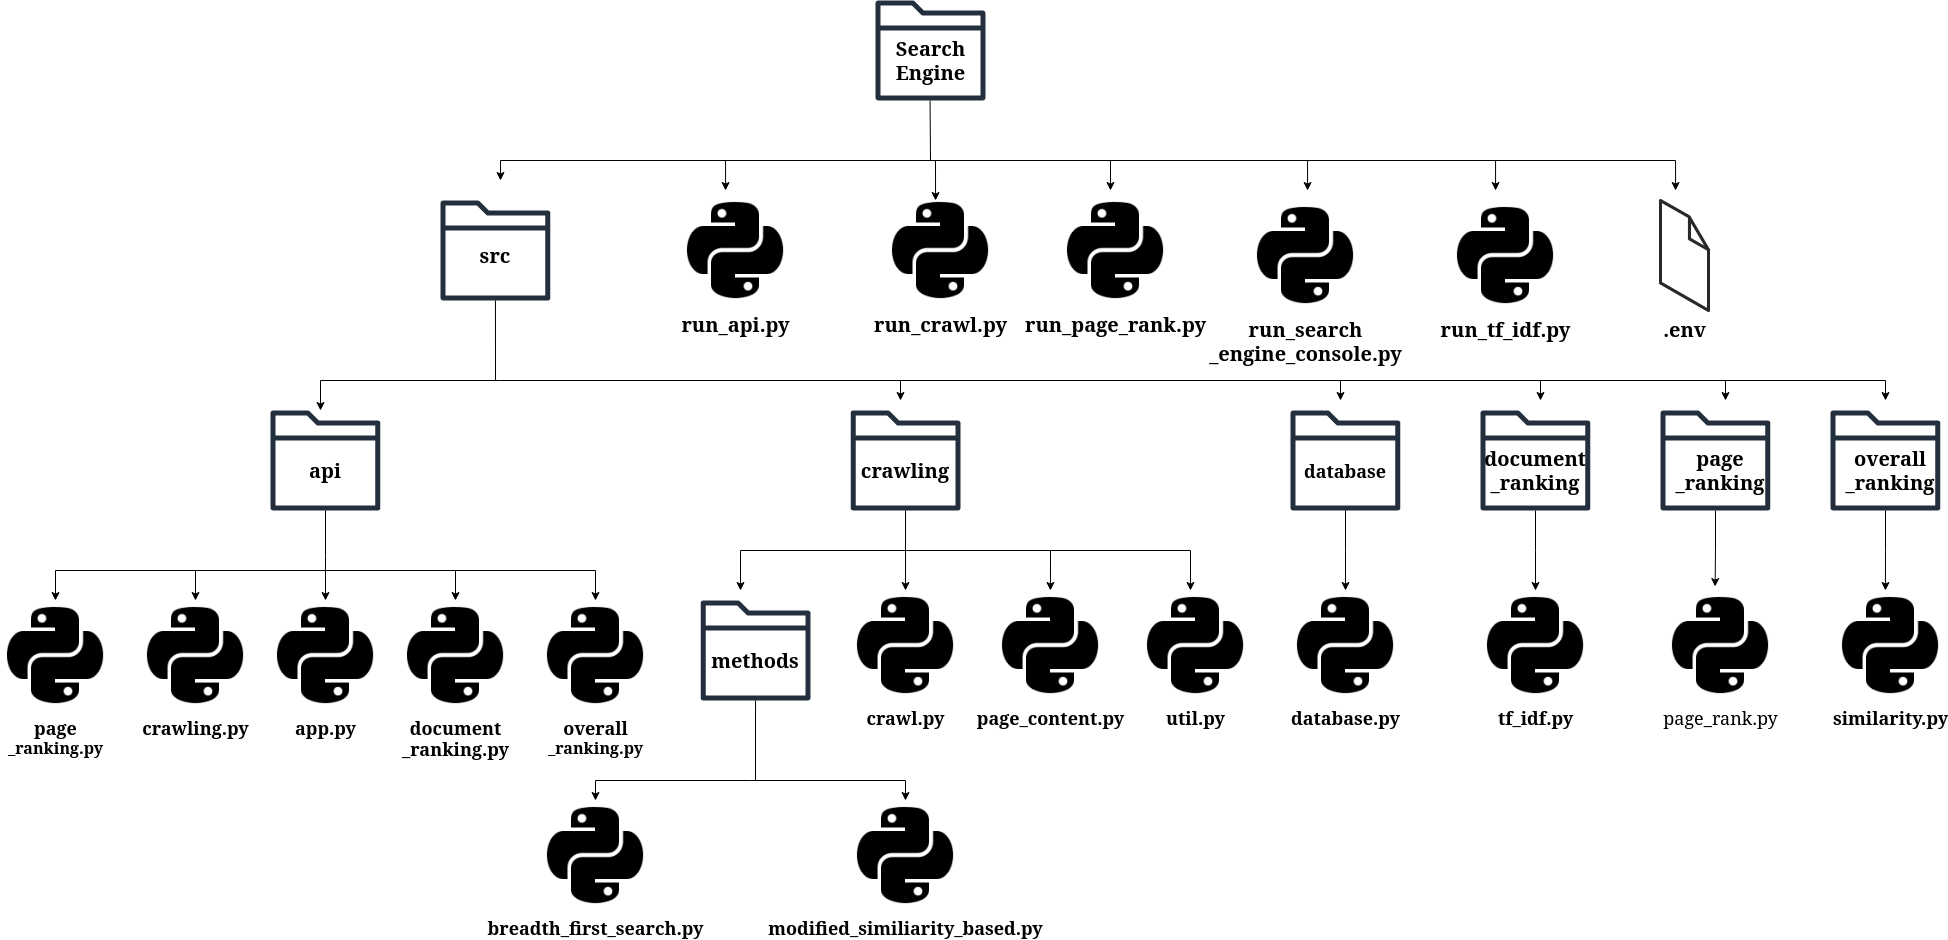
\includegraphics[keepaspectratio, width=14.5cm]{gambar/diagram-new.png}
  \caption{\emph{Struktur file \emph{search engine} Lazuardi} \citep{lazuardithesis}}
	\label{gambar:google_architecture}
\end{figure}

Proses \emph{crawling} dalam arsitektur \emph{Search engine} milik lazuard memiliki beberapa tahap, Tahap awal adalah \emph{crawler} akan mengakses \emph{origin url} yang disediakan dalam \emph{environment variable}. Untuk melakukan proses \emph{crawling}, perlu untuk menginisiasikan beberapa data yang akan digunakan dalam proses crawling seperti \emph{origin url} yang akan di akses, maksimum \emph{os threads} yang akan digunakan oleh crawler, dan durasi proses \emph{crawling}. Proses pertama yang dilakukan oleh \emph{crawler} setelah di inisiasi adalah dengan melakukan pengecekan ke \emph{database} apakah terdapat page yang sudah di \emph{crawl} atau belum, bila sudah maka crawler akan memulai proses \emph{crawling} dari page terakhir yang sebelumnya telah di \emph{parse}. Bila tidak, maka proses \emph{crawling} akan dimulai dari \emph{origin url}. List dari origin url akan dimasukkan kedalam \emph{queue} yang nantinya akan digunakan oleh proses \emph{Breadth First Search} dalam \emph{crawler}. Sebelum proses parse dilakukan data-data yang berhubungan dengan \emph{page} yang akan di \emph{parse} akan di insert kedalam database, seperti \emph{string url} dan duration \emph{parse}. Proses parsing page dilakukan menggunakan algoritma \emph{Breadth First Search}. Dalam menjalankan \emph{Breadth First Search}, setiap \emph{instance} \emph{page scrapper} dijalankan secara paralel didalam \emph{thread process}. \emph{Page scrapper} akan melakukan parsing tiap \emph{page} yang diakses dan mengambil beberapa bagian data dari  \emph{page} tersebut. Data yang parse dari \emph{page} merupakan data penting yang berisi inti sari dari \emph{page} tersebut dan data lain yang akan mendukung proses \emph{crawling} dan proses-proses selanjutnya dalam arsitektur \emph{search engine}, beberapa data yang diambil oleh \emph{scrapper} adalah \emph{article body} dari \emph{html page}, \emph{meta description} dari \emph{page}, \emph{meta keyword}, \emph{css page style} dari page, \emph{script} yang di \emph{embedded} dalam page, \emph{list}, \emph{form}, \emph{table}, \emph{image} dalam \emph{page}, dan \emph{hyperlink} yang ada di \emph{page} tersebut. Data-data yang telah dikumpulkan tersebut akan di masukkan ke dalam \emph{database} \citep{lazuardithesis}.

Dalam proses \emph{crawling} setiap kali \emph{page scrapper} selesai dalam menjelajahi dan melakukan \emph{parsing} dalam satu page, \emph{page scrapper} akan memasukkan url list yang di dapat dari dalam page kedalam \emph{queue}. Agar proses penambahan link kedalam queue tidak terganggu, penambahan \emph{queue} dilakukan secara \emph{syncronous} menggunakan lock. \emph{Url list} yang disimpan di dalam \emph{queue} ini nantinya akan di akses oleh \emph{page scrapper} lain. Proses ini akan berlanjut terus secara paralel dan pengaksesan tiap-tiap url dilakukan menggunakan algoritma \emph{breadth first search} \citep{lazuardithesis}.

\subsection{\emph{Breadth First Search}}

Untuk menjelajahi \emph{url list} yang ada di dalam \emph{queue} \emph{crawler} menggunakan algoritma \emph{breadth first search}, algoritma ini pada dasarnya merupakan algoritma untuk menjelajahi \emph{graph} dalam suatu \emph{tree}. Dalam penerapannya di dalam arsitektur \emph{search engine} milik lazuardi \emph{breadth first search} dimanfaatkan dalam proses pemilihan url yang akan diakses dalam setiap iterasi proses \emph{page scrapping} \citep{lazuardithesis}. Dalam menjelajahi \emph{tree}, algoritma ini menggunakan struktur data \emph{queue} untuk menyimpan informasi tentang \emph{node} yang akan dijelajahi selanjutnya dan \emph{stack} untuk menyimpan informasi mengenai \emph{node} yang telah di jelajahi. Metode \emph{breadth first search} memungkinkan untuk \emph{crawler} memprioritaskan penjelajahan \emph{url} yang telah dimasukkan ke dalam \emph{queue} terlebih dahulu, hal ini menjamin agar setiap tingkatan \emph{node} sudah dijelajahi sebelum lanjut ke tingkat \emph{node} selanjutnya \citep{cormen2009introduction}.

\begin{algorithm}[H]
	\caption{\emph{BFS($G,s$)} \citep{cormen2009introduction}}
	\label{algoritma_bfs}
	\begin{algorithmic}[1]
		\For{each vertex $u \in G.V - \{s\}$}
		\State $ u.color =$ WHITE
		\State $ u.d = \infty$
		\State $ u.\pi =$ NIL
		\EndFor
		\State $ s.color = $ GRAY
		\State $s.d = 0$
		\State $s.\pi = NIL$
		\State $Q = \infty$
		\State ENQUEUE($Q,s$)
		\While{$Q\not=\emptyset$}
		\State $u =$ DEQUEUE(Q)
		\For{each $v \in G.Adj[u]$}
		\If{$v.color ==$ WHITE}
		\State $v.color ==$ GRAY
		\State $v.d = u.d +1$
		\State $v.\pi = u$
		\State ENQUEUE($Q, v$)
		\State $v.color ==$ BLACK
		\EndIf
		\EndFor
		\EndWhile
	\end{algorithmic}
\end{algorithm}

Dalam arsitektur \emph{search engine} milik Lazuardi algoritma \emph{breadth first search} didefinisikan di dalam \emph{class BreadthFirstSearch}, \emph{class} ini terletak di dalam file \url{breadth_first_search.py}. Di dalam penerapan algoritma \emph{breadth first search} pada arsitektur \emph{search engine} milik lazuardi proses jalannya algoritma \emph{breadth first search} dibagi menjadi dua tahap, proses yang berjalan di dalam \emph{main thread} dan proses yang berjalan di dalam individual \emph{thread} yang sudah di \emph{spawn}. Contoh penerapan \emph{breadth first search} dalam arsitektur lazuardi dapat dilihat pada \ref{gambar:bfs_python} \citep{lazuardithesis}.

\begin{figure}[H]
	\centering
	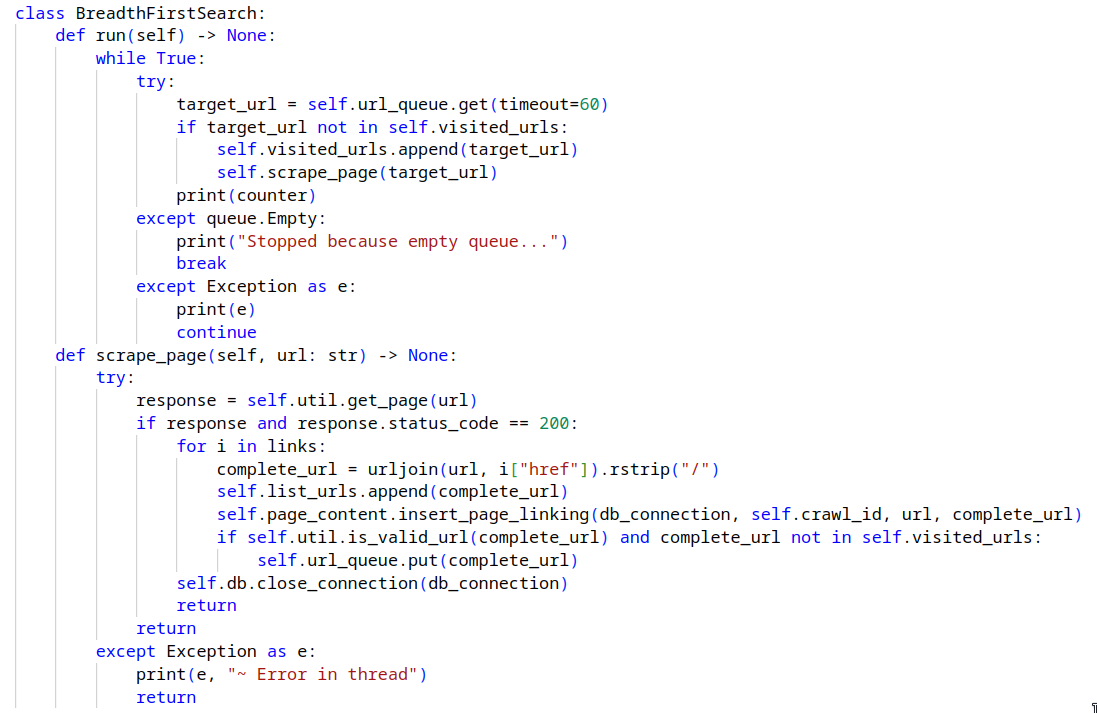
\includegraphics[keepaspectratio, width=15cm]{gambar/bfs-python.png}
  \caption{Algoritma \emph{breadth first search} dalam arsitektur lazuardi \citep{lazuardithesis}}
	\label{gambar:bfs_python} 
\end{figure}

Jalannya \emph{breadth first search} di arsitektur milik lazuardi dimulai dengan mengambil list \emph{url} dari \emph{queue} yang ada ke dalam variabel \emph{target\_url}, setelah itu dilakukan pengecekkan terhadap \emph{url} tersebut pada \emph{visited\_url} yang ada didalam \emph{stack}, bila \emph{url} itu belum pernah dikunjungin maka \emph{url} tersebut akan di marked sebagai \emph{visited url}. \emph{Url} yang telah di tandai akan di proses di dalam fungsi \emph{scrape\_page}, di dalam fungsi ini \emph{url} yang diterima akan di akses dan di \emph{parse}. Salah satu target pencarian dari proses \emph{parsing} page adalah \emph{url} page lain yang ditanam di dalam \emph{page} tersebut, \emph{url} tersebut akan di masukkan kedalam \emph{array} dan \emph{queue crawler} \citep{lazuardithesis}. Algoritma ini menggunakan struktur data \emph{queue} yang menggunakan prinsip \emph{First In First Out}, hal ini menyebabkan data atau dalam skenario ini \emph{url} yang terlebih dahulu diambil oleh crawler merupakan \emph{url} yang dimasukkan lebih awal, mekanisme ini mendukung agar algoritma dapat menjelajahi tiap-tiap level \emph{tree} secara menyeluruh sebelum pindah ke level \emph{tree} yang lebih dalam \citep{cormen2009introduction}. 

\begin{figure}[H]
	\centering
	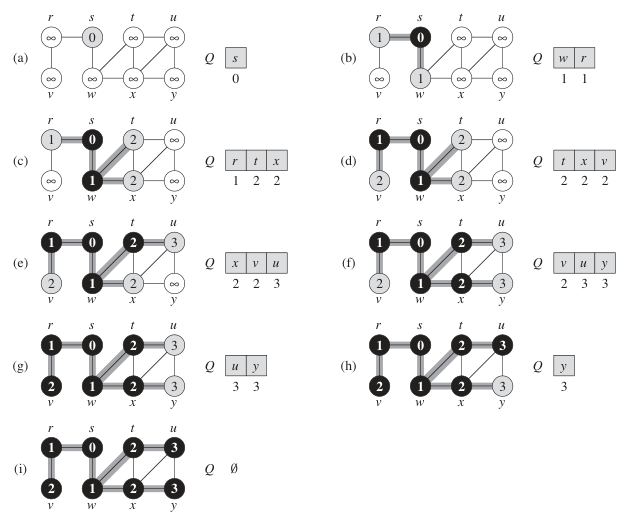
\includegraphics[keepaspectratio, width=10cm]{gambar/bfs-diagram.png}
  \caption{\emph{Diagram alur algoritma \emph{breadth first search} \citep{cormen2009introduction}}}
	\label{gambar:bfs_diagram} 
\end{figure}

\subsection{\emph{Threading}}

Untuk menjalankan algoritma \emph{breadth first search} proses \emph{page scrapping} secara efisien, arsitektur \emph{search engine} lazuradi memanfaatkan proses \emph{multi-thread}. Thread merupakan bagian terkecil dari suatu proses yang berjalan secara berurutan yang dapat dijalankan dan dikelola oleh \emph{cpu scheduler} dan pada dasarnya hanya terdapat satu proses yang dapat berjalan dalam satu thread \citep{operatingsystemconcept}. Arsitektur \emph{search engine} milik lazuardi memanfaatkan \emph{thread} untuk mengisolasi setiap proses \emph{page scrapping} dan menjalankannya secara paralel, hal ini memungkinkan untuk tiap-tiap instance dari \emph{page scrapper} untuk berjalan secara independen dalam melakukan penjelajahan dan \emph{parsing} dari halaman \emph{website}.

\begin{figure}[H]
	\centering
	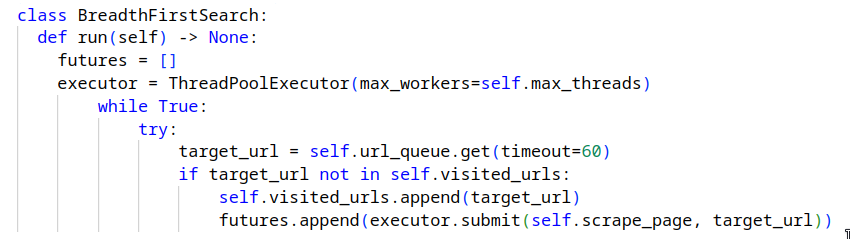
\includegraphics[keepaspectratio, width=15cm]{gambar/threading-python.png}
  \caption{Algoritma \emph{multi threading} dalam arsitektur lazuardi \citep{lazuardithesis}}
	\label{gambar:threading_python} 
\end{figure}
 
Proses \emph{threading} dalam arsitektur \emph{search engine} lazuardi dimulai dengan pengalokasian jumlah \emph{thread} maksimum yang dapat di gunakan oleh proses \emph{page scrapping}, jumlah maksimum thread ini dapat diatur sesuai dengan kapasitas \emph{cpu} mesin dan berapa banyak halaman \emph{web} yang akan di \emph{crawl}, proses pengalokasian jumlah maksimum \emph{thread} ini dilakukan menggunakan \emph{ThreadPoolExecutor}. \emph{ThreadPoolExecutor} merupakan \emph{class} dari \emph{python} yang berfungsi untuk mengatur pengalokasian beberapa jumlah \emph{thread} secara otomatis, ini mempermudah proses alokasi sumber daya \emph{thread} untuk proses yang ditentukan dengan jumlah \emph{thread} yang telah ditentukan. \emph{Thread pool} yang telah diinisiasi selanjutnya digunakan untuk menjalankan fungsi \emph{scrape\_page} yang sudah didefinisikan sebelumnya, hal ini agar setiap jalannya fungsionalitas \emph{page scrapper} berjalan diatas satu \emph{thread process}. Dengan menggunakan \emph{thread} proses \emph{scraping} dapat berjalan secara \emph{asyncronous} dan penjelajahan tiap-tiap halaman \emph{website} berjalan lebih cepat \citep{lazuardithesis}.

\subsection{\emph{Parsing} Halaman \emph{website} dan penyimpanan data}

Dalam jalannya proses algoritma \emph{breadth first search} yang sudah dijelaskan sebelumnya terdapat satu proses yang dinamakan \emph{page scrapping}. Proses ini bertujuan untuk mengekstraksi data penting dari halaman \emph{website} yang sedang di kunjungi oleh \emph{crawler}, data - data ini dikumpulkan ini lah yang nantinya akan digunakan untuk proses - proses selanjutnya dalam alur arsitektur \emph{search engine} milik lazuardi. Dalam arsitektur \emph{search engine} milik lazuardi proses ini di lakukan dengan menggunakan bantuan library \emph{beautifulsoup4} \citep{lazuardithesis}. Dalam implementasi arsitektur \emph{search engine} milik lazuardi proses \emph{page scrapping} dilakukan didalam setiap satu \emph{thread} yang telah dibuat sebelumnya dan satu proses \emph{page scrapping} akan berjalan pada satu halaman \emph{website}, hal ini dilakukan untuk menjamin jalannya proses \emph{page scrapping} berjalan dengan cepat. Informasi yang di ambil dari proses \emph{page scrapping} akan di bagi kedalam beberapa kategori, tujuannya untuk menjaga konsistensi data dan mempermudah proses selanjutnya dalam melakukan pengambilan data \citep{lazuardithesis}.

  \begin{center}
    \begin{longtable}{ |p{1cm}|p{3cm}|p{7cm}| }
      \caption{\emph{HTML Tag} dari halaman \emph{web} yang di ambil oleh \emph{crawler} \citep{lazuardithesis}} \\

      \hline \textbf{no}.& \textbf{tag}& \textbf{deskripsi} \\ \hline
      \endfirsthead

      \hline \textbf{no}.& \textbf{tag}& \textbf{deskripsi} \\ \hline
      \endhead

      \hline \multicolumn{3}{r}{{Dilanjutkan pada halaman berikutnya}} \\
      \endfoot

      \hline \hline
      \endlastfoot

      1& \emph{body/article}& konten utama \\ \hline
      2& \emph{meta description}& Deskripsi singkat dari halaman web \\ \hline
      3& \emph{meta keyword}& Kata kunci yang merepresentasikan isi halaman web \\ \hline
      4& \emph{style}& \emph{css style} dalam suatu halaman web \\ \hline
      5& \emph{list}& isi dari \emph{list} yang terdapat dalam halaman web \\ \hline
      6& \emph{form}& form dan input yang terdapat dalam halaman web \\ \hline
      7& \emph{table}& kumpulan elemen \emph{table} dalam halaman web \\ \hline
      8& \emph{image}& kumpulan \emph{url} yang mengarah pada gambar di halaman web \\ \hline
      9& \emph{outgoing link}& kumpulan \emph{url} referensi yang mengarah pada halaman web lain \\ \hline
    \end{longtable}
  \end{center}

  Data-data yang telah dikelompokkan ini selanjutnya akan dimasukkan ke dalam \emph{database} yang sudah disiapkan. Struktur data dari \emph{database} akan mencerminkan permbagian kategori data yang didapatkan seperti Tabel 2.1. Gambar \ref{gambar:lazuardy_database} merupakan struktur \emph{database} yang digunakan oleh arsitektur \emph{search engine} lazuardy \citep{lazuardithesis}.

\begin{figure}[H]
	\centering
	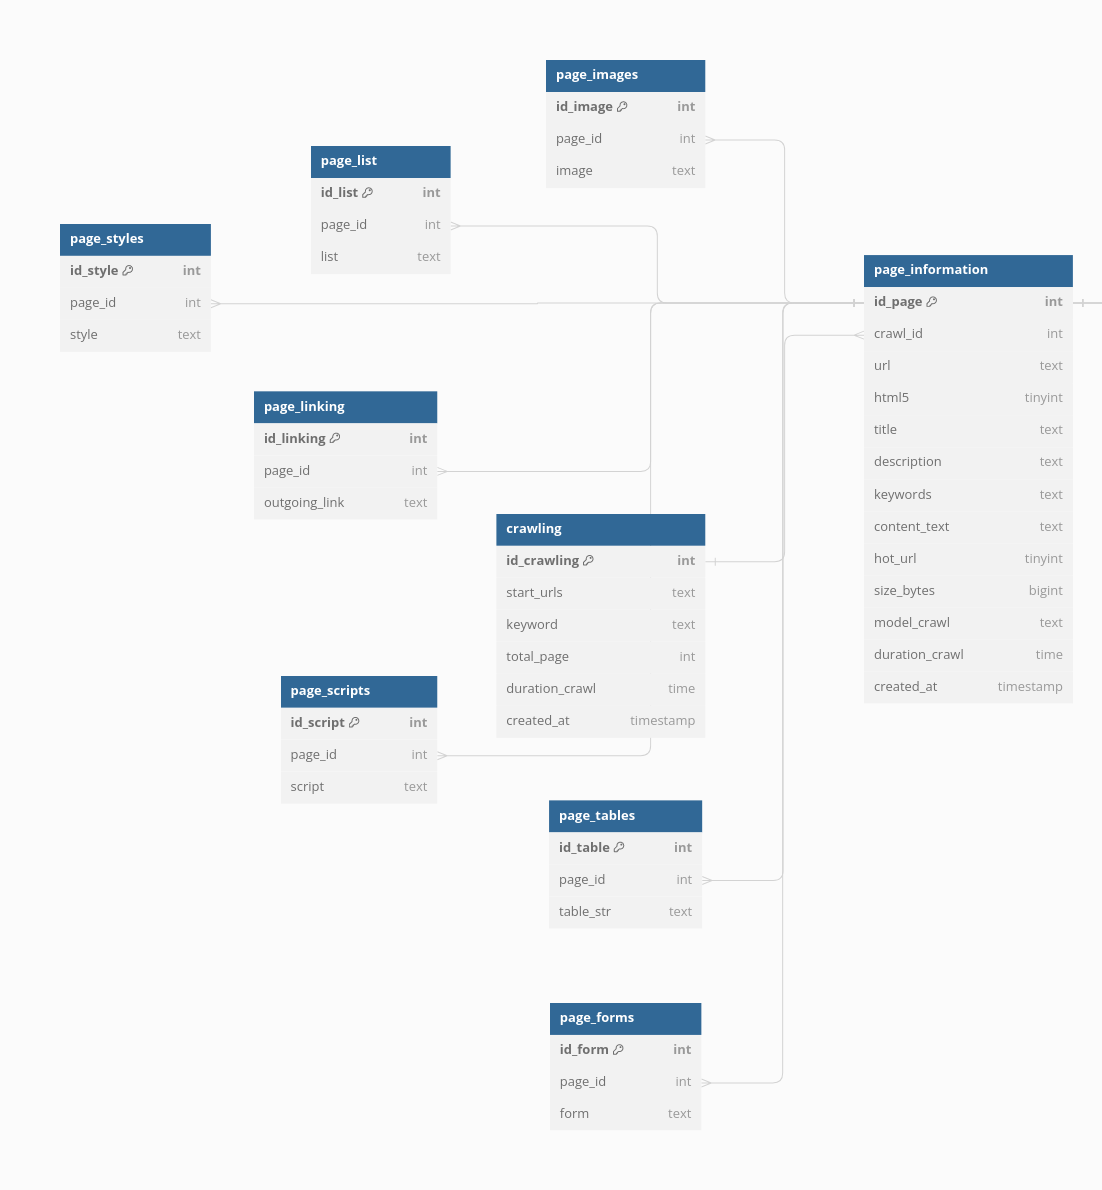
\includegraphics[keepaspectratio, width=14.5cm]{gambar/crawler-erd.png}
  \caption{\emph{Entity Relations Diagram} database lazuardi \citep{lazuardithesis}}
	\label{gambar:lazuardy_database}
\end{figure}

\subsection{\emph{Library} dalam arsitektur \emph{search engine} Lazuardy}

Arsitektur \emph{search engine} milik lazuardy dikembangkan menggunakan platform bahasa pemograman \emph{python} dengan menggunakan \emph{runtime cpython} versi 3.0. Untuk menjalankan fungsionalitas \emph{search engine} terdapat penggunaan berbagai \emph{standard library} dan \emph{third-pary library} dalam menjalankan proses tertentu seperti pengambilan data dari halaman web sampai penyimpanan data ke dalam \emph{database}. \emph{Standard library} dari \emph{python} yang digunakan dalam arsitektur ini adalah \emph{queue}, \emph{time}, \emph{threading}, \emph{os}, \emph{regex} dan, \emph{request} \citep{lazuardithesis}.

  \begin{center}
    \begin{longtable}{ |p{1cm}|p{4cm}|p{5cm}| }
      \caption{Daftar \emph{library} yang digunakan dalam arsitektur \emph{search engine} milik lazuardy \citep{lazuardithesis}} \\ \hline

      \multicolumn{3}{|c|}{Daftar \emph{library} \emph{third party}} \\ \hline
      \endfirsthead

      \hline \multicolumn{3}{|c|}{Daftar \emph{library} \emph{third party}} \\ \hline
      \endhead

      \hline \multicolumn{3}{r}{{Dilanjutkan pada halaman berikutnya}} \\
      \endfoot

      % Last footer without next page indication
      \hline \hline
      \endlastfoot

      No.& Nama \emph{library}& Fungsi \\ \hline
      1.& \emph{beautifulsoup4}& Parsing menyusun \emph{language tree} untuk mengambil informasi \\ \hline
      2.& \emph{requests}& Melakukan \emph{request} untuk mengunduh halaman \emph{website} \\ \hline
      3.& \emph{pandas}& Melakukan interaksi dengan matriks \\ \hline
      4.& \emph{pymysql}& \emph{Interface} untuk melakukan operasi \emph{query} \\ \hline
      5.& \emph{python-dotenv}& Mengambil data dari \emph{environtment variable} \\ \hline
      6.& \emph{psutil}& Melakukan \emph{monitoring} dan pengambilan informasi dari \emph{process} \emph{python} yang berjalan \\ \hline
      7.& \emph{scikit-learn}& Membuat model perhitungan \emph{TF-IDF} \\ \hline
      8.& \emph{numpy}& Melakukan perhitungan matematika kompleks \\ \hline
      9.& \emph{pdoc3}& Penulisan Dokumentasi \\ \hline
      10.& \emph{flask}& Penyediaan \emph{API} \emph{server} untuk antarmuka operasi \emph{search engine} \\ \hline
    \end{longtable}
  \end{center}

\section{\emph{Process dan Threads}}

Pada awalnya komputer generasi awal hanya bisa menjalankan satu program pada satu waktu, program ini memiliki akses penuh terhadap semua \emph{resources} pada komputer. Keterbatasan komputer generasi awal ini membuat hal yang dapat dilakukan di komputer menjadi sangat terbatas, berbeda komputer generasi awal komputer generasi sekarang dapat menjalankan beberapa program secara bersamaan. Hal ini didukung dengan arsitektur komputer yang \emph{multi-core} dan kapasitas \emph{memory} yang lebih besar. Dengan banyaknya penggunaan komputer dengan jumlah \emph{core} yang banyak, mekanisme agar komputer dapat menjalankan beberapa program sekaligus semakin dibutuhkan. Komputer \emph{modern} memiliki mekanisme yang dapat digunakan agar beberapa program dapat di muat kedalam \emph{memory} dan dijalankan secara bersamaan, terdapat dua metode yang dapat mendukung jalannya mekansime ini, yaitu \emph{process} dan \emph{threads} \citep{operatingsystemconcept}.

\subsection{\emph{Process}}

\emph{Process} pada dasarnya adalah \emph{program} yang sedang dijalankan oleh komputer, \emph{program} pada sendirinya hanya file pasif yang berisi instruksi - instruksi yang perlu dijalankan oleh komputer. Instruksi tersebut yang menjadi satu \emph{instance} dari \emph{process}. \emph{Process} mengakses data yang diperlukan untuk proses komputasi dari \emph{virtual memory}, data di dalam memory ini bersifat sementara dan disimpan sebagai \emph{cache}. \emph{Memory} yang dapat diakses oleh \emph{process} memiliki susunan tertentu yang terbagi menjadi beberapa bagian.
\begin{figure}[H]
	\centering
	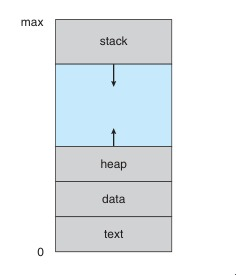
\includegraphics[keepaspectratio, width=6cm]{gambar/memory-layout.jpeg}
  \caption{Susunan bagian dari \emph{virtual memory} \citep{operatingsystemconcept}}
	\label{gambar:memory_layout}
\end{figure}

Dari gambar \ref{gambar:memory_layout} dapat dilihat bahwa susunan \emph{vitual memory} yang dapat diakses oleh \emph{process} yang berjalan terbagi menjadi beberapa bagian yang dibagi berdasarkan jenis data yang disimpan dan tingkat alamat dari data tersebut dalam \emph{memory} \citep{operatingsystemconcept}. Bagian-bagian dalam \emph{virtual memory} adalah,

\begin{enumerate}
  \item \emph{Text}. Data yang berisi kode yang dijalankan
  \item \emph{Data}. Data yang berisi variabel global dalam kode
  \item \emph{Heap}. Sejumlah Ukuran \emph{memory} yang dialkokasikan secara dinamis oleh program saat program sedang berjalan atau \emph{runtime}
  \item \emph{Stack}. Penyimpanan data sementara yang disediakan saat pemanggilan fungsi dalam kode.
\end{enumerate}

Ukuran dari bagian \emph{text} dan \emph{data} dalam memory adalah tetap, sedangkan ukuran \emph{heap} dan \emph{stack} dapat bertambah dan berkurang secara dinamis saat \emph{process} sedang berjalan. Walaupun \emph{program} atau kode dapat membuat dua \emph{process} yang berbeda, setiap \emph{process} tersebut memiliki blok \emph{virtual memory} masing-masing dengan data dalam bagian \emph{text} yang sama dan bagian lain seperti \emph{data}, \emph{heap}, dan \emph{stack} yang berbeda sesuai dengan instruksi yang diajalankan pada setiap \emph{process} \citep{operatingsystemconcept}.

Saat \emph{process} berjalan, \emph{process} akan mengubah \emph{state}. \emph{State} adalah indikasi status dari \emph{process} terkait yang sedang berjalan. State dari \emph{process} akan berubah ketika terdapat operasi yang dilakukan terhadap \emph{process} terkait, nama dan alur dari perubahan \emph{state} ini berbeda di setiap \emph{operating system} tetapi konsep dari \emph{process state} ini dapat ditemukan di semua \emph{operating system} \citep{operatingsystemconcept}.

\begin{figure}[H]
	\centering
	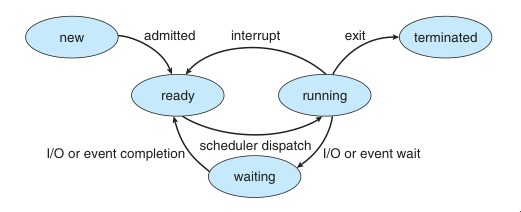
\includegraphics[keepaspectratio, width=12cm]{gambar/state-process.jpeg}
  \caption{Alur perubahan dari \emph{process state} \citep{operatingsystemconcept}}
	\label{gambar:state_process_flow}
\end{figure}

Dari gambar \ref{gambar:state_process_flow} dapat dilihat alur perubahan dari \emph{process state} dan \emph{event} apa yang dapat memicu perubahan \emph{process state} tersebut. Perlu diketahui gambar \ref{gambar:state_process_flow} tidak menampilkan perubahan \emph{process state} yang spesifik dari \emph{operating system} tertentu, tetapi \emph{state} yang dari figur tersebut dapat ditemui di seluruh \emph{operating system} \citep{operatingsystemconcept}. \emph{State} yang ada di gambar \ref{gambar:state_process_flow} adalah,

\begin{enumerate}
  \item{\emph{New}. \emph{Process} baru yang dibuat}
  \item{\emph{Running}. Instruksi yang sedang di eksekusi}
  \item{\emph{Waiting}. \emph{Process} yang sedang menunggu \emph{trigger event}}
  \item{\emph{Ready}. \emph{Process} yang menunggu alokasi \emph{processor}}
\end{enumerate}

\subsection{\emph{Inter-process Communication}}

Beberapa \emph{process} yang dijalankan secara bersamaan oleh \emph{operating system} dapat dibagi menjadi dua kategori \emph{process} yang berjalan sendiri dan tidak berkaitan dengan \emph{process} lain, dan \emph{process} yang jalannya berkaitan dengan \emph{process} lain. \emph{Process} yang mekanismenya berkaitan dengan \emph{process} lain perlu strategi dan mekanisme dalam berbagi data dengan \emph{process}, hal ini dapat disebut  dengan \emph{inter-process communication} \citep{operatingsystemconcept}.

Terdapat 2 mekanisme dasar \emph{inter-process communication} yaitu mekanisme \emph{shared memory} dan \emph{message passing}. Dalam mekanisme \emph{shared memory} terdapat bagian dari \emph{virtual memory} yang di digunakan secara bersamaan oleh 2 \emph{process} yang berkaitan, dengan metode ini kedua \emph{process} akan menulis dan mengambil data dari bagian \emph{virtual memory} yang sama. Dalam metode \emph{message passing} data yang dikomunikasikan melalui pertukaran pesan antara dua \emph{process} \citep{operatingsystemconcept}. 

\begin{figure}[H]
  \centering
	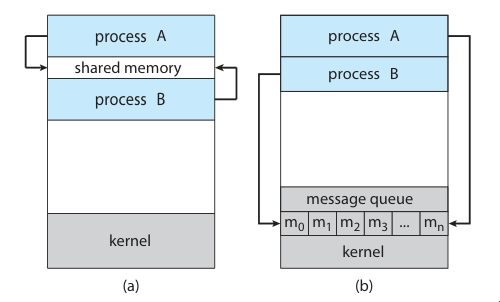
\includegraphics[keepaspectratio, width=12cm]{gambar/ipc_models.png}
  \caption{Metode komunikasi antar \emph{process}. (a) \emph{Shared memory}. (b) \emph{Message passing} \citep{operatingsystemconcept}}
	\label{gambar:ipc_models}
\end{figure}

Selain 2 metode yang sudah dijelaskan sebelumnya juga terdapat metode \emph{inter-process communication} yang lebih berfokus pada komunikasi pada sistem \emph{client-server}, salah satu metodenya adalah \emph{socket}. \emph{Socket} secara definisi merupakan metode komunikasi antar proses yang dikirimkan dengan format tertentu kepada alamat tertentu. \emph{Socket} sendiri terbagi menjadi dua jenis, yaitu \emph{network socket} yang dapat digunakan dua perangkat berbeda untuk berkomunikasi dengan perantara jaringan internet dan \emph{UNIX domain socket} yang hanya dapat digunakan oleh komunikasi antar proses dalam perangkat yang sama dengan sistem operasi yang bersifat \emph{POSIX compliant} \citep{operatingsystemconcept}.

\subsection{\emph{Threads}}

\emph{Process} dapat di jelaskan sebagai \emph{program} yang dijalankan dalam satu \emph{threads} yang berjalan, contoh dari konsep ini adalah ketika \emph{program} pengolah kata sedang dijalankan instruksi-instruksi yang ada pada \emph{program} dijalankan secara berurutan dalam satu \emph{thread} yang berjalan. \emph{Thread} memungkinkan untuk \emph{process} untuk menjalankan satu \emph{instruction} dalam satu waktu dan membuat jalan dari keseluruhan \emph{instruction} dalam \emph{program} untuk berjalan secara berurutan. Dalam \emph{operating system} modern konsep dari \emph{thread} ini ditingkatkan sehinggan satu \emph{process} dapat menjalankan beberapa \emph{thread} secara bersamaaan sehingga lebih dari satu \emph{instruksi} dapat dijalankan secara bersamaan \citep{operatingsystemconcept}. 

\begin{figure}[H]
  \centering
	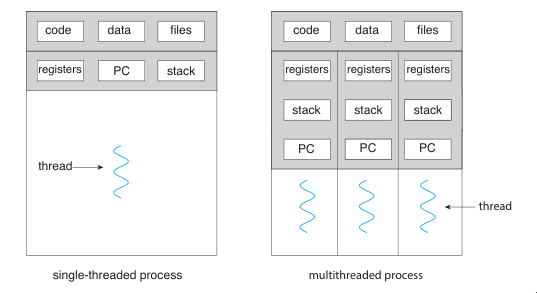
\includegraphics[keepaspectratio, width=12cm]{gambar/thread_process.png}
  \caption{\emph{Process} dengan satu \emph{thread} dan lebih dari satu \emph{thread} \citep{operatingsystemconcept}}
	\label{gambar:thread_process}
\end{figure}

Dalam gambar \ref{gambar:thread_process} terlihat bahwa beberapa \emph{thread} yang berjalan secara bersamaan dalam satu \emph{process} yang sama pada dasarnya berbagi \emph{resources} seperti \emph{virtual memory} yang sama. Hal ini memungkinkan dalam jalannya satu \emph{program} beberapa instruksi dengan \emph{performance cost} yang besar untuk dilankan secara bersamaan dengan proses sinkronisasi data yang lebih mulus, selain itu proses locking antar \emph{thread} akan lebih mudah dikelola dengan adanya \emph{virtual memory} yang sama antar \emph{thread} \citep{operatingsystemconcept}. 

Mekanisme pembuatan dan jalannya \emph{thread} bergantung dengan sistem operasi yang digunakan dalam perangkat. Dalam sistem operasi \emph{windows} aplikasi berjalan diatas \emph{process} dan tiap \emph{process} terdiri dari satu atau lebih \emph{thread}, \emph{windows} menggunakan strategi \emph{one to one mapping} dalam manajemen \emph{thread}-nya dimana \emph{thread} dibagi menjadi dua jenis yaitu \emph{thread} yang berjalan di dalam \emph{user space} dan \emph{kernel space}. Setiap \emph{thread} dalam \emph{user space} dipetakan ke \emph{thread kernel} yang terkait. Dalam \emph{windows} pembagian jenis \emph{thread} terlihat dengan jelas dan memiliki struktur data yang pasti. Terdapat 3 struktur data \emph{thread} dalam windows yaitu \emph{ETHREAD} atau \emph{executive thread block}, \emph{KTHREAD} atau \emph{kernel thread block}, dan \emph{TEB} atau \emph{therad environment block} \citep{operatingsystemconcept}.

\begin{figure}[H]
  \centering
	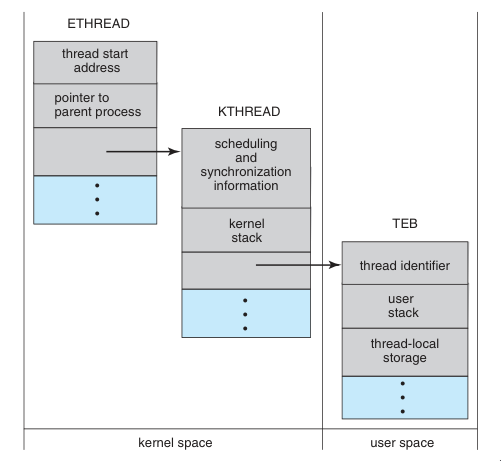
\includegraphics[keepaspectratio, width=10cm]{gambar/windows-thread.png}
  \caption{Struktur data dari \emph{windows thread} \citep{operatingsystemconcept}}
	\label{gambar:windows_thread}
\end{figure}

Berbeda dengan \emph{window}, pembagian jenis \emph{thread} dalam sistem operasi \emph{linux} tidak terlihat dengan jelas. \emph{Linux} menyediakan dua \emph{system call} untuk berinteraksi dengan pembuatan \emph{process} dan \emph{thread} yaitu \emph{fork()} dan \emph{clone()}, tetapi \emph{linux} tidak membedakan secara spesifik antara \emph{thread} dan \emph{process}. Perbedaan antara \emph{thread} dan \emph{process} dalam \emph{linux} terlihat dari seberapa banyak pembagian data yang terjadi diantara tiap-tiap \emph{task}, pembagian ini dideklarasikan ketika \emph{system call} dipanggil dengan menambakan \emph{flags} tambahan \citep{operatingsystemconcept}.

\begin{figure}[H]
  \centering
	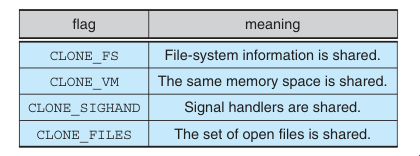
\includegraphics[keepaspectratio, width=10cm]{gambar/linux-thread.png}
  \caption{\emph{flags} yang dapat dipanggil \emph{clone()} \citep{operatingsystemconcept}}
	\label{gambar:linux_thread}
\end{figure}

Gambar \ref{gambar:linux_thread} merupakan \emph{flags} yang dapat dipanggil ketika memanngil \emph{system call} \emph{clone()}, setiap \emph{flags} memiliki tinkat pembagian \emph{resources} yang berbeda \citep{operatingsystemconcept}.

\section{\emph{Rust Programming Language}}

\emph{Rust programming language} merupakan bahasa pemograman level sistem dengan penekanan desain bahasa yang aman, dapat bekerja dengan konkuren dan cepat. \emph{Rust} sama seperti dengan bahasa pemograman sistem yang lain seperti \emph{C} atau \emph{C++} mengkompilasi kodenya menjadi \emph{machine code}, hal ini memberika dorongan kinerja yang lebih cepat terhadap hasil \emph{program} terhadap bahasa lain yang menggunakan mekanisme \emph{interpretation} seperti \emph{javascript} dan \emph{python} atau terhadap bahasa pemograman \emph{java} yang menggunakan \emph{virtual machine} untuk mentranslasi kode nya \citep{rustbook}. Layak nya bahasa pemograman sistem yang lain \emph{rust} menyediakan \emph{interface} untuk berinteraksi dengan abstraksi level rendah pada komputer seperti manajemen \emph{memory}, pengaturan terhadapa konkurensi dengan \emph{process} dan \emph{thread} dan akses terhadap \emph{API} dari \emph{operating system}. \emph{Rust} juga membawa konsep baru ke dalam dunia pemograman sistem dalam melakukan manajemen alokasi \emph{memory} dinamis di sistem, berbeda dengan bahasa pemograman \emph{C} dan \emph{C++} yang melakukan alokasi dan pelepasan \emph{space} pada memory bila sudah tidak digunakan secara manual \emph{rust} menggunakan sistem \emph{variable ownership} dan \emph{borrowing} ini memungkinkan \emph{rust} untuk tidak menggunakan \emph{garbage collector} dalam \emph{runtime} tetapi tetap menjaga keamanan \emph{memory}-nya \citep{rustbook}.

\subsection{Konsep Semantik Dari \emph{Ownership}}

Ketika \emph{program} ingin mengalokasikan ruang dalam \emph{memory} untuk menyimpan data yang dinamis bahasa pemograman harus mampu melakukan dua hal yaitu, mekanisme untuk mengalokasikan ruang dalam \emph{memory} untuk menyimpan data saat \emph{runtime} dan yang kedua adalah cara untuk melepas \emph{memory} tersebut kembali ke \emph{operating system} ketika data teresebut sudah tidak digunakan \citep{rustbook}. Bahasa pemograman dengan abstraksi level tinggi seperti \emph{python}, \emph{javascript}, \emph{go} dan \emph{java} menggunakan mekanisme \emph{garbage collection}, mekanisme ini memungkian agar \emph{program} untuk mengalokasikan ruang pada \emph{memory} ketika dibutuhkan dan melepas \emph{memory} ketika tidak dibutuhkan secara otomatis. Mekanisme \emph{garbage collection} dilakukan pada saat \emph{runtime} sehingga mempengaruhi performa dan waktu eksekusi dari program, ini membuat program yang dijalankan dengan mekanisme \emph{garbage collection} berjalan lebih lambat. Bahasa dengan abstraksi yang lebih rendah seperti \emph{C} dan \emph{C++} melakukan alokasi dan pelepasan ruang pada \emph{memory} secara manual, hal ini membuat \emph{program} yang dibuat rentan terhadap penggunaan \emph{memory} yang berlebihan atau data yang tidak valid ketika diakses. \emph{Rust} menggunakan sistem yang berbeda dari bahasa pemograman lain dalam mekanisme manajemen \emph{memory}, yaitu \emph{ownership} dan \emph{borowing} \citep{rustbook}

\emph{Ownership} adalah konsep manajemen \emph{memory} dalam \emph{rust} dengan konsep utama kepemilikan data oleh \emph{variable} \citep{rustbook}. Dalam mekanisme \emph{ownership} terdapat tiga aturan utama yaitu,

\begin{enumerate}
  \item{Setiap nilai atau \emph{value} memiliki \emph{variable} yang menjadi pemiliknya yang disebut \emph{owner}}
  \item{Setiap nilai hanya dapat memiliki \emph{owner} dalam satu waktu}
  \item{Ketika \emph{owner} dari nilai tersebut keluar dari cakupan, nilai nya akan dihapus}
\end{enumerate}

\emph{Rust} secara otomatis mengembalikan ruang yang dipakai di \emph{memory} oleh \emph{variable} yang sudah keluar dari jangkauan program. Keluar dari Jangkauan atau \emph{out of scope} adalah kondisi ketika \emph{variable} sudah tidak dapat digunakan atau di-akses \citep{rustbook}.
\begin{figure}[H]
  \centering
	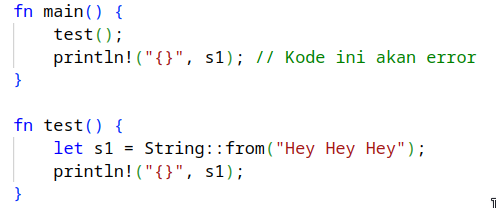
\includegraphics[keepaspectratio, width=12cm]{gambar/rust-scope.png}
  \caption{Scope dalam \emph{rust} \citep{rustbook}}
	\label{gambar:rust-scope}
\end{figure}

Dalam gambar \ref{gambar:rust-scope} terdapat dua \emph{function}, \emph{test()} dan \emph{main()}. Dalam fungsi \emph{test()} terdapat deklarasi \emph{variable} \emph{s1} berupa \emph{string}, data di-dalam \emph{s1} disimpan di-dalam \emph{heap} dan \emph{owner}-nya adalah \emph{s1}. Variabel \emph{s1} memiliki jangkauan hanya didalam \emph{test()}, ini artinya \emph{s1} tidak dapat di akses di luar fungsi \emph{test()} dan ini menjelaskan mengapa kode pada gambar \ref{gambar:rust-scope} akan error. Berbeda dengan bahasa pemograman lain, ketika variabel yang data-nya di simpan dalam \emph{heap} memiliki sifat-sifat yang unik dikarenakan pengaruh \emph{ownership} \citep{rustbook}.

\begin{figure}[H]
  \centering
	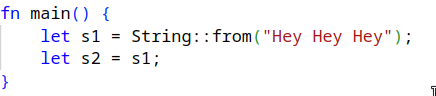
\includegraphics[keepaspectratio, width=12cm]{gambar/moving-data.png}
  \caption{Memindahkan data dari variabel \emph{s1} ke \emph{s2} \citep{rustbook}}
	\label{gambar:rust-data-transfer}
\end{figure}

\begin{figure}[H]
  \centering
	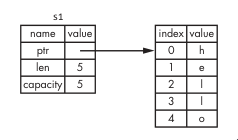
\includegraphics[keepaspectratio, width=7cm]{gambar/single-s1-memory.png}
  \caption{Representasi penyimpanan data dalam variabel \emph{s1} dalam \emph{memory} \citep{rustbook}}
	\label{gambar:single-memory-representation}
\end{figure}

\begin{figure}[H]
  \centering
	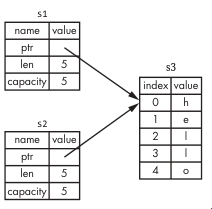
\includegraphics[keepaspectratio, width=7cm]{gambar/double-s1-s2-memory.png}
  \caption{Representasi penyimpanan data yang sama dalam dua variabel \emph{s1} dan \emph{s2} dalam \emph{memory} \citep{rustbook}}
	\label{gambar:double-memory-representation}
\end{figure}

Di kode dalam gambar \ref{gambar:rust-data-transfer} terlihat seperti data dari \emph{s1} di-\emph{copy} dan disimpan kedalam variabel \emph{s2}. Gambar \ref{gambar:single-memory-representation} merupakan representasi dalam \emph{memory} dari string yang disimpan dalam variabel \emph{s1}, tabel \emph{s1} dan tabel \emph{s2} merupakan data yang disimpan di dalam \emph{stack} dan berisi 3 komponen yaitu panjang dari \emph{string} tersebut, kapasitas maksimal dari \emph{string}, dan \emph{pointer} yang menunjuk ke lokasi di \emph{memory} yang menyimpan isi dari \emph{string} tersebut \citep{rustbook}. Tabel \emph{s3} merupakan isi sebenarnya dari \emph{string} tersebut yang disimpan di dalam \emph{heap}. Ketika variabel \emph{s1} disalin dan disimpan ke variabel baru, yang sebenarnya terjadi adalah data yang disalin hanya data dalam \emph{stack} saja dan data dalam variabel baru akan memiliki \emph{pointer} yang menunjuk ke lokasi \emph{heap} yang sama dengan data asli nya seperti yang terlihat di gambar \ref{gambar:double-memory-representation}. Ketika variabel keluar dari jangkauan \emph{program} \emph{rust} secara otomatis akan menghapus data variabel tersebut yang terdapat di dalam \emph{heap}, bila dalam skenario kode \ref{gambar:rust-data-transfer} kedua variabel \emph{s1} dan \emph{s2} keluar dari jangkauan program maka kedua variabel itu akan mencoba untuk menghapus data yang sama dalam \emph{memory}, hal ini disebut dengan nama \emph{double free error} yang merupakan permasalahan keamanan \emph{memory} yang \emph{rust} mencoba untuk tangani \citep{rustbook}.

\begin{figure}[H]
  \centering
	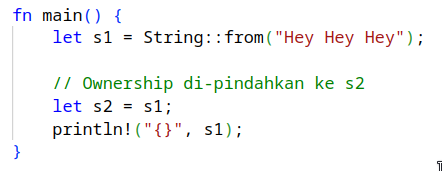
\includegraphics[keepaspectratio, width=12cm]{gambar/ownership-transfer.png}
  \caption{Memindahkan ownership dari variabel \emph{s1} ke \emph{s2} \citep{rustbook}}
	\label{gambar:rust-ownership-transfer}
\end{figure}

Untuk menghindari permasalahan keamanan yang terkait dengan \emph{double free error}, dalam kode \ref{gambar:rust-data-transfer} yang terjadi bukan hanya sekedar proses penyalinan \emph{memory} yang telah di alokasikan. Alih-alih hanya melakukan penyalinan, \emph{rust} akan menganggap \emph{s1} tidak lagi valid dan maka dari itu \emph{memory} yang berkaitan dengan \emph{s1} tidak perlu di hapus ketika \emph{s1} keluar dari jangkauan \emph{program} akibatnya, variabel \emph{s1} bila diakses setelah data-nya dipindahkan tidak akan berhasil \citep{rustbook}. Seperti yang terlihat di kode dalam gambar \ref{gambar:rust-ownership-transfer}, ketika \emph{s1} di-\emph{print} tidak akan berhasil.

Untuk melakukan proses penyalinan data dalam \emph{heap} yang tidak berbenturan dengan \emph{ownership}, \emph{rust} menyediakan metode \emph{clone}. \emph{Clone} merupakan metode penyalinan data yang berbasis dari konsep \emph{deep copy} ini berarti ketika metode ini dipanggil variabel kedua tidak hanya menyalin data dalam \emph{stack} saja namun juga menyalin data dalam \emph{heap} dari variabel tersebut, ini membuat metode \emph{clone} cocok untuk menyalin variabel yang data-nya disimpan didalam \emph{heap} seperti \emph{string} dan \emph{slice}. Kekurangan dari \emph{clone} adalah karena data dalam \emph{heap} juga disalin, jumlah \emph{memory} yang digunakan menjadi besar.\citep{rustbook}

\begin{figure}[H]
  \centering
	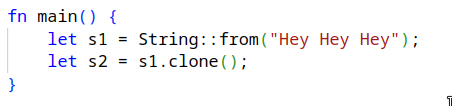
\includegraphics[keepaspectratio, width=12cm]{gambar/rust-clone-method.png}
  \caption{Penyalinan data \emph{s1} ke \emph{s2} \citep{rustbook}}
	\label{gambar:rust-clone-method}
\end{figure}

Ketika variabel diteruskan ke dalam \emph{function} secara semantik hal yang terjadi serupa dengan inisiasi data kedalam variabel. Meneruskan variabel kedalam \emph{function} akan memindahkan atau menyalin data seperti inisiasi variabel. Dalam kode \ref{gambar:rust-function-ownership} dapat dilihat contoh penggunaan \emph{function} dalam berinteraksi dengan \emph{ownership} dalam variabel \citep{rustbook}.

\begin{figure}[H]
  \centering
	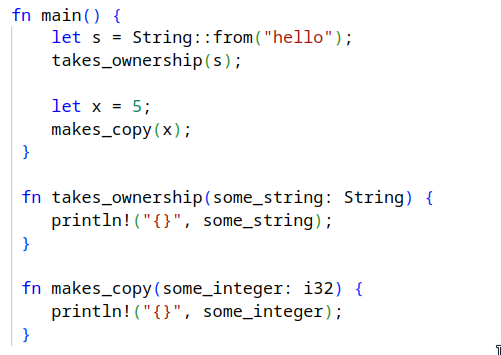
\includegraphics[keepaspectratio, width=12cm]{gambar/function-ownership.png}
  \caption{Penggunaan \emph{function} dengan \emph{ownership} \citep{rustbook}}
	\label{gambar:rust-function-ownership}
\end{figure}

Dalam kode \ref{gambar:rust-function-ownership} ketika \emph{function} mengambil parameter suatu variabel yang datanya berada di \emph{heap} dan variabel nya keluar cakupan dalam \emph{function} tersebut maka data-nya akan di hapus. Berbeda dengan ketika data yang tersimpan dalam \emph{stack} yang di lempar kedalam \emph{parameter} suatu \emph{function}, ketika variabel tersebut keluar jangkauan dalam \emph{function} tersebut tidak akan membuat variabel-nya terhapus \citep{rustbook}.

\begin{figure}[H]
  \centering
	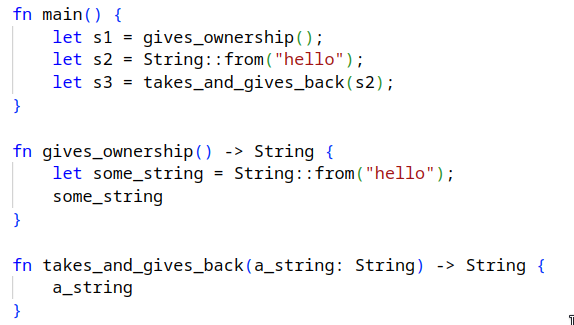
\includegraphics[keepaspectratio, width=12cm]{gambar/return-value-scope.png}
  \caption{Penggunaan \emph{function} dengan \emph{ownership} \citep{rustbook}}
	\label{gambar:rust-ownership-return}
\end{figure}

Dalam kode \ref{gambar:rust-ownership-return} dapat dilihat bahwa data dari \emph{return value} suatu \emph{function} juga dapat di berikan \emph{ownership}-nya kepada variabel yang menampungnya, ini berarti variabel \emph{some\_string} keluar jangkauan saat \emph{function}-nya selesai tetapi dikarenakan data dari \emph{some\_string} si pindahkan saat pemanggilan \emph{function} dalam bentuk \emph{return value},  \emph{ownership} dari data tersebut di berikan ke \emph{s1} \citep{rustbook}.

\subsection{Konsep Semantik Dari \emph{Borrowing} dan \emph{Reference}}

\begin{figure}[H]
  \centering
	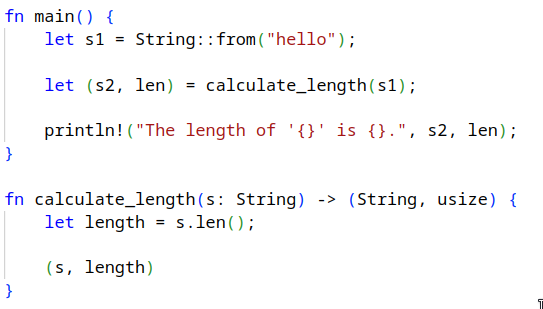
\includegraphics[keepaspectratio, width=12cm]{gambar/print-string-and-length.png}
  \caption{Program untuk mencari panjang dari \emph{string} dalam \emph{rust} \citep{rustbook}}
	\label{gambar:rust-length-string}
\end{figure}

Dalam kode \ref{gambar:rust-length-string} fungsi \emph{calculate\_length} berfungsi untuk menghitung panjang dari string, dalam fungsi tersebut terdapat dua \emph{return value} dikarenakan fungsi tersebut ketika menerima parameter \emph{string} \emph{s1} secara otomatis \emph{ownership} dari variabel tersebut diberikan ke \emph{calculate\_length}. Agar kode \ref{gambar:rust-length-string} dapat mengakses kembali nilai \emph{string} dalam \emph{s1} fungsi \emph{calculate\_length} perlu juga memberikan \emph{return value} berupa \emph{string} tersebut, keterbatasan penggunaan variabel yang berinteraksi dengan parameter suatu fungsi membuat fungsi \emph{calculate\_length} menjadi kompleks. Untuk mengindari kompleksitas tambahan yang diasosiasikan dengan pemindahan \emph{ownership} kepada fungsi lain perlu digunakan \emph{reference} atau \emph{borrowing} \citep{rustbook}. 

\emph{Referece} merupakan sebuah \emph{pointer} yang menunjuk kepada alamat dari data asli tersebut dalam \emph{memory}. Ketika suatu variabel dibuat \emph{reference}-nya, \emph{ownership} dari data tersebut masih terikat dengan variabel asalnya dan \emph{reference} tersebut hanya berisi alamat variabel asal-nya saja \citep{rustbook}. 

\begin{figure}[H]
  \centering
  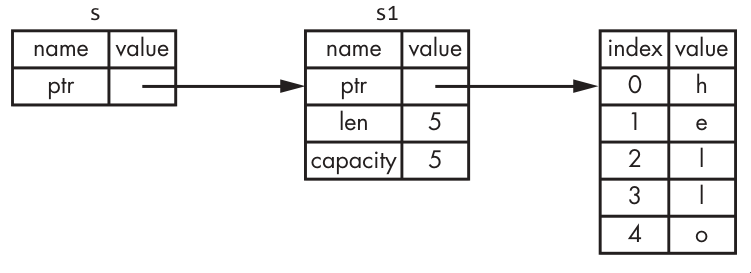
\includegraphics[keepaspectratio, width=12cm]{gambar/reference-memory.png}
  \caption{Representasi penggunaan \emph{referece} dalam \emph{memory} \citep{rustbook}}
  \label{gambar:reference-memory-ilust}
\end{figure}

Dari kode \ref{gambar:reference-memory-ilust} dapat dilihat bahwa variabel \emph{s} yang merupakan \emph{reference} dari \emph{s1}, maka \emph{s} hanya menyimpan data mengenai alamat dari variabel \emph{s1} saja dan sisa dari data disimpan di \emph{s1} \citep{rustbook}.

\begin{figure}[H]
  \centering
  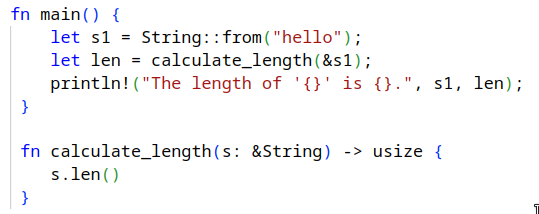
\includegraphics[keepaspectratio, width=12cm]{gambar/reference-rust-code.png}
  \caption{Semantik penggunaan \emph{reference} dalam \emph{rust} \citep{rustbook}}
  \label{gambar:reference-code-rust}
\end{figure}

Kode dalam gambar \ref{gambar:reference-code-rust} merupakan contoh penggunaan \emph{reference} dalam \emph{rust} yang direpresentasikan dalam gambar \ref{gambar:reference-memory-ilust}. Dikarenakan \emph{ownership} dari data tidak berpindah saat \emph{reference} digunakan, maka penggunaaan \emph{reference} dalam parameter fungsi disebut dengan nama \emph{borrowing}. \emph{Borrowing} adalah aksi ketika fungsi meminjam data dari variabel menggunakan \emph{reference} sehingga \emph{ownership} dari data tersebut akan dikembalikan ke variabel yang memiliki \emph{ownership} dari data tersebut. Dapat dilihat dari kode dalam gambar \ref{gambar:reference-memory-ilust} ketika \emph{reference} dari \emph{s1} dimasukkan ke dalam fungsi \emph{calculate\_length}, \emph{ownership} dari data-nya tidak di pindahkan ke variabel \emph{s} tetapi fungsi tetap dapat melakukan operasi terhadap data tersebut dan ketika fungsi \emph{calculate\_length} selesai dijalankan data dari variabel tersebut tidak dihapus.  \citep{rustbook}.

\subsection{Semantik Struktur Data dalam \emph{Rust}}

\emph{Struct} atau \emph{Structure} merupakan tipe data khusus yang dapat mengelompokkan dan menamakan lebih dari satu tipe data yang berkaitan, \emph{struct} digunakan sebagai metode untuk menyimpan struktur data yang lebih kompleks dengan komposisi data yang bervariasi.\citep{rustbook}

\begin{figure}[H]
  \centering
  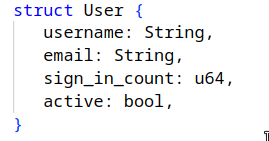
\includegraphics[keepaspectratio, width=7cm]{gambar/struct-declare-rust.png}
  \caption{\emph{Struct} yang mendefinisikan data \emph{user} \citep{rustbook}}
  \label{gambar:struct-definition-rust}
\end{figure}

Kode \ref{gambar:struct-definition-rust} merupakan mekanisme dalam mendefinisikan \emph{struct} dalam \emph{rust}, \emph{struct} itu diberi nama \emph{user} dan berisi data-data seperti \emph{username}, \emph{email}, \emph{sign in count}, dan \emph{active} dengan tipe data yang berbeda-beda. \emph{Struct} hanya mendefinisikan rancangan dari tipe data khusus yang akan dibuat dan selama data ini belum diinisiasi belum ada ruang dalam \emph{memory} dinamis yang dialokasikan \citep{rustbook}.

\begin{figure}[H]
  \centering
  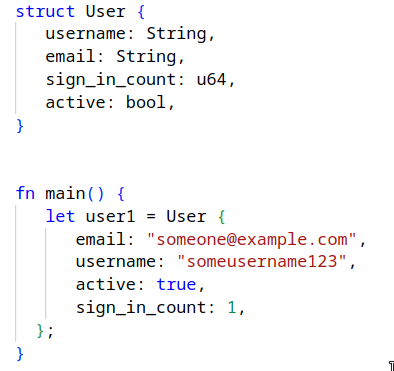
\includegraphics[keepaspectratio, width=9cm]{gambar/rust-object-declaration.png}
  \caption{Deklarasi objek dalam \emph{rust} \citep{rustbook}}
  \label{gambar:object-declaration-rust}
\end{figure}

Untuk menggunakan struktur data yang didefinisikan dalam \emph{struct} diperlukan untuk membuat objek atau \emph{instance} dari \emph{struct} tersebut, kode dalam gambar \ref{gambar:object-declaration-rust} variabel \emph{user1} merupakan objek atau \emph{instance} yang dibuat berdasarkan \emph{struct} \emph{user}. Dalam pembuatan objek \emph{user1}, data-data atau \emph{fields} yang menyusun objek tersebut diisi dengan nilai-nilai tertentu seperti data \emph{username} yang diisi dengan nilai \emph{someusername123}. Objek yang telah dibuat berdasarkan desain dari \emph{struct} dapat digunakan sebagai tempat untuk menyimpan data yang kompleks, dan data-data tersebut dapat diakses ataupun di modifikasi saat jalannya program \citep{rustbook}.

\begin{figure}[H]
  \centering
  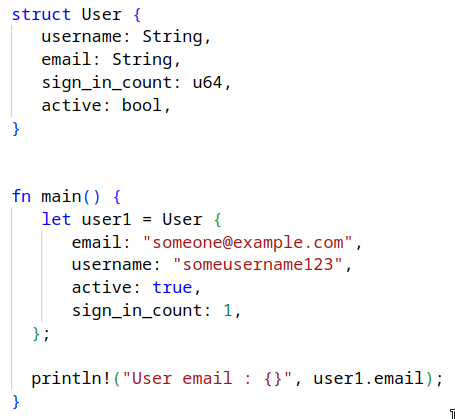
\includegraphics[keepaspectratio, width=9cm]{gambar/rust-accessing-attributes.png}
  \caption{Mengakses atribut kelas di \emph{Rust} \citep{rustbook}}
  \label{gambar:attributes-accesing-rust}
\end{figure}

\emph{Attributes} atau data yang disimpan di dalam \emph{struct} dapat diakses dengan memanggil objek tersebut seperti yang ditunjukan pada kode dalam gambar \ref{gambar:attributes-accesing-rust}. Dengan memanggil nama objek \emph{user1} yang diinisasi menggunakan sesuai dengan \emph{struct} \emph{User} dan mengakses \emph{attributes} email, data dari \emph{attributes} email dapat diakses dan diubah secara langsung \citep{rustbook}.

Selain menggunakan \emph{struct}, \emph{rust} juga menyediakan cara lain dalam menyimpan data kompleks yaitu \emph{enum}. \emph{Enum} atau \emph{enumerates} merupakan struktur data untuk meyimpan data yang merupakan kemungkinan dari pilihan kumpulan data, perbedaan yang paling mencolok antara \emph{struct} dan \emph{enum} adalah \emph{struct} menyimpan data yang terkait dan dapat diibaratkan dengan kata dan sedangkan \emph{enum} menyimpan data terkait yang merupakan pilihan yang dapat diibaratkan dengan kata atau.\citep{rustbook}

\begin{figure}[H]
  \centering
  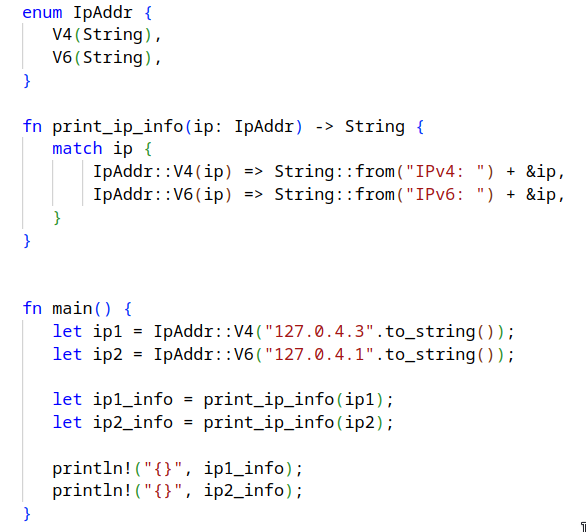
\includegraphics[keepaspectratio, width=12cm]{gambar/rust-enum-operations.png}
  \caption{Operasi yang memanfaatkan \emph{enum} pada \emph{rust} \citep{rustbook}}
  \label{gambar:enum-operations-rust}
\end{figure}

Dalam kode \ref{gambar:enum-operations-rust}, pendeklarasian \emph{enum} \emph{IpAddr} dilakukan pertama kali. Sama seperti \emph{struct}, \emph{enum} \emph{IpAddr} hanyalah struktur data rancangan dan data baru di deklarasikan di fungsi \emph{main} saat pembuatan variabel \emph{ip1}. Perbedaan \emph{enum} dengan \emph{struct} dapat dilihat dari isi \emph{enum} yang dideklarasikan, dimana saat deklarasi \emph{enum} variabel yang dibuat harus memilih diantara pilihan attribut yang ada \citep{rustbook}.

\begin{figure}[H]
  \centering
  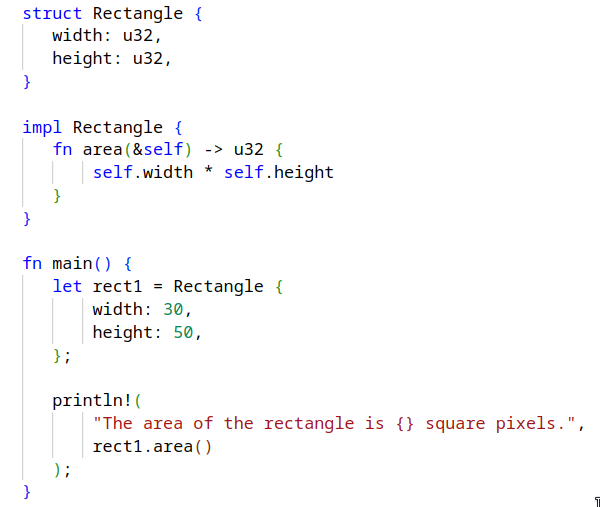
\includegraphics[keepaspectratio, width=12cm]{gambar/rust-struct-method.png}
  \caption{\emph{Method} dalam \emph{rust} \citep{rustbook}}
  \label{gambar:method-struct-rust}
\end{figure}

Metode yang disarankan untuk operasi yang mengubah nilai dari data yang disimpan dalam \emph{struct} dan \emph{enum} adalah menggunakan \emph{method}. \emph{Method} pada dasarnya serupa dengan \emph{function}, perbedaan-nya adalah \emph{method} merupakan \emph{function} yang di-definisikan dalam konteks \emph{struct} atau \emph{enum}. \emph{Method} dapat dengan bebas memodifikasi semua data yang disimpan di dalam \emph{struct} atau \emph{enum}. Seperti kode dalam gambar \ref{gambar:method-struct-rust}, parameter pertama dari \emph{method} adalah \emph{self} yang merepresentasikan objek dari \emph{struct} atau \emph{enum} yang terkait \citep{rustbook}.


%!TEX root = ./template-skripsi.tex
%-------------------------------------------------------------------------------
%                            BAB III
%               			PEMBAHASAN
%-------------------------------------------------------------------------------

\chapter{DESAIN MODEL}

\section{Tahapan Penelitian}

Diagram \emph{flowchart} dalam gambar \ref{gambar:diagram_experiment} menggambarkan proses modifikasi dari arsitektur \emph{search engine} orisinil menjadi arsitektur \emph{search engine} yang ter-improvisasi.

\begin{figure}[H]
	\centering
	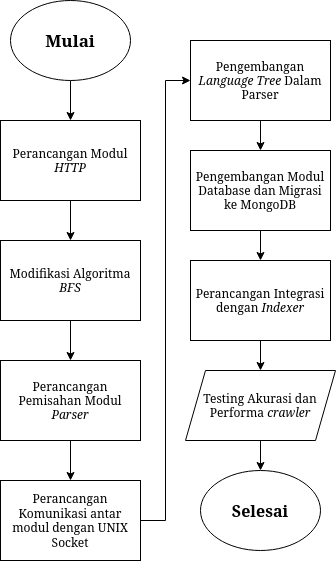
\includegraphics[keepaspectratio, width=7cm]{gambar/experiment-diagram.png}
	\caption{Diagram Tahapan Penelitian}
	\label{gambar:diagram_experiment}
\end{figure}

Proses modifikasi dimulai dengan melakukan konversi modul searah dengan jalannya data ketika proses \emph{crawling}, ini dilakukan untuk mempermudah \emph{testing} terhadap jalannya \emph{crawler}. Modul pertama yang perlu dikonversi adalah modul pengunduhan data atau modul \emph{http}, selanjutnya merancang bagaimana modul \emph{http} dapat berjalan secara \emph{asyncronously} menggunakan \emph{threads}. Modul kedua yang perlu dikonversi adalah \emph{parser}, dalam melakukan konversi \emph{parser} perlu dilakukan pemisahan \emph{parser} dengan modul \emph{http} maka pengkonversian modul \emph{parser} juga dilakukan bersamaan dengan perancangan pemisahan modul tersebut dan metode komunikasi apa yang perlu dilakukan. Modul \emph{database} dikembangkan setelah modul \emph{parser} selesai di-konversikan, karena sumber data-nya berasal dari \emph{parser}, dan selanjutnya juga perlu direncanakan bagaimana \emph{crawler} dapat terintegrasi dengan \emph{indexer}. 

Selain konversi modul, perlu juga dilakukan perancangan algoritma \emph{breadth-first search} yang dimodifikasi untuk meningkatkan akurasi \emph{crawling} per \emph{thread}, algoritma ini akan diintergasikan kedalam modul \emph{http} karena proses \emph{breadth-first search} berkaitan erat dengan proses pengunduhan dan penjelajahan \emph{url}. Hal lain yang perlu diperhatikan adalah ketika proses konversi selesai perlu dilakukan \emph{testing} dan \emph{profiling} untuk memastikan \emph{crawler} termodifikasi ini berjalan lebih cepat daripada \emph{crawler} orisinil.


\section{Modifikasi Arsitektur \emph{Crawler}}

\begin{figure}[H]
	\centering
	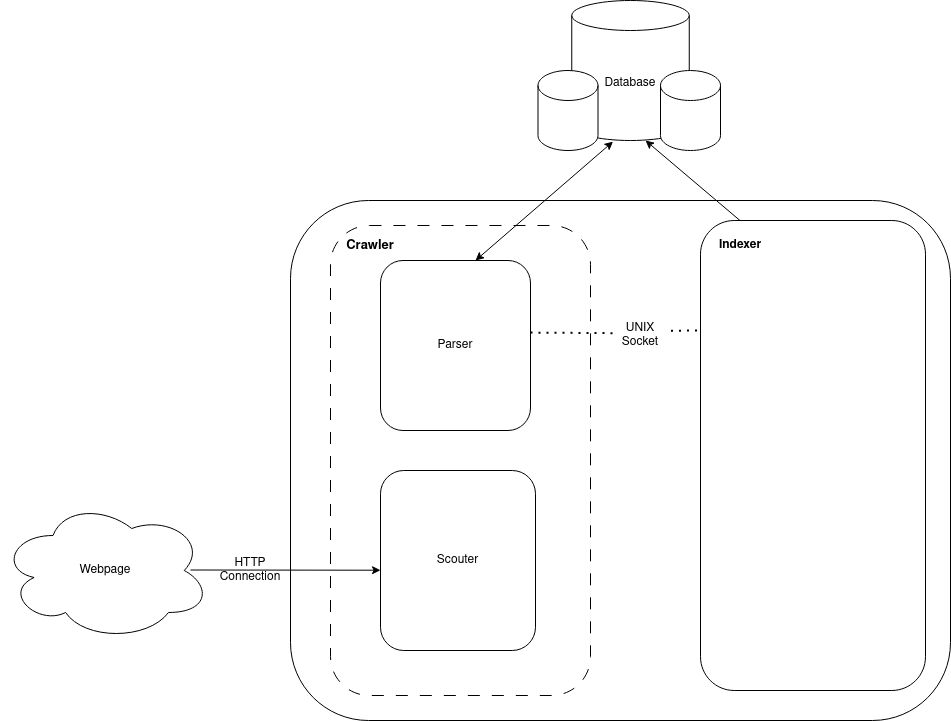
\includegraphics[keepaspectratio, width=15cm]{gambar/crawler-multiprocess-architecture.png}
	\caption{Diagram Arsitektur Crawler Termodifikasi}
	\label{gambar:arsitektur_diagram}
\end{figure}

Dari arsitektur \emph{crawler} yang sudah ada saat ini terdapat beberapa modifikasi yang perlu dilakukan untuk memperbaiki performa proses \emph{crawling}.

\begin{itemize}
  \item Arsitektur ini akan dibagi menjadi 2 \emph{service} yaitu, \emph{crawler} dan \emph{indexer}.
  \item \emph{Service} \emph{Crawler} akan dibagi menjadi dua \emph{process}, \emph{Scouter} dan \emph{Parser}. \emph{Scouter} bertugas sebagai pengunduh halaman \emph{website} dan \emph{parser} bertugas sebagai pembagun \emph{language tree} dan melakukan \emph{input} kedalam \emph{database}.
  \item Jalannya \emph{crawler} dan \emph{indexer} akan secara bersamaan dan otomatis. Untuk mengontrol jalannya \emph{indexer} agar konsistensi data dapat terjaga, 
\end{itemize}

\section{Algoritma modifikasi \emph{Breadth-first search} dengan \emph{domain constraint}}

Untuk menyeragamkan jumlah halaman \emph{web} yang diakses oleh tiap \emph{thread}, algoritma \emph{breadth-frst search} yang digunakan untuk mengunjungi tiap-tiap halaman perlu dimodifikasi. Modifikasi yang dilakukan adalah dengan menugaskan jalannya \emph{crawler} di tiap \emph{thread} sebuah domain \emph{url} tertentu, dan membatasi \emph{url} yang dapat diakses oleh \emph{thread} tersebut sesuai dengan \emph{url} yang telah ditugaskan. Setiap \emph{thread} akan mengambil dan menyimpan \emph{url} di dalam \emph{queue} global, \emph{queue} ini merupakan \emph{multi-lock queue} dengan format yang lebih kompleks dari \emph{queue} normal, ini dilakukan agar tidak terjadi \emph{race condition} antar \emph{thread} ketika mengambil ataupun menyimpan data kedalam \emph{queue} tersebut. Gambar \ref{gambar:diagram_modified_bfs} merupakan ilustrasi dari jalannya algoritma \emph{breadth-first search} termodifikasi.

\begin{figure}[H]
	\centering
	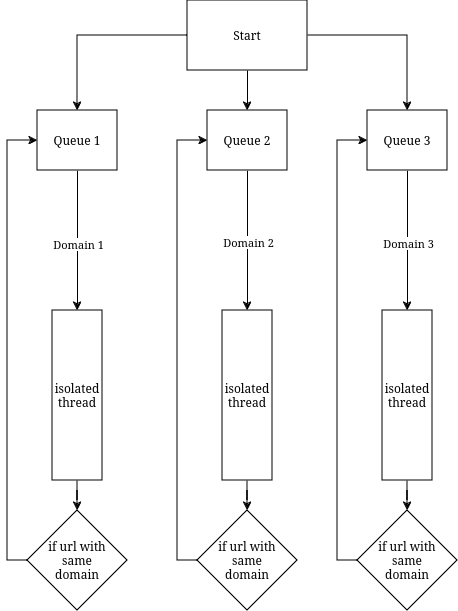
\includegraphics[keepaspectratio, width=8cm]{gambar/modified-bfs-diagram.png}
  \caption{Diagram cara kerja algoritma \emph{breadth-first search} termodifikasi}
	\label{gambar:diagram_modified_bfs}
\end{figure}

\begin{algorithm}[H]
  \caption{Algoritma \emph{breadt first search} termodifikasi}
	\label{Typical_crawling_model}
  \algblockdefx[Name]{ThreadStart}{ThreadEnd}%
    [1][Unknown]{$\textbf{Thread}(#1).Start$}%
    {$\textbf{Thread}.Stop()$}
	\begin{algorithmic}[1]
    \Require{$ P \gets [p_{1}, p_{2}, ..., p_{n}]$ }
    \Function{$BreadthFirstSearch$}{$P$}
      \State $Q \gets {P}$ \Comment{Global multi-lock queue}
      \State $V \gets [..]$ \Comment{visited URLs.} 
      \For{$p_{n} \in Q$}
        \State Async $ScrapPage(p_n)$ \Comment{dijalankan dalam \emph{thread}}
      \EndFor
    \EndFunction
    \Statex
    \Function{$ScrapPage$}{$p_n$}
		    \While{$Q\not=\emptyset$}
		      \State Dequeue $p \in Q$
          \If{$p_{n} (base\_url) = p_{n-1} (base\_url)$}
            \State $ p\_html \gets Fetch(p)$
            \State $Append(V, p)$
            \State $ p\_info \gets ParsePage(p\_html)$
            \For{$links \in p\_info.links$}
              \If{$links \notin V$}
                \State $Append(Q, links)$
              \EndIf
            \EndFor
          \EndIf
		    \EndWhile
    \EndFunction
	\end{algorithmic}
\end{algorithm}

Dalam kode diatas modifikasi dilakukan pada bagian diamana sebelum \emph{links} ditambahkan kedalam \emph{queue}, dilakukan pengecekan terlebih dahulu untuk verifikasi \emph{domain} dari \emph{link} yang akan dimasukkan.

\section{Konversi modul \emph{http}}

Proses pertama yang dilakukan oleh crawler adalah mengunduh halaman \emph{website} atau yang dapat \emph{fetching} , proses ini dilakukan melalui \emph{http get} \emph{request} terhadap \emph{url} dari halaman \emph{website} yang ingin di-unduh. Informasi yang di dapat dari proses \emph{fetching} adalah \emph{url} halaman, konten \emph{html} dari halaman tersebut, dan durasi proses \emph{fetch}. Objek \emph{FetchPage} digunakan untuk menyimpan data-data tersebut.

\begin{figure}[H]
	\centering
	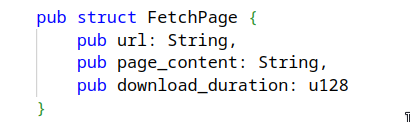
\includegraphics[keepaspectratio, width=10cm]{gambar/http-request-rust-struct.png}
  \caption{Struktur Data yang digunakan untuk operasi \emph{fetching} \emph{http}}
	\label{gambar:http_struct_rust}
\end{figure}

\emph{FetchPage} juga digunakan sebagai \emph{blueprint} dalam definisi modul dan metode \emph{fetching}. Fungsi untuk melakukan \emph{fetching} akan dibuat sebagai \emph{method} dari objek \emph{FetchPage}. \emph{Methdo} \emph{Fetch} merupakan fungsi untuk melakukan pengunduhan, sedangkan \emph{New} adalah fungsi untuk membuat objek \emph{FetchPage} baru yang hanya berisi \emph{url} saja. Untuk mendukung jalannya fungsi \emph{Fetch} secara \emph{asyncronously} dalam modul ini menggunakan dua \emph{library}, yaitu \emph{tokio} dan \emph{reqwest}.

\begin{table}[H]
  \caption{\emph{Library} yang digunakan dalam modul \emph{HTTP}}
  \begin{center}
    \begin{tabular}{ |p{1cm}|p{3cm}|p{7cm}| } \hline
      \textbf{no}.& \textbf{\emph{library}}& \textbf{deskripsi} \\ \hline
      1& \emph{tokio}& Library untuk menjalankan dan mengatur jalannya kode secara bersamaan \\ \hline
      2& \emph{reqwest}& Library untuk membuat dan menjalankan \emph{HTTP} \emph{GET} \emph{request} \\ \hline
    \end{tabular}
  \end{center}
\end{table}

\begin{figure}[H]
	\centering
	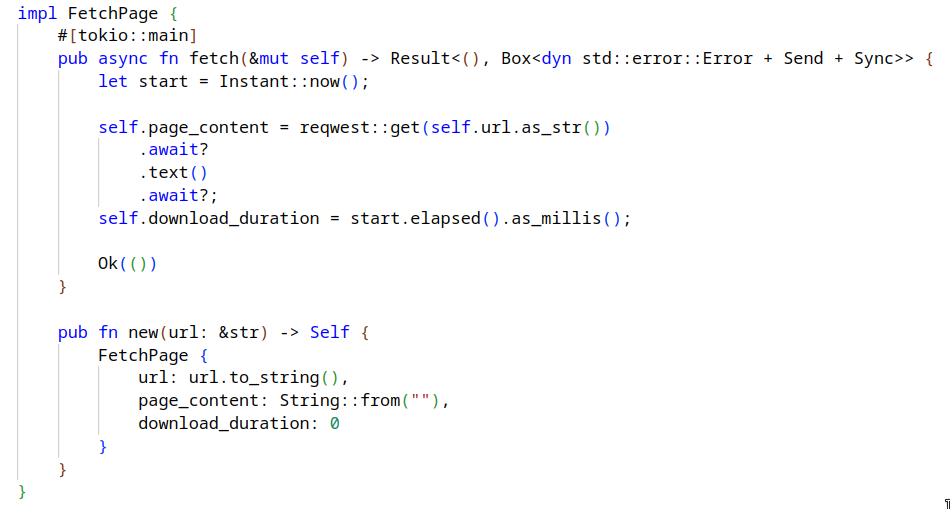
\includegraphics[keepaspectratio, width=15cm]{gambar/http-request-rust-method.png}
  \caption{Fungsi yang digunakan untuk melakuan operasi \emph{fetching} \emph{http}}
	\label{gambar:http_method_rust}
\end{figure}

\section{Perancangan Pemisahan dan Sinkronisasi Proses Module \emph{parser}}

Teks \emph{html} dari modul fetch selanjutnya akan di pindahkan ke modul \emph{parser} untuk diambil informasi-nya. Karena modul \emph{parser} terletak di \emph{process} \emph{rust} yang berbeda, terdapat dua bagian kode yang mengontrol proses ini yaitu,

\begin{enumerate}
  \item Modul sinkronsasi
  \item Modul \emph{parser}
\end{enumerate}

\subsection{Sinkronisasi Menggunakan \emph{UNIX Socket}}

Pengiriman dan sinkronisasi data dalam modul \emph{scouter} dengan dengan modul \emph{parser} dilakukan dengan menggunakan \emph{UNIX Socket}. Sinkronisasi data diatur dengan menggunakan data mentah dari halaman \emph{web} yang sudah diunduh oleh \emph{scouter}, mekanisme dari komunikasi \emph{UNIX Socket} adalah program akan menngirimkan teks \emph{HTML} yang diformat sebagai \emph{memory buffer} yang berbentuk \emph{slice of bytes}.

\begin{figure}[H]
	\centering
	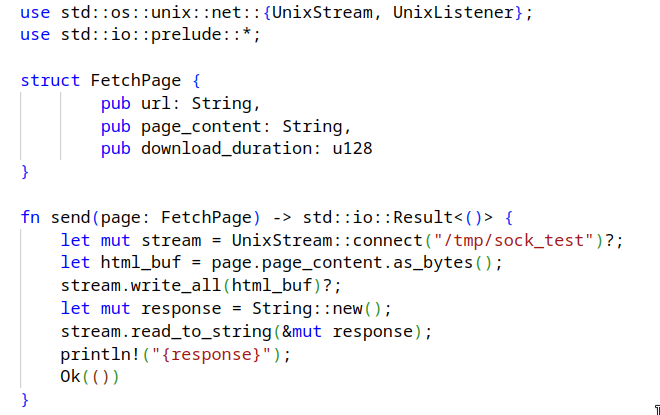
\includegraphics[keepaspectratio, width=10cm]{gambar/unix-sock-send-rs.png}
  \caption{Fungsi yang digunakan untuk melakukan operasi pengiriman teks \emph{html} mengguanak \emph{UNIX Socket}}
	\label{gambar:unix-socket-send}
\end{figure}

\emph{Messages} yang dikirim akan di-konsumsi oleh \emph{receiver} di \emph{process} lain, \emph{messages} ini yang akan di ubah kembali menjadi string dan diproses menuju proses \emph{parsing}. Keseluruhan proses ini perlu menggunakan file sementara dalam sistem \emph{UNIX} sebagai \emph{placeholder} untuk \emph{message}. Proses ini hanya perlu menggunakan \emph{stdlib} dari \emph{rust} untuk menangani pengiriman dan penerimaan \emph{message}.

\begin{figure}[H]
	\centering
	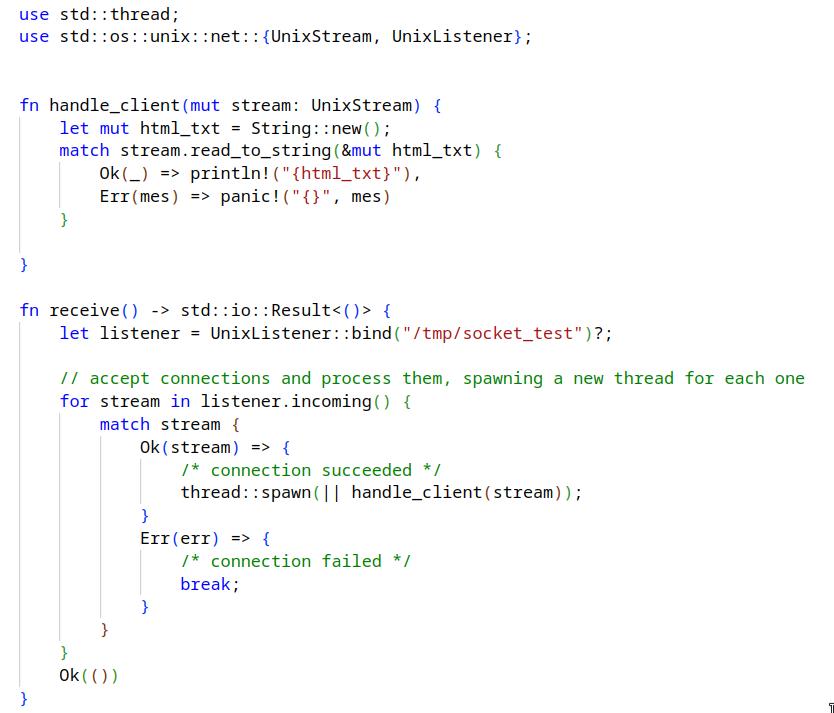
\includegraphics[keepaspectratio, width=12cm]{gambar/unix-sock-receive-rs.png}
  \caption{Fungsi yang digunakan untuk melakukan operasi penerimaan teks \emph{html} mengguanak \emph{UNIX Socket}}
	\label{gambar:unix-socket-receive}
\end{figure}


\subsection{Modul Proses \emph{Parser}}

Data mentah teks \emph{html} yang masuk ke dalam modul \emph{parser} selanjutnya akan di-\emph{parse} untuk mendapatkan informasi-informasi penting dari halaman \emph{web} tersebut. Proses \emph{parsing} ini pada dasarnya hanya membangun struktur \emph{language tree} dari halaman \emph{web} sehingga informasi yang berada di dalam \emph{html tag} lebih mudah untuk di dapatkan. Objek \emph{PageInformation} berfungsi sebagai tempat untuk menyimpan data-data penting per halaman \emph{web}.

\begin{figure}[H]
	\centering
	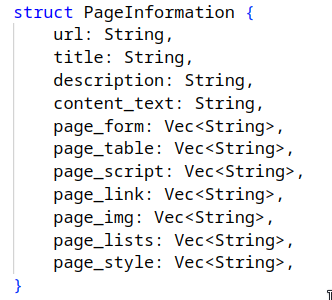
\includegraphics[keepaspectratio, width=7cm]{gambar/parse-object-rs.png}
  \caption{Objek \emph{PageInformation} yang menyimpan data-data hasil proses \emph{parsing} halaman \emph{web}}
	\label{gambar:parse_object}
\end{figure}

Fungsi \emph{parsing} yang akan dipanggil akan dibuat sebagai \emph{method} dari objek \emph{PageInformation}, \emph{parse\_page} sebagai fungsi yang melakukan operasi \emph{parsing} tersebut hanya membangun \emph{language tree} satu kali saat pembuatan variabel \emph{document}. Bagian-bagian \emph{tag HTML} di cari dan di ambil mengguanakn selector yang disesuaikan dengan pola kemunculannya. Informasi tersebut di kumpulkan, beberapa di \emph{input} kedalam bentuk data \emph{vector} dan di masukkan kedalam objek \emph{PageInformation}. Proses ini menggunakan \emph{third-party library} yang bernama \emph{scraper}.

\begin{figure}[H]
	\centering
	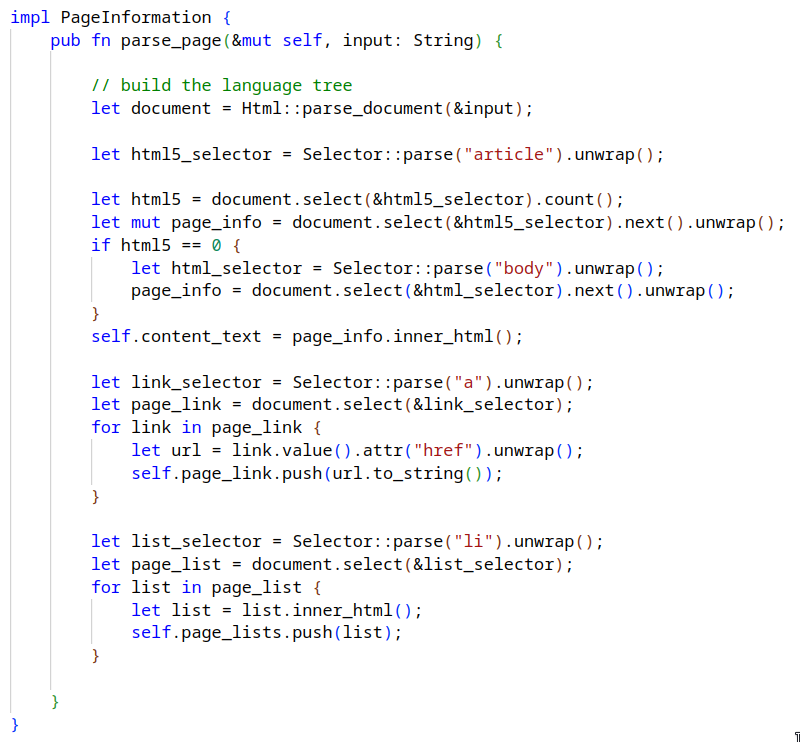
\includegraphics[keepaspectratio, width=15cm]{gambar/parse-method-rs.png}
  \caption{Method \emph{parse\_page} yang mengambil dan menyimpan data-data dari halaman \emph{web} kedalam objek \emph{PageInformation}}
	\label{gambar:parse_method}
\end{figure}

\vspace{0.5cm}

\section{Perancangan konversi modul \emph{database}}

Sebagai cara untuk meningkatkan performa dari \emph{crawler}, penyimpanan data akan diubah dari yang sebelumnya menggunakan \emph{MySql} menjadi menggunakan \emph{MonggoDB}. Struktur dari data yang akan disimpan akan sama tetapi dengan modifikasi terbatas agar dapat tersimpan dengan baik. Pernyimpanan data akan diatur menggunakan Objek untuk mempertahankan konsistensi format data dalam \emph{database}.

\begin{figure}[H]
	\centering
	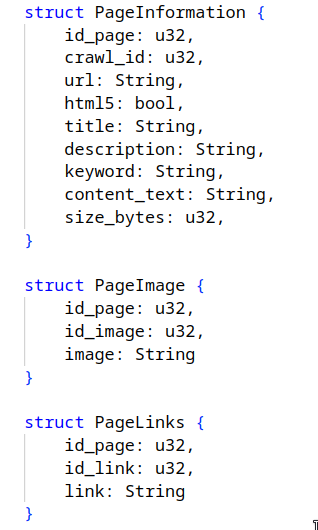
\includegraphics[keepaspectratio, width=5cm]{gambar/rust-db-struct.png}
  \caption{Contoh objek skema penyimpanan data kedalam \emph{database} dalam \emph{rust}}
	\label{gambar:unix_sock_indexer}
\end{figure}

Modifikasi lain yang dapat dilakukan untuk mempercepat proses penyimpanan data adalah dengan menggunakan bulk insert. Berbeda dengan \emph{crawler} sebelumnya yang melakukan penyimpanan pada tiap data satu persatu dengan menggunakan\emph{looping}, \emph{crawler} termodifikasi akan menggunakan mekanisme \emph{bulk insert} yang menjalankan proses penyimpanan hanya sekali.

\section{Perancangan modul sinkronisasi dengan proses \emph{indexing}}

Sinkronisasi dengan proses \emph{indexing} dilakukan dengan memanfaatkan \emph{UNIX Socket}. Sinkronisasi data akan diatur dengan data terformat yang berisi \emph{id\_page} dan \emph{url} dari halaman \emph{web} yang telah disimpan didalam \emph{database}, data ini akan dikirimkan oleh \emph{crawler} setelah menyimpan data dan diterima oleh \emph{indexer}. Dikarenakan \emph{UNIX Socket} merupakan metode komunikasi yang \emph{platform independent} maka tidak perlu ada pengkonversian modul \emph{indexer} kedalam bahasa pemograman \emph{rust}. 

\begin{figure}[H]
	\centering
	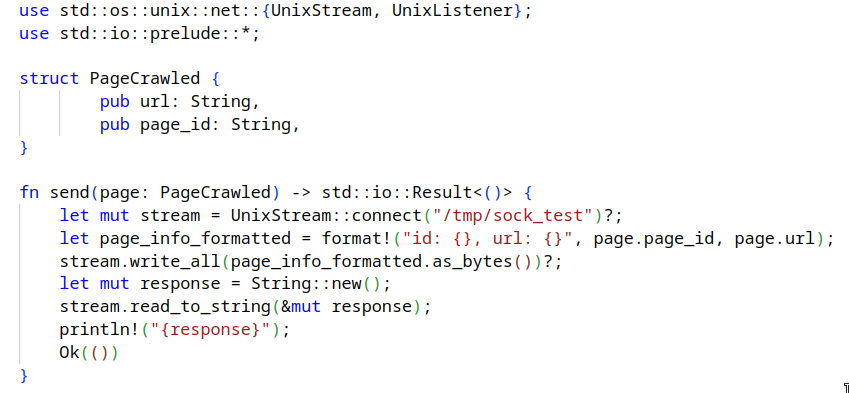
\includegraphics[keepaspectratio, width=15cm]{gambar/unix-sock-indexing.png}
  \caption{Objek dan \emph{method} dalam modul \emph{crawler} sebagai pengirim data menuju \emph{indexer}}
	\label{gambar:unix_sock_indexer}
\end{figure}

\section{Alat dan Bahan Penelitian}

Alat penunjang yang digunakan dalam pengembangan modifikasi \emph{crawler} ini dituliskan dibawah ini:
\begin{itemize}
  \item Laptop dengan konfigurasi Ryzen 4500u 6 core 6 threads, 20GB RAM
  \item Sistem operasi \emph{linux}
  \item \emph{Neovim} sebagai \emph{code editor}
  \item \emph{Docker} untuk mengelola \emph{database} dan \emph{service}
  \item \emph{Rust Programming Language} versi 1.73.0
\end{itemize}

\section{Desain Eksperimen}

\subsection{Modifikasi dan Pengkonversian modul-modul \emph{Crawler}}

Konversi dilakukan sesuai dengan urutan data dalam proses \emph{crawler} orisinil, setiap sub-modul dan proses akan dibuat sebagai modul dengan objek dan \emph{method} untuk memudahkan perpindahan data dari satu sub-modul ke sub-modul yang lain. Konversi dimulai dari sub-modul \emph{http}, sub-modul ini menggunakan \emph{library} \emph{Tokio} dan \emph{reqwest} untuk menjalankan pengunduhan halaman \emph{web}. Data dari sub-modul \emph{http} akan di proses oleh \emph{parser}, sub-modul \emph{parser} dipisah dari sub-modul \emph{http} dalam \emph{process} yang berbeda dan komunikasi antar \emph{process} menggunakan \emph{UNIX Socket}. \emph{Parser} ini digunakan untuk membangun \emph{language tree} dan objeck dalam sub-modul ini berisi data-data yang perlu di ambil dari \emph{html} halaman \emph{web}. Data yang dikumpulkan oleh \emph{parser} akan disimpan dalam database \emph{mongodb}, sebagai \emph{blueprint} dari struktur data dalam \emph{database} tidak akan dirumah untuk menjaga konsistensi data. Setelah data disimpan, modul ini akan mengirim pesan kepada \emph{indexer} untuk memulai proses \emph{indexing}. Gambar \ref{gambar:old_crawler_diagram} merupakan gambaran dari cara kerja \emph{crawler} lama sedangkan gambar \ref{gambar:new_crawler_diagram} merupakan diagram cara kerja \emph{crawler} baru.

\begin{figure}[H]
	\centering
	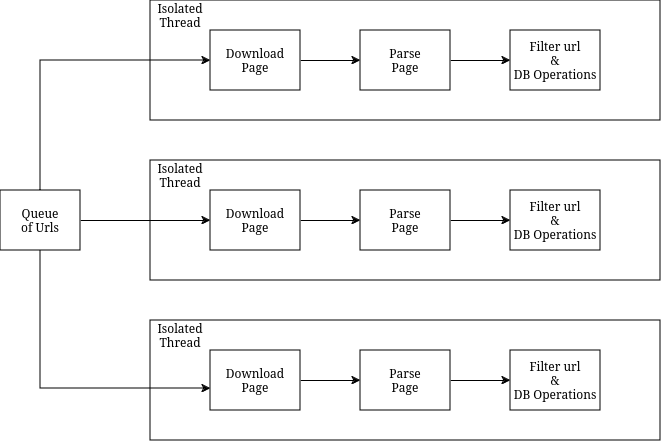
\includegraphics[keepaspectratio, width=10cm]{gambar/old-crawler-multithread-diagram.png}
  \caption{Ilustrasi cara kerja \emph{crawler} lama}
	\label{gambar:old_crawler_diagram}
\end{figure}

\begin{figure}[H]
	\centering
	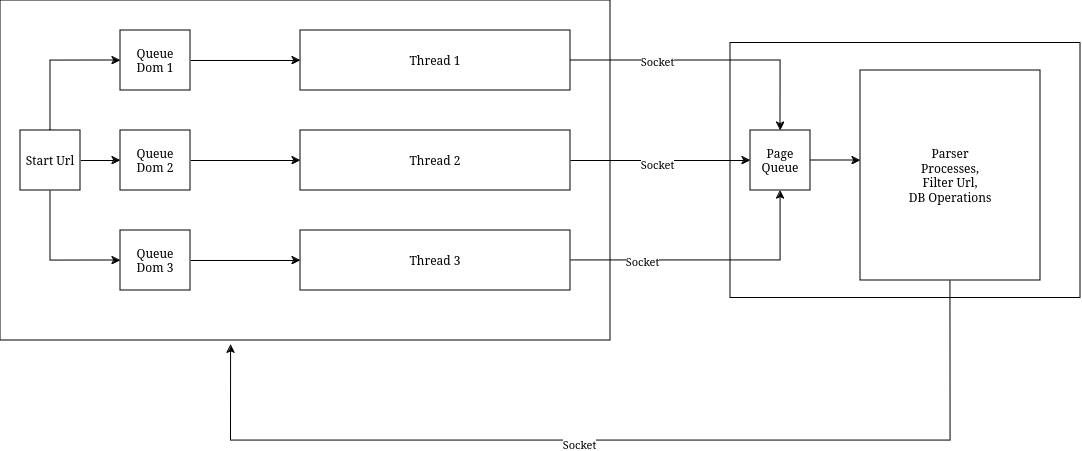
\includegraphics[keepaspectratio, width=10cm]{gambar/new-crawler-multithread-diagram.png}
  \caption{Ilustrasi cara kerja \emph{crawler} baru}
	\label{gambar:new_crawler_diagram}
\end{figure}

\subsection{\emph{Testing}}

Setelah semua modul berhasi di konversikan, perlu dilakukan testing untuk menilai performa \emph{crawler} termodifikas terhadap \emph{crawler} orisinil. Terdapat beberapa poin dari \emph{crawler} yang perlu di-test untuk menilai peningkatan performa yaitu,

\begin{enumerate}
  \item Jumlah halaman yang berhasil dikunjungi selama proses \emph{crawling}
  \item Persentase halaman per-domain yang berhasil dikunjungi relatif terhadap total halaman yang dikunjungi oleh \emph{crawler}
  \item Waktu yang dihabiskan dalam pengambilan informasi dari satu halaman
  \item Konsistensi data yang terkumpul
\end{enumerate}

%!TEX root = ./template-skripsi.tex
%-------------------------------------------------------------------------------
%                             BAB IV
%                   KESIMPULAN DAN SARAN
%-------------------------------------------------------------------------------

\chapter{HASIL DAN PEMBAHASAN}

\section{Implementasi}

\begin{figure}[H]
  \centering
  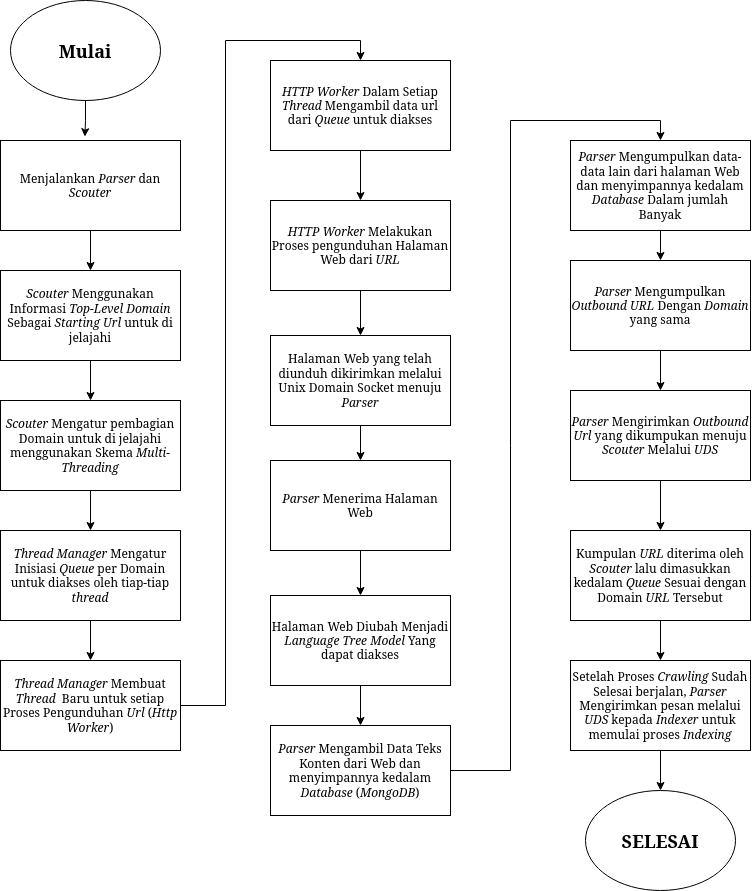
\includegraphics[keepaspectratio, width=12cm]{gambar/flowchart-penelitian.png}
  \caption{Diagram perencanaan penelitian}
  \label{gambar:flowchart_experiment}
\end{figure}

Diagram \ref{gambar:flowchart_experiment} merupakan alur tahapan penelitian yang berhasil diselesaikan, \emph{flowchart} ini merupakan penyempurnaan dari diagram perencanaan penelitan di bab 3. Secara umum terdapat dua aplikasi atau \emph{services} yang dijalankan dalam penelitian ini yaitu \emph{scouter} dan \emph{crawler} dimana \emph{scouter} bertugas sebagai penjelajah \emph{url}, pengelola akses \emph{queue} per domain, pengunduh halaman web, dan akses utama serta \emph{entry point} dari arah jalan data. \emph{Parser} sebagai pengakses \emph{HTML} dari tiap-tiap halaman web, pengambil data, dan melakukan manajemen penyimpanan data kedalam \emph{database}. Proses yang dijalankan oleh kedua \emph{services} ini berjalan secara terus menerus hingga batas waktu yang telah di tentukan dalam \emph{environment variables}.

\begin{figure}[H]
  \centering
  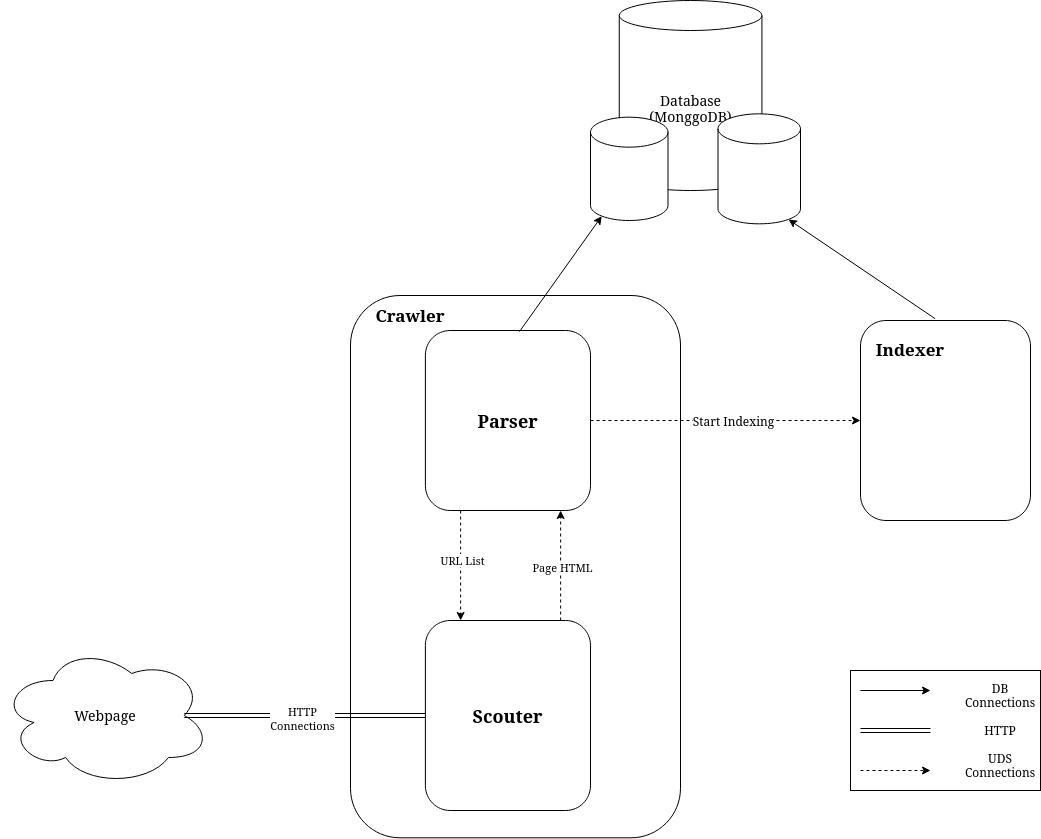
\includegraphics[keepaspectratio, width=12cm]{gambar/high-level-arch.png}
  \caption{Diagram \emph{high-level} Arsitektur Crawler}
  \label{gambar:high_level_arch}
\end{figure}

Diagram \ref{gambar:high_level_arch} merupakan gambaran umum dari arsitektur \emph{web crawler}, terdapat beberapa perbaikan dari diagram bab 3 salah satunya adalah jalur \emph{uds} kedua dari \emph{parser} menuju \emph{scouter} yang membawa \emph{outbound url} dan \emph{message} menuju \emph{indexer} yang hanya berisi \emph{start indexing}. \emph{Scouter} dan \emph{Parser} merupakan dua aplikasi atau \emph{service} bebeda yang dijalankan secara bersamaan. Untuk manajemen dua \emph{services}, menggunakan fitur \emph{workspaces} dari \emph{rust} yang memungkinkan untuk melakukan manajemen dua \emph{source code} dalam satu konteks project.

\begin{figure}[H]
  \centering
  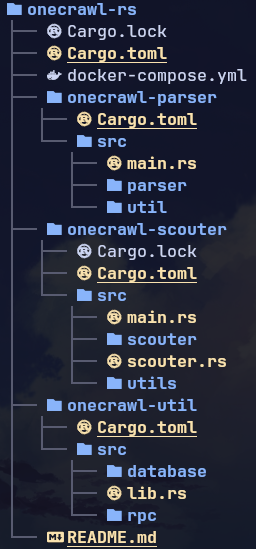
\includegraphics[keepaspectratio, width=5cm]{gambar/project_workspaces.png}
  \caption{Arsitektur penempatan \emph{file} \emph{crawler} seluruh \emph{workspaces}}
  \label{gambar:project_workspaces_arch}
\end{figure}

Gambar \ref{gambar:project_workspaces_arch} merupakan struktur arsitektur keseluruhan \emph{workspaces} dari \emph{web crawler}. Dari gambar \ref{gambar:project_workspaces_arch} dapat dilihat terdapat tiga bagian \emph{workspaces} yaitu \emph{onecrawl-scouter} sebagai \emph{scouter}, \emph{onecrawl-parser} sebagai \emph{parser}, dan \emph{onecrawl-util} sebagai \emph{custom library} yang digunakan oleh kedua \emph{services} tersebut.

\begin{figure}[H]
  \centering
  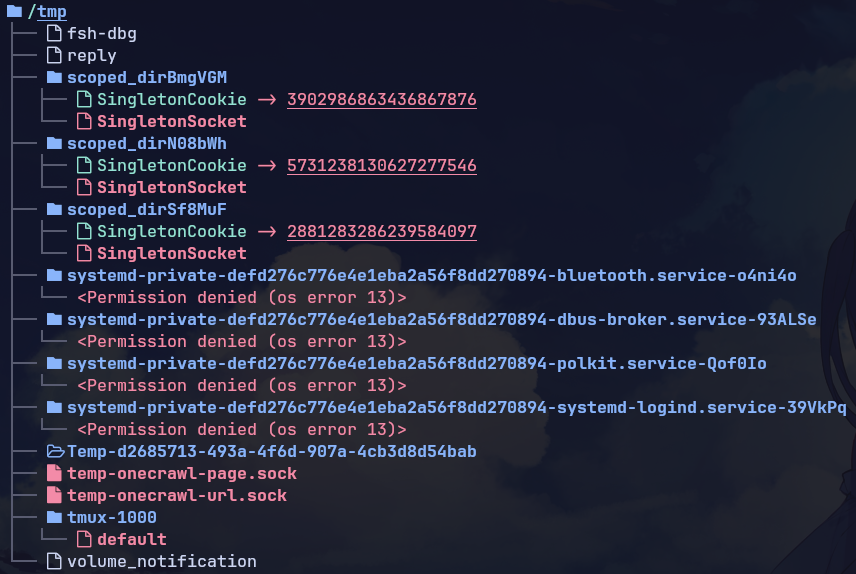
\includegraphics[keepaspectratio, width=10cm]{gambar/uds_pipe_file.png}
  \caption{Dua \emph{file} yang merupakan jalur \emph{Unix Domain Socket} dalam \emph{crawler}}
  \label{gambar:uds_pipe_file}
\end{figure}

Sebagai Jalur komunikasi antar \emph{services}, \emph{Unix Domain Socket} atau \emph{UDS} perlu sebuah file dalam direktori \emph{file} \emph{/tmp} sebagai jalur atau \emph{pipeline} dari pesan-pesan yang dikirimkan. Dalam gambar \ref{gambar:uds_pipe_file} terdapat dua file, \emph{temp-onecrawl-page.sock} sebagai \emph{placeholder} jalur komunikasi dari \emph{scouter} menuju \emph{parser} dan \emph{temp-onecrawl-url.sock} sebagai \emph{placeholder} jalur komunikasi dari \emph{parser} menuju \emph{scouter}.

\subsection{Implementasi algoritma \emph{Breadth-first Search} Modifikasi}

Implementasi algoritma \emph{breadth-first search} termodifikasi dilakukan di kedua \emph{services}, dikarenakan \emph{control flow} untuk akses halaman web berada di \emph{scouter} dan mekanisme pengumpul \emph{url} berada di \emph{parser}. Algoritma \emph{breadth-first search} termodifikasi terdiri dari dua bagian, bagian pengalokasian \emph{thread} terisolasi untuk setiap akses domain dan bagian \emph{filtering} dari \emph{url} yang dikumpulkan agar hanya sesuai dengan \emph{domain} dari halaman web tersebut.

Pembagian tiap domain pertama dilakukan saat \emph{crawler} mulai berjalan pertama kali setelah mengambil \emph{origin url} dari \emph{environment variable}. Dikarenakan setiap \emph{origin url} memiliki domain yang berbeda, tiap \emph{origin url} ini di-\emph{assign} ke \emph{thread} terisolasi masing-masing, yang dimana tiap \emph{thread} tersebut memilki \emph{queue}, \emph{thread id}, dan \emph{domain id} masing-masing sebagai \emph{identifier}.

\begin{figure}[H]
  \centering
  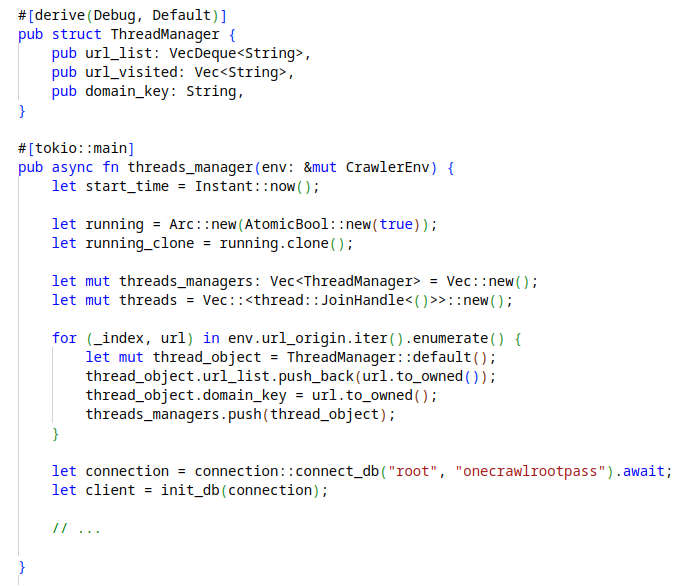
\includegraphics[keepaspectratio, width=10cm]{gambar/code-thread-manager-init.png}
  \caption{Fungsi inisiasi \emph{thread manager} sebagai aktor pengalokasi \emph{thread} untuk masing-masing domain}
  \label{gambar:thread-manager-start-bfs}
\end{figure}

Saat proses \emph{parsing} pengumpulan \emph{url} di \emph{parser} dan sebelum \emph{url list} ini dikirimkan melalui \emph{unix socket}, terlebih dahulu di-\emph{filter} \emph{url} mana yang akan dikirim. Meknaisme \emph{filtering} dilakukan dengan membandingkan \emph{outbound u.rl} yang di dapat dengan \emph{domain} dari halaman web yang sedang di \emph{parse}, bila sama maka \emph{url} dimasukkan kedalam \emph{list} bila tidak maka \emph{url} akan dihiraukan. \emph{Url} di cek per iterasi menggunakan methode \emph{map} seperti di gambar \ref{gambar:parse-link-filtering}

\begin{figure}[H]
  \centering
  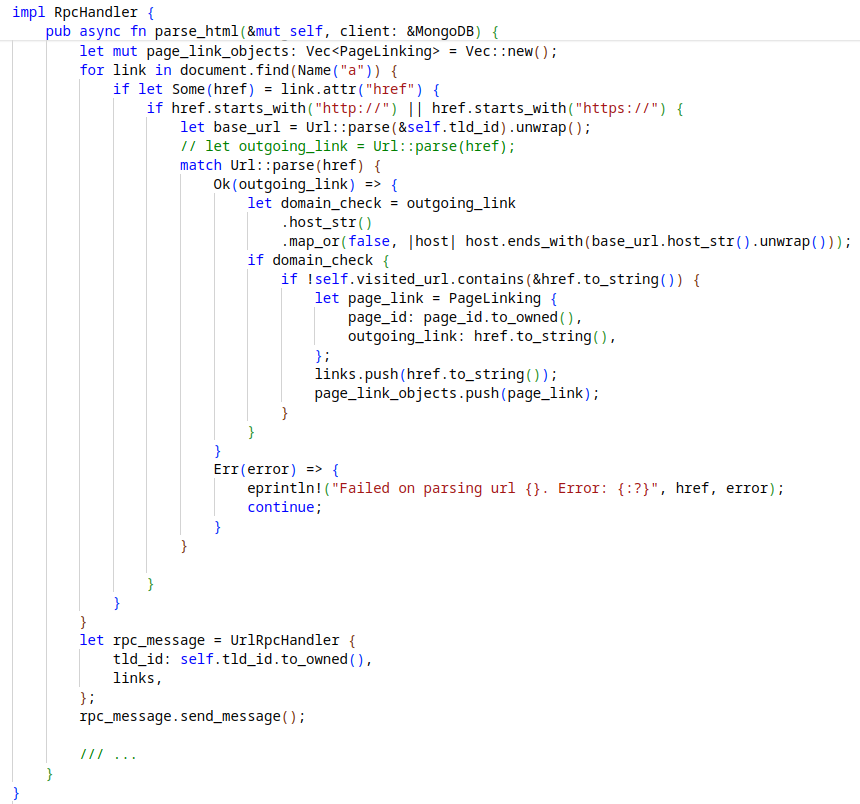
\includegraphics[keepaspectratio, width=12cm]{gambar/parse-link-gathering.png}
  \caption{Bagian kode \emph{parsing} yang melakukan \emph{filtering} terhadap url yang dikumpulkan}
  \label{gambar:parse-link-filtering}
\end{figure}

Mekanisme pembagian tiap domain pada gambar \ref{gambar:thread-manager-start-bfs} hanya dilakukan sekali saja saat \emph{startup}. Ketika \emph{scouter} sedang berjalan dan menerima \emph{incoming url} dari \emph{parser}, \emph{scouter} melakukan pengecekan terhadap pesan masuk tersebut untuk menentukan \emph{list of url} yang masuk berasal dari halaman web dengan \emph{domain} apa. \emph{List or url} tersebut di tambahkan kedalam \emph{queue} yang \emph{domain}-nya sesuai dengan \emph{domain id} dari pesan tersebut.

\begin{figure}[H]
  \centering
  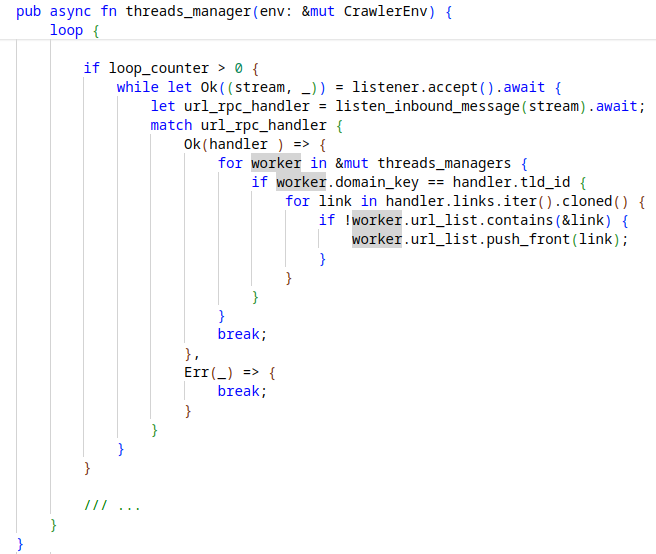
\includegraphics[keepaspectratio, width=12cm]{gambar/scouter-listen-links.png}
  \caption{Bagian kode untuk membagi url kedalam masing-masing \emph{thread}}
  \label{gambar:scouter-listen-bfs}
\end{figure}

\subsection{\emph{Scouter Service}}

\begin{figure}[H]
  \centering
  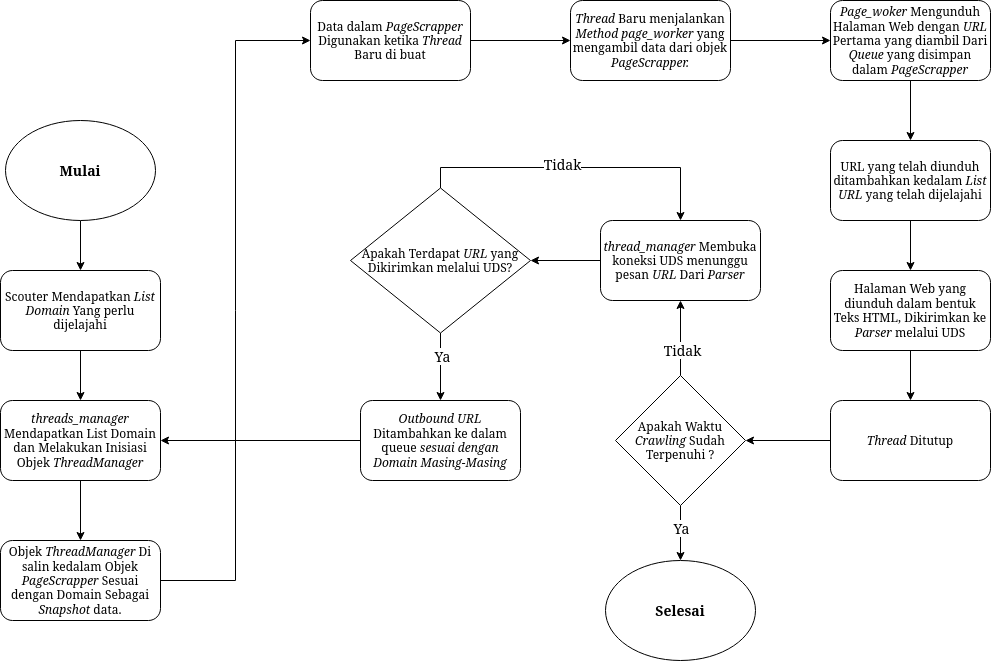
\includegraphics[keepaspectratio, width=10cm]{gambar/scouter-flowchart.png}
  \caption{\emph{Flowchart} dari mekanisme jalannya \emph{scouter service}}
  \label{gambar:scouter-flowchart}
\end{figure}

\emph{Scouter} sebagai \emph{services} yang bertugas sebagai \emph{entry point}, manajemen akses \emph{crawler} dalam menjelajahi halaman web, kontrol terhadap algoritma \emph{breadth-first search} termodifikasi, \emph{thread manager}, dan pengunduh halaman web kedalam bentuk teks \emph{HTML}. \emph{Scouter} secara umum bertugas mendapatkan daftar \emph{origin url} yang perlu dijelajahi, memasukkannya kedalam \emph{queue} per \emph{top-level domain}, mengakses \emph{url-url} tersebut menggunakan \emph{HTTP Call}, mengirimkan halaman web yang telah diunduh melalui \emph{Unix Domain Socket}, dan membuka koneksi \emph{UDS} dari \emph{parser} yang berisi daftar \emph{outbound url} yang dikumpulkan oleh \emph{parser} dari satu halaman.

\begin{figure}[H]
  \centering
  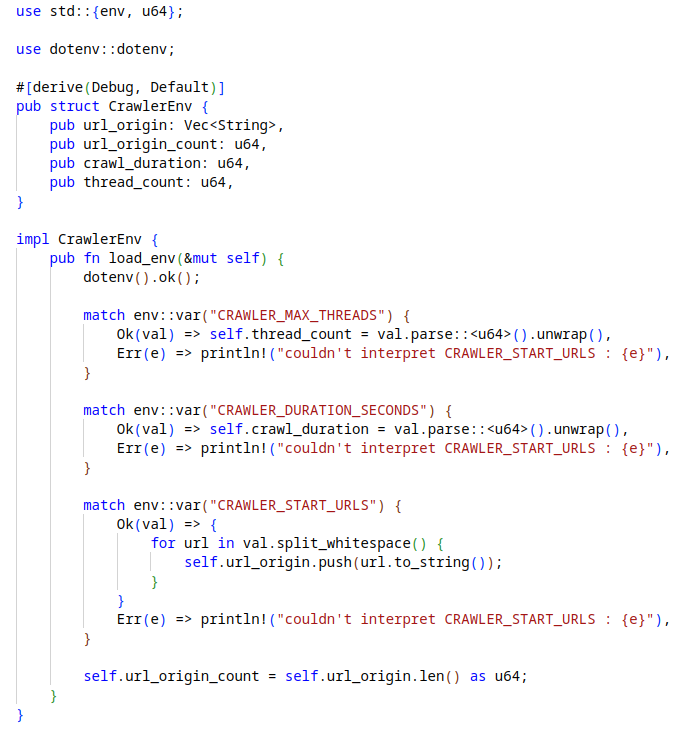
\includegraphics[keepaspectratio, width=13cm]{gambar/get_env_code.png}
  \caption{Fungsi \emph{load\_env} dalam \emph{scouter service} yang berfungsi untuk mendapatkan daftar \emph{url} dari \emph{environment variable}}
  \label{gambar:get_env_code}
\end{figure}

Diagram \ref{gambar:scouter-flowchart} menggambarkan alur keseluruhan dari \emph{scouter}. Daftar domain yang perlu dijelajahi didapatkan dari \emph{environment variables} yang disimpan dalam file \emph{.env}, variable yang disimpan adalah \emph{CRAWLER\_MAX\_THREADS}, \emph{CRAWLER\_DURATION\_SECONDS}, dan \emph{CRAWLER\_START\_URLS}. Gambar \ref{gambar:get_env_code} merupakan mekanisme dari \emph{scouter} dalam mendapatkan daftar \emph{environment variables} kedalam kode. Semua variable tesebut disimpan kedalam \emph{struct} bernama \emph{CrawlerEnv}. Untuk menjalankan mekanisme ini \emph{scouter} hanya perlu membuat objek dengan tipe data \emph{CrawlerEnv} dan memanggil fungsi \emph{load\_env} untuk mengisi objek tersebut dengan \emph{environment variables}. Gambar \ref{gambar:load_env-called} merupakan contoh kode saat fungsi \emph{load\_env()} dipanggil dan mengisi objek \emph{env} yang berisi \emph{environment variables}.

\begin{figure}[H]
  \centering
  \includegraphics[keepaspectratio, width=10cm]{gambar/load_env_called.png}
  \caption{Pemanggilan fungsi \emph{load\_env} dalam fungsi \emph{main()}}
  \label{gambar:load_env-called}
\end{figure}

Kode dalam gambar \ref{gambar:load_env-called} juga menunjukkan objek \emph{env} dipindahkan sebagai paramter dari fungsi \emph{threads\_manager}. Fungsi \emph{threads\_manager} merupakan fungsi utama yang menjalankan fungsionalitas \emph{scouter}.

\begin{figure}[H]
  \centering
  \includegraphics[keepaspectratio, width=10cm]{gambar/code-thread-manager-init.png}
  \caption{Bagian dari fungsi \emph{thread\_manager} yang berfungsi sebagai inisiasi mekanisme \emph{multi-threading}}
  \label{gambar:thread-manager-func-init}
\end{figure}

Gambar \ref{gambar:thread-manager-func-init} merupakan bagian kode dari fungsi \emph{thread\_manager()} dan definisi \emph{struct} \emph{ThreadManager}. Fungsi \emph{thread\_manager()} merupakan fungsi yang mengatur \emph{resource allocation}, menunggu \emph{inbound message} dari \emph{parser}, dan mekanisme pembuatan \emph{thread} baru. Dalam gambar \ref{gambar:thread-manager-func-init} fungsi \emph{thread\_manager()} terlihat melakukan inisiasi \emph{start\_time} yang digunakan untuk mencatat waktu dimulainya proses dan beberapa variable lain yang digunakan untuk \emph{resource allocation} per operasi pengunduhan halaman web. Kode ini juga membuat variable baru yang bernama \emph{thread\_managers}, variable ini berfungsi untuk menampung satu atau lebih objek dengan tipe data \emph{ThreadManager} yang akan digunakan untuk menampung informasi-informasi yang akan digunakan dalam \emph{scope} dari masing-masing \emph{thread}.

\begin{figure}[H]
  \centering
  \includegraphics[keepaspectratio, width=10cm]{gambar/thread_manager-code-loop.png}
  \caption{Bagian kode yang bertugas untuk inisiasi \emph{infinite loop} dan mendeteksi \emph{incoming message} dari \emph{parser service}}
  \label{gambar:code-loop-thread-manager}
\end{figure}

Fungsi \emph{thread\_manager()} juga menjalankan peran sebagai pengatur mekanisme algoritma \emph{breadth-first search} yang digunakan oleh \emph{scouter}, dikarenakan \emph{scouter} ini harus berjalan terus menerus hingga waktu habis maka fungsi \emph{thread\_manager()} harus menjalankan \emph{infinite loop} yang berhenti hanya jika waktu jalannya \emph{scouter} telah terpenuhi. Selain mekanisme \emph{spawn thread}, dalam gambar \ref{gambar:code-loop-thread-manager} juga terdapat kode untuk mendengar \emph{inbound message} dengan melakukan bind dengan \emph{socket file} \emph{/tmp/temp-onecrawl-url.sock}. Fungsi \emph{listen\_inbound\_message()} merupakan fungsi untuk menerima \emph{inbound message} tersebut dan mengembalikan objek yang berisi \emph{message} yang telah di \emph{parse}.

\begin{figure}[H]
  \centering
  \includegraphics[keepaspectratio, width=10cm]{gambar/thread_manager_spawn_code.png}
  \caption{Bagian kode dari fungsi \emph{thread\_manager} yang berfungsi untuk \emph{spawning thread} tiap \emph{url} masuk}
  \label{gambar:thread-manager-spawn-code}
\end{figure}

Dalam setiap iterasi \emph{loop}, \emph{scouter} menjalankan proses pengunduhan dalam \emph{thread} yang terisolasi. Untuk menghindari komplikasi waktu dari proses \emph{locking} dan \emph{race condition} saat \emph{dequeue} setiap thread memiliki \emph{queue} masing-masing. Untuk menghentikan semua proses dalam \emph{thread} yang sedang berjalan secara \emph{graceful} menggunakan \emph{atomic variable} bernama \emph{running}, saat \emph{thread} baru dibuat, setiap \emph{thread} berjalan dengan konteks \emph{Ordering::relaxed} dan proses dalam \emph{threads} hanya akan berjalan jika \emph{Ordering::relaxed} bernilai benar atau \emph{true}. Dengan mekanisme ini kode dapat di kustomisasi sehingga bila sejumlah waktu telah dicapai, variable \emph{running} dapat diubah statusnya dari \emph{Ordering::relaxed} dengan status \emph{true} menjadi \emph{false}, ini akan memicu mekanisme dalam \emph{thread} untuk berhenti.

\begin{figure}[H]
  \centering
  \includegraphics[keepaspectratio, width=10cm]{gambar/page_worker-code.png}
  \caption{ Fungsi \emph{page\_worker} untuk melakukan pengunduhan halaman web}
  \label{gambar:page-worker-code}
\end{figure}

Dari gambar \ref{gambar:thread-manager-spawn-code} dapat dilihat didalam \emph{thread} yang telah dibuat terjadi pemanggilan metode \emph{page\_worker} yang merupakan modul utama pemanggilan \emph{http} dalam \emph{scouter service} , metode ini adalah metode dari objek \emph{page\_woker} yang sudah di buat sebelumnya dan bekerja sebagai fungsi utama yang dieksekusi didalam masing-masing \emph{thread} yang terisolasi. Gambar \ref{gambar:page-worker-code} merupakan potongan kode dari definisi \emph{class} \emph{PageScrapper} yang merupakan \emph{blueprint} dari objek \emph{page\_worker} dan fungsi \emph{page\_worker} itu sendiri. Dari gambar \ref{gambar:page-worker-code} dapat terlihat bahwa fungsi \emph{page\_worker} hanya melakukan dua hal utama yaitu, proses pengunduhan teks \emph{html} dari halaman web dan mengirimkan teks tersebut beserta informasi pendukung lainnya melalui \emph{send\_message}. Objek \emph{raw\_page\_mes} dibuat berdasarkan \emph{class} \emph{RpcMessage}. Fungsi \emph{page\_worker} ini memberikan \emph{return value} \emph{url} yang telah dijelajahi dan status apakah fungsi berhasil dijalankan atau tidak. Gambar \ref{gambar:scouter-flowchart} merupakan gambaran secara umum bagaimana fungsi ini berjalan.

\begin{figure}[H]
  \centering
  \includegraphics[keepaspectratio, width=10cm]{gambar/scouter-multithread-diagram.png}
  \caption{Diagram mekanisme \emph{multi-thread} dari \emph{scouter service}}
  \label{gambar:scouter-multithread-diagram}
\end{figure}

\subsection{Komunikasi pengiriman \emph{page} melalui \emph{Unix Domain Socket}} 

Seperti yang ditunjukkan dalam kode di gambar \ref{gambar:page-worker-code} dan diagram dari gambar \ref{gambar:scouter-multithread-diagram} teks \emph{HTML} hasil pengunduhan \emph{scouter}, selanjutnya dikirimkan kepada \emph{parser services} melalui \emph{Unix Domain Socket} atau \emph{UDS}. Proses pengiriman teks ini dilakukan secepatnya setelah proses pengunduhan selesai. Agar parser dapat membaca pesan dengan mudah, struktur \emph{class} dari pesan pada \emph{scouter service} dan \emph{parser service} menggunakan \emph{class} yang sama dan pesan di kirim dalam bentuk \emph{json string}.

\begin{figure}[H]
  \centering
  \includegraphics[keepaspectratio, width=10cm]{gambar/rpc-message-struct.png}
  \caption{Struktur dari pesan \emph{rpc} yang dikirimkan}
  \label{gambar:rpc-struct-scouter}
\end{figure}

Konten pesan yang dikirimkan tidak hanya berisi teks \emph{html} dari halaman yang diunduh tetapi juga \emph{top-level domain} dari halaman tersebut, \emph{visited url} yang telah dijelajahi sampai saat halaman tersebut di unduh, dan \emph{crawl id} dari halaman tersebut.

\begin{figure}[H]
  \centering
  \includegraphics[keepaspectratio, width=13cm]{gambar/rpc-send-message-scouter.png}
  \caption{Fungsi yang mengirim \emph{rpc} message}
  \label{gambar:rpc-send-message-scouter}
\end{figure}

Fungsi \emph{send\_message()} yang terdapat di gambar \ref{gambar:rpc-send-message-scouter} merupakan fungsi untuk mengirim \emph{message} yang di buat sebelumnya melalui koneksi \emph{Unix Domain Socket}. Sebelum pesan dikirimkan pesan tersebut di serialisasi menjadi bentuk \emph{json binary} terlebih dahulu lalu dikirimkan menggunakan metode \emph{write\_all}, melalui jalur \emph{socket} \emph{/tmp/temp-onecrawl-page.sock}. Pesan yang sudah dikirimkan dikirimkan ini nantinya akan diterima oleh \emph{parser service} untuk di proses.


\subsection{\emph{Parser Service}}

\emph{Parser} merupakan \emph{services} yang bertugas sebagai pengekstrak data dan penyimpan data dari halaman-halaman web yang telah diunduh oleh \emph{scouter services}. Halaman web yang sudah berbentuk teks didapatkan oleh \emph{parser} dari \emph{scouter sevices} melalui \emph{uds messages}, data mentah yang didapatkan dari \emph{uds messages} berbentuk \emph{json binary} yang kemudian akan di \emph{deserialize} menjadi suatu \emph{object}. \emph{Object} tersebut yang selanjutnya akan diproses lebih lanjut dan teks \emph{html} yang ada didalam objek tersebut di-\emph{parse} dan diambil data-datanya. Data yang didapat ini yang dimasukkan kedalam \emph{databases}.

\begin{figure}[H]
  \centering
  \includegraphics[keepaspectratio, width=13cm]{gambar/parser-controller-code.png}
  \caption{Bagian kode fungsi \emph{parser\_controller} sebagai \emph{entry point} dari \emph{parser services}}
  \label{gambar:parser-controller}
\end{figure}

Fungsi \emph{parser\_controller()} dari gambar \ref{gambar:parser-controller} merupakan \emph{entry point} dari jalannya seluruh proses dalam \emph{parser service}. Hal pertama yang dilakukan dalam fungsi ini adalah membuka koneksi kedalam \emph{database}, selain itu fungsi ini juga menginisiasi \emph{timestamp} untuk menghitung waktu jalannya \emph{parser} dan inisiasi koneksi \emph{socket}. Proses \emph{binding port} dilakukan di fungsi ini ketika fungsi \emph{bind()} dipanggil, hasil dari funsi itu adalah \emph{listener address} yang dapat digunakan untuk menerima \emph{message} dari \emph{unix domain socket}. Fungsi \emph{listen\_message()} yang dipanggil di dalam \emph{parser\_controller()} merupakan fungsi utama yang menjalankan proses \emph{listening} dari \emph{socket}. Setelah semua mekanisme \emph{parser} selesai \emph{parser\_controller()} akan menghapus dua \emph{file socket} yang telah di buat.

\begin{figure}[H]
  \centering
  \includegraphics[keepaspectratio, width=13cm]{gambar/parser-listen-message.png}
  \caption{Funsgi \emph{listen\_message} sebagai manajemen \emph{timout} mekanisme \emph{listening} untuk pesan masuk dari \emph{scouter}}
  \label{gambar:parser-listen-message}
\end{figure}

Fungsi \emph{listen\_message()} dari gambar \ref{gambar:parser-listen-message} memuat mekanisme \emph{timout} dari parser, singkatnya dikarenakan proses \emph{binding} dari \emph{port} berada di \emph{parser} makan \emph{service} ini perlu dijalankan lebih dahulu dibanding \emph{scouter}. Untuk menghindari inkonsistensi dalam penggunaan \emph{port} yang disebabkan \emph{parser} juga yang menghapus dua file \emph{port} seperti di gambar \ref{gambar:parser-controller} , maka \emph{parser} harus berhenti beberapa detik setelah \emph{scouter} berhenti, ini dapat dicapai dengan menambah batasan waktu selama 30 detik. Selain mekanisme \emph{timeout}, \emph{listen\_message()} juga melakukan \emph{processing} terhadap \emph{binary} dari pesan yang diterima dengan mengubahnya menjadi \emph{string} dan mencari pembatas antar pesan yang berbentuk teks \emph{end crawled message}. Teks pesan yang sudah masuk selanjutnya langsung dipindahkan agar dapat digunakan oleh fungsi \emph{process\_message()} untuk di \emph{deseralized}.

\begin{figure}[H]
  \centering
  \includegraphics[keepaspectratio, width=13cm]{gambar/parser-process-message-code.png}
  \caption{Fungsi \emph{process\_message} sebagai fungsi deserialisasi pesan \emph{socket} kedalam struktur yang jelas}
  \label{gambar:parser-process-message}
\end{figure}

Fungsi \emph{process\_message()} hanya bertugas untuk membersihkan dan melakukan \emph{deserialized} data mentah dari \emph{socket} kedalam objek yang terstruktur, di dalam fungsi ini juga akan dipanggil metode \emph{parse\_html()} fungi ini yang akan melakukan sebagian besar operasi pengambilan data dari halaman web.

\begin{figure}[H]
  \centering
  \includegraphics[keepaspectratio, width=10cm]{gambar/parse-html-body-text.png}
  \caption{Fungsi \emph{parse\_html()} sebagai fungsi utama dalam proses \emph{parsing} halaman web}
  \label{gambar:parse-html-body-text}
\end{figure}

Fungsi \emph{parse\_html()} melakukan penguraian dan pengambilan data dari halaman web yang telah diunduh. Sebelum data diambil untuk memudahkan pengambilan data dilakukan pembuatan \emph{language tree} ketika \emph{class Document} dipanggil, objek \emph{document} yang telah dibuat merupakan \emph{language tree} yang sudah jadi dan dapat dimanimulasi \emph{dom}-nya. Data yang akan diambil dikelompokkan berdasarkan jenis data dan pengaruhnya terhadap jenis informasi yang akan di ambil dari halaman web tersebut. Dalam implementasi \emph{web crawler} ini informasi yang paling penting untuk dikumpulkan adalah teks konten dalam \emph{body html}, data ini dikumpulkan untuk perhitungan \emph{rank} dari tiap-tiap halaman tersebut. Hal ini dapat terlihat di kode dalam gambar \ref{gambar:parse-html-body-text} dimana bagian kode untuk \emph{filtering} dan pengumpulan teks ini di dilakukan pertama kali. Mekanisme pengumpulan ini dilakukan oleh fungsi dengan mengumpulkan seluruh teks didalam \emph{body} dan melakukan filtering pada teks.

\begin{figure}[H]
  \centering
  \includegraphics[keepaspectratio, width=10cm]{gambar/parser-tag-visible.png}
  \caption{Fungsi \emph{tag\_visible()} sebagai fungsi yang melakukan \emph{filtering} pada teks yang dikumpulkan}
  \label{gambar:parse-tag-visible}
\end{figure}

Proses filtering ini dilakukan oleh fungsi \emph{tag\_visible()} yang direferensikan di gambar \ref{gambar:parse-html-body-text}, fungsi ini melakukan filtering terhadap teks yang dikumpulkan. Tujuan dari proses ini adalah agar teks yang bukan konten dari halaman web tidak akan masuk kedalam \emph{database}. Teks yang disaring oleh fungsi ini dapat dilihat di kode dalam gambar \ref{gambar:parse-tag-visible} yaitu teks yang ada didalam \emph{tag} \emph{style}, \emph{script}, \emph{head}, \emph{title}, \emph{meta}, dan \emph{document}. Selain itu fungsi ini juga menyaring \emph{new line} dan \emph{new tab} yang direpresentasikan oleh karakter \emph{"n"} dan \emph{"t"} dari teks yang akan dimasukkan.

\begin{figure}[H]
  \centering
  \includegraphics[keepaspectratio, width=12cm]{gambar/parse-link-gathering.png}
  \caption{Bagian kode dari fungsi \emph{parse\_html()} yang mengumpulkan \emph{outbound url} dari halaman web}
  \label{gambar:parse-link-gathering}
\end{figure}

Selain konten teks \emph{outbound url} juga perlu dikumpulkan, kumpulan \emph{url} ini perlu di saring terlebih dahulu untuk dicek apakah \emph{url} ini merujuk pada \emph{website} dengan domain yang sama atau tidak. Bila \emph{url} merujuk pada domain yang sama, maka akan dikumpulkan. Kumpulan \emph{url} ini selanjutnya akan di masukkan kedalam \emph{database} dan juga dikirimkan ke \emph{scouter service} melaui koneksi \emph{Unix Domain Socket}. \emph{Parser} juga menyimpah informasi-informasi lain seperti \emph{form}, \emph{list}, dan \emph{script} dari halaman web tersebut.

\subsection{Komunikasi balik pengiriman \emph{URL} melalui \emph{Unix Domain Socket}}

\begin{figure}[H]
  \centering
  \includegraphics[keepaspectratio, width=14cm]{gambar/parser-udp-send-message.png}
  \caption{Fungsi \emph{method} dan struktur dari \emph{rpc message} yang dikirimkan oleh \emph{parser service}}
  \label{gambar:parse-send-message}
\end{figure}

Kode pada gambar \ref{gambar:parse-link-gathering} memperlihatkan dipanggilnya fungi \emph{send\_message()}, fungsi ini merupakan mekanisme \emph{parser service} untuk mengirimkan \emph{url} kepada \emph{scouter service}. Kumpulan \emph{url} ini yang akan ditambahkan ke \emph{queue} untuk diakses selanjutnya oleh \emph{scouter}. Gambar \ref{gambar:parse-send-message} merupakan definisi objek dan fungsi dari mekanisme pengiriman pesan ini. Secara general ini merupakan mekanisme yang sama dengan proses pengiriman pesan dari \emph{scouter service} dengan perbedaan pada alamat \emph{file socket} yang digunakan.

\begin{figure}[H]
  \centering
  \includegraphics[keepaspectratio, width=14cm]{gambar/scouter-listen-links.png}
  \caption{Bangian kode dalam \emph{scouter service} yang menerima \emph{rpc message} dari \emph{parser service}}
  \label{gambar:scouter-listen-link}
\end{figure}

Pesan yang sudah dikirimkan oleh \emph{parser} diterima oleh \emph{scouter}, mekanisme \emph{scouter} dalam menerima pesan ini adalah dengan mengumpulkan \emph{url} yang didapatkan dari \emph{socket}, mencocokkannya dengan \emph{top level domain} yang ada di dalam \emph{scouter} dan menyimpannya kedalam \emph{queue} yang sesuai dengan \emph{domain} tersebut, seperti yang terlihat di kode dalam gambar \ref{gambar:scouter-listen-link}.

\subsection{Penyimpanan data dari \emph{Parser} dan model data \emph{Databases}}

Data-data yang sudah dikumpulkan oleh parser seperti teks konten, judul, \emph{form}, \emph{list} dan, lainnya seluruhnya di masukkan kedalam database dengan nama \emph{collection} yang sesuai jenis data tersebut. Data seperti teks konten, judul, dan deskripsi halaman web disimpan dalam \emph{collection} yang bernama \emph{page\_information}, sedangkan informasi yang berhubungan dengan \emph{url} disimpan dalam \emph{page\_links collection} dan seterusnya.

\begin{figure}[H]
  \centering
  \includegraphics[keepaspectratio, width=14.5cm]{gambar/crawler-erd.png}
  \caption{\emph{Entity Relations Diagram} untuk database crawler}
  \label{gambar:erd-crawler}
\end{figure}

Dari gambar \ref{gambar:erd-crawler} dapat dilihat bahwa \emph{id} dari \emph{page\_information} digunkana sebagai \emph{foreign key} di dalam \emph{collection}, karena satu halaman web hanya akan memiliki satu \emph{page\_information} maka masuk akal untuk menjadikan \emph{id} tersebut sebagai \emph{key identifier} di dalam \emph{collection} lain. \emph{Primary key} atau id dari \emph{page\_information} didapat langsung setelah proses \emph{insert} dan disimpan dalam variabel \emph{page\_id}. Variabel ini yang selanjutnya akan digunakan terus menerus ketika proses penyimpanan data

\begin{figure}[H]
  \centering
  \includegraphics[keepaspectratio, width=11cm]{gambar/insert-page-info.png}
  \caption{Bagian kode yang berfungsi untuk memasukkan \emph{page\_information} kedalam \emph{database}}
  \label{gambar:insert-page-info}
\end{figure}

Untuk data-data yangh jumlah nya banyak seperti \emph{url}, \emph{script}, \emph{table}, \emph{list}, \emph{image}, \emph{form}, dan \emph{style} metode penyimpanan yang digunakan adalah \emph{insert\_bulk()} seperti dalam kode di gambar \ref{gambar:bulk-insert} agar seluruh data disimpan sekaligus tanpa menggunakan mekanisme \emph{looping}. Ini akan mempercepat proses penyimpanan data terutama pada halaman web yang memiliki jumlah data yang banyak.

\begin{figure}[H]
  \centering
  \includegraphics[keepaspectratio, width=10cm]{gambar/bulk-insert-code.png}
  \caption{Contoh pemanggilan fungsi \emph{bulk\_insert()} untuk memasukkan lebih dari satu data sekaligus}
  \label{gambar:bulk-insert}
\end{figure}

\subsection{\emph{Shared Utility Library}}

\emph{Onecrawl-util} merupakan \emph{shared library} yang di-digunakan oleh \emph{scouter service} dan \emph{parser service}. \emph{Shared Library} ini dibuat untuk memudahkan pemanggilan dan penggunaan \emph{query} terhadap database \emph{mongodb} yang digunakan di kedua \emph{services} tersebut. Fungsi yang didefinisikan dalam \emph{onecrawl util} yang dapat digunakan \emph{service} lain yaitu \emph{insert\_once()}, \emph{insert\_bulk()}, \emph{get\_inserted\_id()}, \emph{check\_value()}, dan \emph{count\_data()}.

\begin{figure}[H]
  \centering
  \includegraphics[keepaspectratio, width=13cm]{gambar/db-coll-func-util.png}
  \caption{Inisiasi objek \emph{database} yang akan digunakan seterusnya untuk operasi \emph{database}}
  \label{gambar:db-coll-definition}
\end{figure}

Untuk memudahkan inisiasi saat fungsi dipanggil oleh kedua \emph{services}, \emph{library} ini memiliki dua fungsi \emph{db} dan \emph{coll} yang dapat disatukan dengan \emph{chain link} pemanggilannya. Kedua fungsi ini digunakan untuk menginisiasi nama \emph{database} dan \emph{collection} serta mengeneralisasikan \emph{struct} untuk \emph{collection} yang akan berinteraksi dengan fungsi.

\begin{figure}[H]
  \centering
  \includegraphics[keepaspectratio, width=12cm]{gambar/insert-util-code.png}
  \caption{Fungsi operasi \emph{insert} dalam \emph{shared utility library}}
  \label{gambar:insert-util-code}
\end{figure}

Fungsi \emph{insert\_once()} dan \emph{insert\_bulk()} pada gambar \ref{gambar:insert-util-code} merupakan dua fungsi yang paling sering dipanggil dalam kedua \emph{services}. Kedua fungsi ini merupakan fungsi yang melakukan operasi \emph{insert} atau memasukkan data kedalam \emph{database}, dimana seperti nama nya fungsi \emph{insert\_once()} untuk memasukkan satu data dan \emph{insert\_bulk()} untuk memasukkan lebih dari satu data, kedua fungsi ini memiliki dua parameter yaitu \emph{collection} untuk nama \emph{collection} untuk menyimpan data tersebut dan \emph{document} atau \emph{documents} yang merupakan satu data atau \emph{array} dari kumpulan data yang akan dimasukkan.

\begin{figure}[H]
  \centering
  \includegraphics[keepaspectratio, width=12cm]{gambar/util-count-data-code.png}
  \caption{Fungsi operasi \emph{count data} dalam \emph{shared utility library}}
  \label{gambar:count-util-code}
\end{figure}

Fungsi \emph{count\_data()} pada gambar \ref{gambar:count-util-code} merupakan fungsi yang digunakan untuk menghintung jumlah data yang dari parameter di dalam \emph{database}. Fungsi ini memiliki 3 parameter, \emph{collection} yang merupakan target \emph{collection} yang akan dihitung datanya, \emph{field} merupakan \emph{field} atau kolom dari data yang akan dihitung, dan \emph{value} adalah value data yang akan dihitung jumlah nya. Fungsi ini mengembalikan nilai yang berbentuk \emph{unsigned integer} yang merupakan jumah data-nya.

\begin{figure}[H]
  \centering
  \includegraphics[keepaspectratio, width=12cm]{gambar/util-check-value-code.png}
  \caption{Fungsi operasi \emph{check value} dalam \emph{shared utility library}}
  \label{gambar:checkval-util-code}
\end{figure}

Fungsi \emph{check\_value()} pada gambar \ref{gambar:checkval-util-code} merupakan fungsi yang digunakan untuk mengecek dalam \emph{collection} apakah data yang di deskripsikan ada atau tidak. Parameter dari fungsi ini ada 3 yaitu \emph{collection}, \emph{field}, dan \emph{value}, fungsi ini akan mengecek apakah data dengan \emph{field} dan \emph{value} yang didefinisikan dalam parameter ada atau tidak dalam \emph{collection}. Fungsi ini akan mengembalikan bentuk data \emph{boolean} yang menunjukkan apakah data ini ada atau tidak. Gambar \ref{gambar:function-call} merupakan gambaran dimana fungsi-fungsi ini dipanggil dan berinteraksi dengan \emph{service} apa.

\begin{figure}[H]
  \centering
  \includegraphics[keepaspectratio, width=13cm]{gambar/function-call-diagram.png}
  \caption{Diagram pemanggilan fungsi dari \emph{shared library onecrawl-util}}
  \label{gambar:function-call}
\end{figure}

Selain fungsi untuk menjalankan \emph{query}, \emph{library} ini juga menyimpan definisi \emph{class} dari \emph{collection} untuk penyimpanan data tersebut. Seluruh definisi ini disimpan dalam \emph{onecrawl-util} untuk meminimalisir kompleksitas dan mempermudah akses terhadap \emph{class} dari semua \emph{services}. Objek dari \emph{class - class} ini yang nantinya akan digunakan sebagai definisi data yang akan disimpan kedalam database. Kode dalam gambar \ref{gambar:struct-page-info} merupakan definisi \emph{class} dari \emph{collection page\_information} dalam \emph{database}. 

\begin{figure}[H]
  \centering
  \includegraphics[keepaspectratio, width=10cm]{gambar/struct-page-information.png}
  \caption{Definisi struktur dari objek \emph{PageInformation}}
  \label{gambar:struct-page-info}
\end{figure}

Semua deifinisi \emph{class} ini disimpan dalam file \emph{model.rs} dalam \emph{directory} yang memiliki nama yang sesuai dengan nama \emph{collectionnya}, dan semua \emph{class} ini di abstraksikan sehingga dapat diakses dari file \emph{monggodb.rs}.

\begin{figure}[H]
  \centering
  \includegraphics[keepaspectratio, width=4cm]{gambar/file-structure-db-util.png}
  \caption{Struktur \emph{file} dan \emph{folder} dari \emph{database model}}
  \label{gambar:file-structure-db-util}
\end{figure}

\subsection{Pencarian \emph{multi-column}}

\begin{figure}[H]
  \centering
  \includegraphics[keepaspectratio, width=14cm]{gambar/onequery-code.png}
  \caption{Fungsi untuk melakukan \emph{multi-column} search}
  \label{gambar:onequery-code}
\end{figure}

\section{Pengujian \emph{Web Crawler} }

Proses pengujian \emph{web crawler} akan difokuskan pada 3 sisi yaitu jumlah halaman web terkumpul, persebaran \emph{domain} web, dan \emph{resource} terpakai saat \emph{crawler} berjalan terutama \emph{cpu usage} dan \emph{memory usage}.

\subsection{Pengujian Jumlah Halaman Web Tersimpan}

Pada penelitian ini pengujian dilakukan pada 3 \emph{origin url} yaitu "https://detik.com", "https://kompas.com", dan "https://bola.com". Pengujian dilakukan selama 2 jam atau 7200 detik dan menggunakan maksimum 5 \emph{threads}. 

\begin{table}[H]
  \caption{Perbandingan jumlah \emph{row} dari halaman web yang terunnduh}
  \begin{center}
    \begin{tabular}{ |p{5cm}|p{3cm}| } \hline
      \textbf{Jenis \emph{crawler}}& \textbf{Total rows} \\ \hline
      \emph{Old Crawler}&  2900 \\ \hline
      \emph{New Crawler}& 50818 \\ \hline
    \end{tabular}
  \end{center}
\end{table}

Dari jumlah total hasil halaman yang berhasil tersimpan terdapat kenaikan sebesar 17x atau 1700 persen kenaikan jumlah halaman terkumpul.

\subsection{Pengujian Persebaran \emph{Domain} dari halaman web tersimpan}

Aspek lain yang diuji dari \emph{crawler} adalah persebaran antara domain yang berhasi terkumpul.

\begin{table}[H]
  \caption{Persebaran domain dari keseluruhan halaman web yang terunduh}
  \begin{center}
    \begin{tabular}{ |p{3.5cm}|p{3.5cm}|p{3.5cm}| } \hline
      \textbf{https://detik.com}& \textbf{https://kompas.com}& \textbf{https://bola.net} \\ \hline
      38368& 8839& 3611 \\ \hline
    \end{tabular}
  \end{center}
\end{table}

\subsection{Pengujian \emph{language tree durability}}

Untuk menguji proses pembangunan \emph{language tree} dari \emph{crawler} ini, dilakukan proses \emph{crawling} pada dua halaman web dengan struktur yang berbeda untuk membandingkan informasi yang di dapatkan. Pengujian dilakukan terhadap dua halaman web dari domain berita \emph{detik.com} dan domain blog \emph{kaskus.co.id}.

Dari domain \emph{detik.com} halaman yang diuji adalah \emph{https://www.kompas.com/food/read/2024/03/24/111100775/6-cara-bikin-telur-dadar-padang-mengembang-tinggi-ala-restoran}. Dari halaman web ini didapatkan informasi \emph{page\_information sebagai berikut},

\begin{figure}[H]
  \centering
  \includegraphics[keepaspectratio, width=14cm]{gambar/detik-bench-pageinfo.png}
  \caption{Konten dari halaman web \emph{detik.com} yang terunduh}
  \label{gambar:detik-bench-pageinfo}
\end{figure}

Teks kontent yang berhasil dikumpulkan dari halaman web ini berjumlah 1650 kata, selain itu dari halaman tersebut juga terkumpul 20 \emph{outbound url}

Untuk domain \emph{kaskus.co.id}, halaman yang diuji adalah \emph{https://www.kaskus.co.id/thread/6609ee1ced160346e4016557/boikot-black-armada-dubes-australia-australia-pendukung-terkuat-republik-indonesia}. Informasi yang dikumpulkan dalam \emph{page\_information} adalah,

\begin{figure}[H]
  \centering
  \includegraphics[keepaspectratio, width=14cm]{gambar/kaskus-bench-pageinfo.png}
  \caption{Konten dari halaman web \emph{kaskus.id} yang terunduh}
  \label{gambar:kaskus-bench-pageinfo}
\end{figure}

Teks konten yang berhasil dikumpulkan berjumlah 82 kata, dengan 19 \emph{outbound url} yang terkumpul.

\subsection{Pengujian Penggunan \emph{CPU Resource}}

Pengukuran penggunaan \emph{cpu resource} menggunakan metode \emph{perf record} dimana pengukuran dilakukan terhadap \emph{core cycyle} atau berapa banyak suatu objek dijalankan oleh \emph{cpu}, ini akan menunjukkan seberapa besar penggunaan \emph{resource} suatu objek relatif terhadap penggunaan \emph{resource} dari keseluruhan \emph{crawler}. Hasil dari pengukuran ditunjukkan dalam bentuk \emph{bar graph}. Berikut merupakan hasil pengukurang \emph{cpu resource} dari kedua \emph{services},

\begin{figure}[H]
  \centering
  \includegraphics[keepaspectratio, width=14cm]{gambar/graph/cpu-bench-parser.png}
  \caption{Pengunaan \emph{cpu resource} \emph{crawler}}
  \label{gambar:cpu-bench-parser}
\end{figure}

Dari diagram dalam gambar \ref{gambar:cpu-bench-parser} dapat di lihat bahwa, penggunaan \emph{cpu resource} terbanyak dilakukan oleh \emph{tokio} sebagai \emph{manager runtime} dari \emph{multi-threading} dan mekanisme \emph{async} yang digunakan oleh kedua \emph{services}.

\subsection{Pengujian Penggunan \emph{Memory Resource}}

Dalam pengujian penggunaan \emph{memory resource} \emph{crawler}, penggunaan \emph{memory} dari dua service dipantau selama jalannya proses \emph{crawling}. Terdapat 3 data yang dipantau dalam pengujian yaitu, 

\begin{enumerate}
  \item{\emph{Memory Allocated}. Total alokasi \emph{memory}}
  \item{\emph{Memory Allocated (never  deallocated)}. Alokasi \emph{memory} yang tidak pernah di dealokasi}
  \item{\emph{Total Usage}. Jumlah total penggunaan \emph{Memory}}
\end{enumerate}

Berikut merupakan hasil \emph{graph} penggunaan \emph{memory} dari \emph{scouter service},

\begin{figure}[H]
  \centering
  \includegraphics[keepaspectratio, width=15cm]{gambar/graph/scouter-total-alloc.png}
  \caption{Total alokasi \emph{memory}}
  \label{gambar:scouter-total-alloc}
\end{figure}

Graph dari gambar \ref{gambar:scouter-total-alloc} Menunjukkan alokasi \emph{memory} mentah dihitung per iterasi waktu, dari graph tersebut dapat dilihat alokasi memory tertinggi dari jalannya program \emph{scouter service} adalah 350 Mb.

\begin{figure}[H]
  \centering
  \includegraphics[keepaspectratio, width=15cm]{gambar/graph/scouter-never-dealloc.png}
  \caption{\emph{memory} yang tidak di dealokasi}
  \label{gambar:scouter-never-dealloc}
\end{figure}

Sedangkan gambar \ref{gambar:parser-never-dealloc} menunjukkan jumlah memori teralokasi yang tidak di bebaskan oleh program, graph ini menunjukkan jumlah \emph{memory} yang bocor atau \emph{memory leak} dari program. Dari graph dapat diidentifikasi terdapat \emph{memory leak} dengan jumlah maksimal 1 Mb.

\begin{figure}[H]
  \centering
  \includegraphics[keepaspectratio, width=15cm]{gambar/graph/scouter-total-usage.png}
  \caption{Total penggunaan \emph{memory}}
  \label{gambar:scouter-total-usage}
\end{figure}

Sedangkan graph \ref{gambar:scouter-total-alloc} menunjukkan total penggunaan memory yang di alokasi dikurang memory yang berhasil dibebaskan, dari graph tersebut dapat di ungkap bahwa total penggunaan memory paling tinggi dari \emph{scouter} adalah sejumlah 700 Mb.

Berikut merupakan hasil \emph{graph} penggunaan \emph{memory} dari \emph{parser service},

\begin{figure}[H]
  \centering
  \includegraphics[keepaspectratio, width=15cm]{gambar/graph/parser-total-alloc.png}
  \caption{Total alokasi \emph{memory}}
  \label{gambar:parser-total-alloc}
\end{figure}

\begin{figure}[H]
  \centering
  \includegraphics[keepaspectratio, width=15cm]{gambar/graph/parser-never-dealloc.png}
  \caption{\emph{memory} yang tidak di dealokasi}
  \label{gambar:parser-never-dealloc}
\end{figure}

\begin{figure}[H]
  \centering
  \includegraphics[keepaspectratio, width=15cm]{gambar/graph/parser-total-usage.png}
  \caption{Total penggunaan \emph{memory}}
  \label{gambar:parser-total-usage}
\end{figure}

Ketiga graph dari ketiga gambar diatas menunjukkan bahwa secara rata-rata penggunaan \emph{memory} dari \emph{parser services} lebih rendah dari \emph{scouter}, dengan fluktuasi alokasi yang lebih fluktuatif juga, hal ini dikarenakan \emph{parser} yang tidak memiliki \emph{thread} sebanyak \emph{crawler}.

\subsection{Analisis Hasil}

Berdasarkan data yang telah dikumpulkan, analisis pengujian adalah sebagai berikut,

\begin{enumerate}
  \item Jumlah halaman web yang berhasil dikumpulkan oleh \emph{crawler} dengan waktu dan \emph{origin url} yang sama mencapai 25x dari \emph{crawler} sebelumnya
  \item Persebaran halaman web antar domain masih tidak berimbang dengan domain \emph{detik.com} mengumpulkan 75.5 persen dari keseluruhan halaman web yang terkumpul. 
  \item Algoritma deteksi dan pengambilan informasi dari \emph{language tree} halaman web masih belum optimal untuk mengambil informasi dari halaman web dengan struktur yang berbeda dari halaman web berita online. Terjadi penurunan jumlah teks konten yang terkumpul sebesar 90 persen, hal juga dipengaruhi faktor bentuk blog yang tak memiliki banyak kata-kata tetapi proses ekstraksi data dari halaman web dengan tipe blog belum sempurna.
  \item Penggunaan \emph{memory} \emph{scouter service} selama berjalan secara fluktuatif dengan pengunaan terbesar mencapai 755 Mb dan penggunaan terkecil mencapai 124 Mb. Sedangkan pengunaan \emph{memory} \emph{parser} jauh lebih kecil dengan pengunaan terbesar hanya mencapai 62 Mb.
\end{enumerate}

Hasil dari pengujian dari sisi peforma menunjukkan \emph{crawler} baru mengalami peningkatan yang signifikan dari sisi jumlah halaman web yang berhasil dikumpulkan, tetapi peningkatan ini memiliki hasil yang tidak terduga yaitu besarnya penggunaan \emph{core resource} dan \emph{memory resource} dari sisi \emph{scouter service} dan tidak merata-nya persebaran domain. Tidak akuratnya dari \emph{crawler} diakibatkan algoritma \emph{breadhth-first search} termodifikasi yang digunakan saat ini hanya membatasi \emph{domain} yang dapat di akses tetapi tidak menangani permasalahan pemerataan jumlah antar \emph{domain} yang sudah di-\emph{whitelisted}.

Besar nya penggunaan \emph{resource} disisi \emph{scouter}, berasal dari implementasi \emph{scouter} berasal dari penggunaan \emph{multi-threading} yang berlebihan dan perbaikan kedepannya harus dipertimbangkan selanjutnya.

%!TEX root = ./template-skripsi.tex
%-------------------------------------------------------------------------------
%                            	BAB IV
%               		KESIMPULAN DAN SARAN
%-------------------------------------------------------------------------------

\chapter{KESIMPULAN DAN SARAN}

\section{Kesimpulan}
Berdasarkan hasil implementasi dan pengujian fitur sistem informasi yang telah dirancang, maka diperoleh kesimpulan sebagai berikut:

\begin{enumerate}
  \item \emph{Crawler} berhasil mengumpulkan data dari halaman web yang \emph{domain}-nya telah di definiskan dalam \emph{origin url}.
  \item Dari perbandingan hasil proses \emph{crawling} bahasa pemograman berabstraksi rendah lebih cocok untuk digunakan dalam \emph{high-intensity application} seperti \emph{web crawler} ini.
  \item Migrasi \emph{database} dari berbasis \emph{SQL} menuju berbasis \emph{MonggoDB} berhasil dan data yang tersimpan konsisten.
  \item \emph{Crawler} yang dirancang menggunakan metode \emph{multi-threading} berhasil mengumpulkan jumlah halaman web lebih banyak daripada \emph{crawler} sebelumnya.
  \item Algoritma \emph{breadth-first search} termodifikasi dalam skripsi ini belum cukup untuk meningkatkan akurasi proses \emph{crawling} terhadap halaman web yang didefiniskan oleh \emph{top-level domain}.
  \item Penggunaan \emph{resource} lebih banyak berada di \emph{scouter service} bila dibandingkan dengan \emph{parser service}.
\end{enumerate}

\section{Saran}
Adapun saran untuk penelitian selanjutnya adalah:
\begin{enumerate} 
  \item Melanjutkan penelitian dalam eksplorasi algoritma \emph{crawler} lain untuk meningkatkan akurasi pengumpulan halaman web yang telah didefinisikan oleh \emph{top-level domain}.
  \item Melanjutkan penelitian dalam eksplorasi algoritma \emph{information retrieval} yang mengakomodasi lebih banyak jenis \emph{website}.
  \item Eksplorasi penggunaan \emph{filesystem} sebagai platform untuk menyimpan data hasil \emph{crawling} untuk mengakomodasi struktur halaman web yang berbeda-berbeda.
  \item Eksplorasi implementasi \emph{distributed crawler} dengan menggunakan skema \emph{multi-threading} dengan bahasa pemograman berabstraksi rendah seperti \emph{Rust}, \emph{C/C++}, atau \emph{Zig}.
\end{enumerate}


% Baris ini digunakan untuk membantu dalam melakukan sitasi
% Karena diapit dengan comment, maka baris ini akan diabaikan
% oleh compiler LaTeX.
\begin{comment}
\bibliography{daftar-pustaka}
\end{comment}


%-----------------------------------------------------------------
%Disini akhir masukan Bab
%-----------------------------------------------------------------


%-----------------------------------------------------------------
% Disini awal masukan untuk Daftar Pustaka
% - Daftar pustaka diambil dari file .bib yang ada pada folder ini
%   juga.
% - Untuk memudahkan dalam memanajemen dan menggenerate file .bib
%   gunakan reference manager seperti Mendeley, Zotero, EndNote,
%   dll.
%-----------------------------------------------------------------
\bibliographystyle{apalike}
\bibliography{daftar-pustaka}
\addcontentsline{toc}{chapter}{DAFTAR PUSTAKA}
%-----------------------------------------------------------------
%Disini akhir masukan Daftar Pustaka
%-----------------------------------------------------------------

\pagestyle{empty}
\chapter*{\centering \large DAFTAR RIWAYAT HIDUP}
\thispagestyle{empty}
\onehalfspacing{}

\begin{wrapfigure}{l}{4cm}
	\vspace{-25pt}
	\begin{center}
		\includegraphics[width=0.27\textwidth]{gambar/pasfoto}
	\end{center}
	\vspace{-40pt}
\end{wrapfigure}

\noindent \textbf{MUHAMMAD DAFFA HARYADI PUTRA.} Lahir di Jakarta, 15 April 2001.
Anak Pertama dari pasangan Bapak Dadang Haryadi dan Ibu Nova Susanti.
Saat ini penulis tinggal di Jl. Haji Adih No. 42A RT 007/RW 004, Kelurahan Pangkalan
Jati Baru, Kecamatan Cinere, Kota Depok, Provinsi Jawa Barat.

\vspace{1cm}
\noindent
\begin{tabular}{lcl}
	No. Ponsel	& :&  081297786180 \\
	Email	& :&  daffahr15@protonmail.com
\end{tabular}
\vspace{0.5cm}

\noindent \textbf{Riwayat Pendidikan} : Penulis mengikuti pendidikan sekolah
dasar di SD Islam Plus Al-Hasaniah pada tahun 2007 - 2013. Setelah itu,
penulis melanjutkan pendidikan di SMP Negeri 96 Jakarta pada tahun
2013 - 2016. Kemudian penulis melanjutkan pendidikan di SMA Negeri 1 Depok pada
tahun 2016 - 2019. Setelah lulus SMA penulis menjalani jenjang perkuliahan di 
Universitas Negeri Jakarta pada tahun 2019.

\noindent \textbf{Riwayat Organisasi} : Selama di bangku perkuliahan, penulis 
terlibat dalam organisasi kemahasiswaan DEFAULT periode 2021/2022, di mana penulis membantu dalam upaya 
membangun ulang organisasi tersebut kembali sebagai Ketua Umum.

\pagestyle{empty}
\chapter*{\centering \large METADATA}
\thispagestyle{empty}
\onehalfspacing{}

\vspace{2cm}
\noindent
\begin{tabular}{lcl}
	Judul	& :&  Perancangan Improvisasi Arsitektur Web Crawler\\
	& & Berbasis Multi-Threading dan Multi-Processing\\
	& & Dengan Menggunakan Bahasa Pemograman Rust \\
	Nama	& :&  Muhammad Daffa Haryadi Putra \\
	NIM	& :&  1313619034 \\
	Pembimbing I	& :&  Muhammad Eka Suryana, M.Kom \\
	Pembimbing II	& :&  Med Irzal, M.Kom \\
	Keyword	& :& 1. Mesin Pencari \\
  & & 2. \emph{Crawling} \\
  & & 3. \emph{Web Scraping} \\
  & & 4. \emph{Multi-Thread} \\
  & & 5. \emph{Multi-Processes} \\
	& & 6. Teori Informasi
\end{tabular}
\vspace{0.5cm}


\end{document}
